\documentclass[UTF8,11pt]{ctexart}
\usepackage[a4paper,margin=19mm]{geometry}
\usepackage{amsmath,amssymb,tikz,graphicx,hyperref}
\usetikzlibrary{arrows.meta,decorations.pathmorphing}
\setlength{\parindent}{0pt}\setlength{\parskip}{6pt}
\sloppy\emergencystretch=3em

% Site layout only: preserve text, mathematics and native chemical diagrams.
\setlength{\parskip}{2pt}
\raggedbottom
\let\originalenumerate\enumerate
\renewcommand{\enumerate}{\originalenumerate
 \setlength{\itemsep}{2pt}\setlength{\parsep}{0pt}\setlength{\topsep}{3pt}}
\makeatletter
\renewcommand\subsection{\@startsection{subsection}{2}{\z@}
 {-1.1ex\@plus -.3ex\@minus -.2ex}{.5ex\@plus .2ex}
 {\normalfont\normalsize\bfseries}}
\makeatother

\begin{document}\newsavebox{\mockquestionbox}
\begin{center}{\LARGE 南京工业大学637有机化学}\par\medskip{\Large D20 综合平均型模拟卷 详细解析}\par\medskip 满分150分\quad 考试时间180分钟\end{center}本解析供交卷后核对。采分点为训练建议，不是学校官方评分。等效、化学成立且满足题限的解法应酌情给分。\par\section*{一、填空、命名与完成反应（15题，共30分）}\subsection*{1．（2分）}写出下列化合物的中英文名称。\begin{center}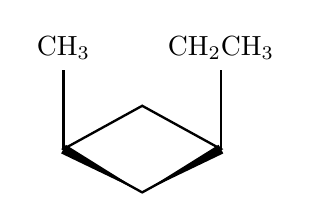
\begin{tikzpicture}[line width=.85pt,>=Stealth]\draw(-1,0)--(0,.55)--(1,0)--(0,-.55)--cycle;\draw(-1,0)--(-1,1)node[above]{$\mathrm{CH_3}$};\draw(1,0)--(1,1)node[above]{$\mathrm{CH_2CH_3}$};\fill(0,-.55)--(-1.03,-.055)--(-.97,.055)--cycle;\fill(0,-.55)--(.97,.055)--(1.03,-.055)--cycle;\end{tikzpicture}\end{center}\subsection*{答案与结构}顺-1-甲基-3-乙基环丁烷（本教材编号）；cis-3-ethyl-1-methylcyclobutane。按英文取代基字母顺序优先编号的cis-1-ethyl-3-methylcyclobutane亦为同一正确结构。\subsection*{从概念到解法}\begin{enumerate}\item 母体是四碳环，两个取代基在相对的1,3位。原透视图两个取代键均朝同一侧，故为cis。\item 中文遵循本教材习惯给甲基1位；英文现代编号遇1,3平局可使字母在前的ethyl取1位。必须保留cis，不能把1,3误读为1,2。\item 这种透视图没有指定一对可分离绝对构型；此连接的两个环路径等价，不应无依据再加R/S。\end{enumerate}\subsection*{验算与易错}环4+Me1+Et2=7个碳。；同面关系由透视方向判断，不是纸面标签都在上方就可对任意图判cis。\subsection*{参考采分（非官方）}连接命名1分；cis及英文完整1分。\par 来源：S01，2-9(ii)，印刷页11，PDF页17。\par\medskip\clearpage\subsection*{2．（2分）}完成下列反应，写出主要产物。\begin{center}\begin{tikzpicture}[line width=.85pt,>=Stealth]\draw (-1.589,-1.448)--(0.027,-0.514);
\draw (-1.644,-1.352)--(-0.027,-0.419);
\draw (0.000,-0.467)--(1.617,-1.400);
\draw (0.000,-0.467)--(0.000,1.400);\draw[->](2.7,0)--(5.5,0)node[midway,above,align=center]{$\mathrm{CHCl_3}$\\$\mathrm{t{-}BuOK/t{-}BuOH}$};\node at(7.8,0){\rule{2.5cm}{.3pt}};\end{tikzpicture}\end{center}\subsection*{答案与结构}1,1-二氯-2,2-二甲基环丙烷。\begin{center}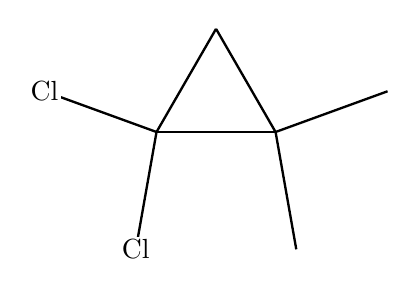
\begin{tikzpicture}[line width=.85pt,>=Stealth]\draw (2.178,0.607)--(0.756,0.090);
\draw (0.756,0.090)--(1.019,-1.400);
\draw (0.756,0.090)--(0.000,1.400);
\draw (0.000,1.400)--(-0.756,0.090);
\draw (-0.756,0.090)--(-1.019,-1.400);
\draw (-0.756,0.090)--(-2.178,0.607);
\draw (-0.756,0.090)--(0.756,0.090);
\node[fill=white,inner sep=1.1pt]at(-1.019,-1.400){$\mathrm{Cl}$};
\node[fill=white,inner sep=1.1pt]at(-2.178,0.607){$\mathrm{Cl}$};\end{tikzpicture}\end{center}\subsection*{从概念到解法}\begin{enumerate}\item 强碱从氯仿夺H后，经\(\alpha\)消除形成二氯卡宾。卡宾碳带两个Cl，是新增的环碳，而不是氯直接对双键逐个加成。\item 卡宾跨双键生成两根新C-C键；原来的两个烯碳加一个卡宾碳成为三元环。原烯一个碳带两个Me，所以产物同一环碳带两个Me。\item 该底物两个Me等同，另一个烯碳是CH2，产物不产生手性中心，不需要写外消旋。\end{enumerate}\subsection*{验算与易错}底物4C加卡宾1C得5C。；两个Cl同在新增碳上，两个Me同在原来较多取代碳上。\subsection*{参考采分（非官方）}三元环及两个Cl1分；两个Me位置1分。\par 来源：S01，8-17(iii)，印刷页136，PDF页142。\par\medskip\clearpage\subsection*{3．（2分）}写出丙二酸二乙酯在乙醇钠乙醇溶液中与下列化合物反应的化学方程式。\begin{center}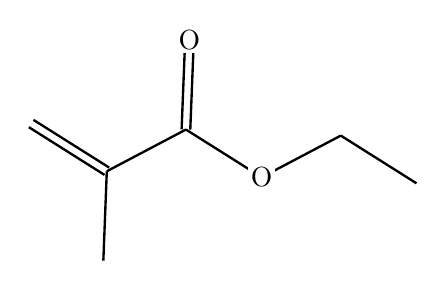
\begin{tikzpicture}[line width=.85pt,>=Stealth]\draw (-2.476,0.295)--(-1.515,-0.311);
\draw (-2.418,0.388)--(-1.456,-0.218);
\draw (-1.486,-0.265)--(-1.530,-1.400);
\draw (-1.486,-0.265)--(-0.481,0.265);
\draw (-0.426,0.263)--(-0.381,1.398);
\draw (-0.536,0.267)--(-0.491,1.402);
\draw (-0.481,0.265)--(0.481,-0.341);
\draw (0.481,-0.341)--(1.486,0.188);
\draw (1.486,0.188)--(2.447,-0.418);
\node[fill=white,inner sep=1.1pt]at(-0.436,1.400){$\mathrm{O}$};
\node[fill=white,inner sep=1.1pt]at(0.481,-0.341){$\mathrm{O}$};\end{tikzpicture}\end{center}\subsection*{答案与结构}丙二酸酯负离子对甲基丙烯酸乙酯作Michael加成，得到$\mathrm{(EtOOC)_2CHCH_2CH(CH_3)COOEt}$。\begin{center}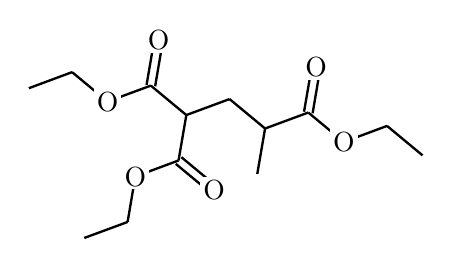
\begin{tikzpicture}[line width=.85pt,>=Stealth]\draw (-2.500,0.646)--(-1.951,0.850);
\draw (-1.951,0.850)--(-1.500,0.476);
\draw (-1.500,0.476)--(-0.951,0.679);
\draw (-0.896,0.670)--(-0.798,1.247);
\draw (-1.005,0.688)--(-0.906,1.266);
\draw (-0.951,0.679)--(-0.500,0.305);
\draw (-0.500,0.305)--(0.049,0.508);
\draw (0.049,0.508)--(0.500,0.134);
\draw (0.500,0.134)--(0.401,-0.443);
\draw (0.500,0.134)--(1.049,0.337);
\draw (1.104,0.328)--(1.202,0.906);
\draw (0.995,0.347)--(1.094,0.924);
\draw (1.049,0.337)--(1.500,-0.037);
\draw (1.500,-0.037)--(2.049,0.167);
\draw (2.049,0.167)--(2.500,-0.207);
\draw (-0.500,0.305)--(-0.599,-0.272);
\draw (-0.634,-0.315)--(-0.183,-0.689);
\draw (-0.563,-0.230)--(-0.113,-0.604);
\draw (-0.599,-0.272)--(-1.148,-0.476);
\draw (-1.148,-0.476)--(-1.246,-1.053);
\draw (-1.246,-1.053)--(-1.796,-1.256);
\node[fill=white,inner sep=1.1pt]at(-1.500,0.476){$\mathrm{O}$};
\node[fill=white,inner sep=1.1pt]at(-0.852,1.256){$\mathrm{O}$};
\node[fill=white,inner sep=1.1pt]at(1.148,0.915){$\mathrm{O}$};
\node[fill=white,inner sep=1.1pt]at(1.500,-0.037){$\mathrm{O}$};
\node[fill=white,inner sep=1.1pt]at(-0.148,-0.646){$\mathrm{O}$};
\node[fill=white,inner sep=1.1pt]at(-1.148,-0.476){$\mathrm{O}$};\end{tikzpicture}\end{center}\subsection*{从概念到解法}\begin{enumerate}\item 丙二酸二乙酯两个羰基之间的CH2去质子化后，负电荷由两羰基稳定，形成碳亲核体。\item 甲基丙烯酸乙酯的C=C与酯羰基共轭，末端CH2为\(\beta\)碳。丙二酸酯中心碳与该\(\beta\)碳成新键；\(\pi\)电子移向羰基形成烯醇盐。\item 乙醇给烯醇盐质子，恢复酯羰基。净产物连接是丙二酸酯中心-CH2-CH(Me)-COOEt，不能把Me位置移到新增CH2。\item 题目没有酸水解、加热脱羧条件，所以保留全部三个乙酯基；不自动套丙二酸合成的脱羧步骤。\end{enumerate}\subsection*{验算与易错}7C丙二酸酯+6C受体=13C产物。；三酯基全部保留；新C-C键连在原\(\beta\)碳。\subsection*{参考采分（非官方）}新C-C连接1分；三个乙酯与Me位置完整1分。\par 来源：S01，10-19(ii)，印刷页189，PDF页195。\par\medskip\clearpage\small \subsection*{4．（2分）}完成下列反应，写出主要产物。\begin{center}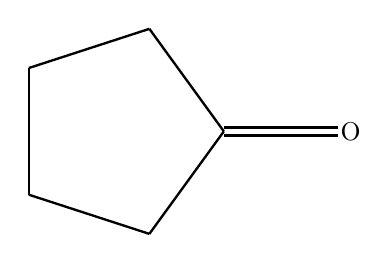
\begin{tikzpicture}[scale=.93,transform shape,line width=.85pt,>=Stealth]\draw (2.197,0.055)--(0.466,0.055);
\draw (2.197,-0.055)--(0.466,-0.055);
\draw (0.466,0.000)--(-0.551,1.400);
\draw (-0.551,1.400)--(-2.197,0.865);
\draw (-2.197,0.865)--(-2.197,-0.865);
\draw (-2.197,-0.865)--(-0.551,-1.400);
\draw (-0.551,-1.400)--(0.466,0.000);
\node[fill=white,inner sep=1.1pt]at(2.197,0.000){$\mathrm{O}$};\end{tikzpicture}\end{center}\[+\ \text{吗啉}\ \xrightarrow{\mathrm{H^+}}\boxed{\phantom{AAAA}}\xrightarrow{\mathrm{ClCH_2COOC_2H_5}}\boxed{\phantom{AAAA}}\xrightarrow{\mathrm{H^+,H_2O}}\boxed{\phantom{AAAA}}\]\begin{center}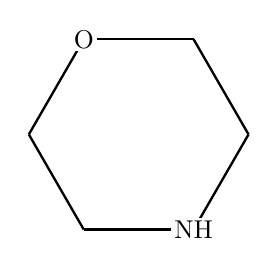
\begin{tikzpicture}[scale=.93,transform shape,line width=.85pt,>=Stealth]\draw (1.500,0.000)--(0.750,1.299);
\draw (0.750,1.299)--(-0.750,1.299);
\draw (-0.750,1.299)--(-1.500,0.000);
\draw (-1.500,0.000)--(-0.750,-1.299);
\draw (-0.750,-1.299)--(0.750,-1.299);
\draw (0.750,-1.299)--(1.500,0.000);
\node[fill=white,inner sep=1.1pt]at(-0.750,1.299){$\mathrm{O}$};
\node[fill=white,inner sep=1.1pt]at(0.750,-1.299){$\mathrm{NH}$};\end{tikzpicture}\end{center}\subsection*{答案与结构}依次为环戊酮的吗啉烯胺、\(\alpha\)位引入CH2COOEt的亚胺正离子氯盐、水解后的2-(乙氧羰基甲基)环戊酮。\begin{center}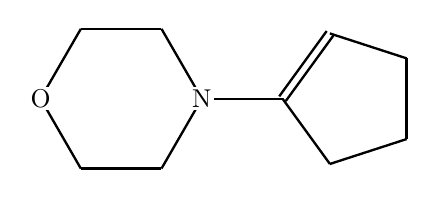
\begin{tikzpicture}[scale=.93,transform shape,line width=.85pt,>=Stealth]\draw (1.408,0.924)--(0.760,0.032);
\draw (1.497,0.859)--(0.849,-0.032);
\draw (0.805,0.000)--(-0.297,0.000);
\draw (-0.297,0.000)--(-0.848,0.954);
\draw (-0.848,0.954)--(-1.949,0.954);
\draw (-1.949,0.954)--(-2.500,0.000);
\draw (-2.500,0.000)--(-1.949,-0.954);
\draw (-1.949,-0.954)--(-0.848,-0.954);
\draw (0.805,0.000)--(1.452,-0.891);
\draw (1.452,-0.891)--(2.500,-0.551);
\draw (2.500,-0.551)--(2.500,0.551);
\draw (2.500,0.551)--(1.452,0.891);
\draw (-0.848,-0.954)--(-0.297,0.000);
\node[fill=white,inner sep=1.1pt]at(-0.297,0.000){$\mathrm{N}$};
\node[fill=white,inner sep=1.1pt]at(-2.500,0.000){$\mathrm{O}$};\end{tikzpicture}\end{center}\begin{center}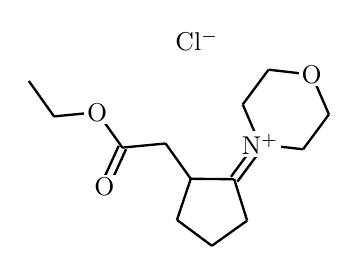
\begin{tikzpicture}[scale=.93,transform shape,line width=.85pt,>=Stealth]\draw (-2.049,0.850)--(-1.705,0.367);
\draw (-1.705,0.367)--(-1.115,0.424);
\draw (-1.115,0.424)--(-0.772,-0.059);
\draw (-0.822,-0.036)--(-1.068,-0.575);
\draw (-0.722,-0.082)--(-0.968,-0.621);
\draw (-0.772,-0.059)--(-0.182,-0.003);
\draw (-0.182,-0.003)--(0.162,-0.485);
\draw (0.162,-0.485)--(-0.026,-1.047);
\draw (-0.026,-1.047)--(0.450,-1.400);
\draw (0.450,-1.400)--(0.932,-1.056);
\draw (0.932,-1.056)--(0.755,-0.491);
\draw (0.799,-0.524)--(1.152,-0.048);
\draw (0.710,-0.458)--(1.063,0.018);
\draw (1.107,-0.015)--(1.696,-0.082);
\draw (1.696,-0.082)--(2.049,0.394);
\draw (2.049,0.394)--(1.813,0.937);
\draw (1.813,0.937)--(1.224,1.005);
\draw (1.224,1.005)--(0.872,0.529);
\draw (0.755,-0.491)--(0.162,-0.485);
\draw (0.872,0.529)--(1.107,-0.015);
\node[fill=white,inner sep=1.1pt]at(0.247,1.400){$\mathrm{Cl^{-}}$};
\node[fill=white,inner sep=1.1pt]at(-1.115,0.424){$\mathrm{O}$};
\node[fill=white,inner sep=1.1pt]at(-1.018,-0.598){$\mathrm{O}$};
\node[fill=white,inner sep=1.1pt]at(1.107,-0.015){$\mathrm{N^{+}}$};
\node[fill=white,inner sep=1.1pt]at(1.813,0.937){$\mathrm{O}$};\end{tikzpicture}\end{center}\begin{center}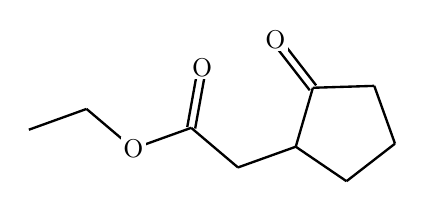
\begin{tikzpicture}[scale=.93,transform shape,line width=.85pt,>=Stealth]\draw (-2.500,-0.266)--(-1.712,0.018);
\draw (-1.712,0.018)--(-1.072,-0.524);
\draw (-1.072,-0.524)--(-0.283,-0.240);
\draw (-0.229,-0.250)--(-0.080,0.575);
\draw (-0.337,-0.230)--(-0.189,0.594);
\draw (-0.283,-0.240)--(0.356,-0.781);
\draw (0.356,-0.781)--(1.145,-0.498);
\draw (1.145,-0.498)--(1.838,-0.969);
\draw (1.838,-0.969)--(2.500,-0.456);
\draw (2.500,-0.456)--(2.217,0.333);
\draw (2.217,0.333)--(1.379,0.307);
\draw (1.423,0.340)--(0.909,1.003);
\draw (1.336,0.273)--(0.822,0.935);
\draw (1.379,0.307)--(1.145,-0.498);
\node[fill=white,inner sep=1.1pt]at(-1.072,-0.524){$\mathrm{O}$};
\node[fill=white,inner sep=1.1pt]at(-0.135,0.584){$\mathrm{O}$};
\node[fill=white,inner sep=1.1pt]at(0.866,0.969){$\mathrm{O}$};\end{tikzpicture}\end{center}\subsection*{从概念到解法}\begin{enumerate}\item 二级胺与酮缩合经脱水、\(\alpha\)去质子形成烯胺；环戊酮两个\(\alpha\)位对称，只有一种烯胺连接。\item 烯胺\(\alpha\)碳为碳亲核位点，进攻氯乙酸乙酯的CH2并置换Cl，形成C-C键和亚胺正离子正离子。Cl负离子作反离子，不能漏电荷把N画成五价中性。\item 酸性水解使C=N回到C=O，释放吗啉；新增CH2COOEt留在环\(\alpha\)位。酯基不是这个步骤自动完全水解的对象，按原书所问烯胺水解产物保留Et酯。\end{enumerate}\subsection*{验算与易错}中间体N正电与Cl负电配对，价态合理。；最终酮5C环+CH2COOEt4C=9C。；新取代碳成为潜在手性中心，原题无手性控制，不指定唯一绝对构型。\subsection*{参考采分（非官方）}烯胺0.5分；带电亚胺正离子0.5分；最终酮1分。\par 来源：S01，13-13(iii)，印刷页259，PDF页265。\par\medskip\clearpage\normalsize \subsection*{5．（2分）}S02-M02-一-Q04\quad 印刷121页 / PDF130页。\par\bigskip
写出下列化合物的系统名称。
\begin{center}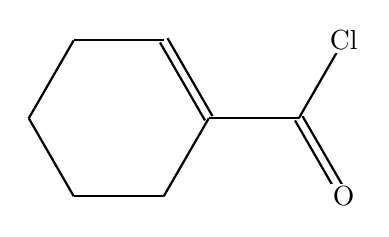
\begin{tikzpicture}[line width=.8pt]\draw (2.048,-0.962)--(1.476,0.028);
\draw (1.952,-1.017)--(1.381,-0.027);
\draw (1.429,0.000)--(2.000,0.990);
\draw (1.429,0.000)--(0.286,0.000);
\draw (0.333,0.028)--(-0.238,1.017);
\draw (0.238,-0.027)--(-0.333,0.962);
\draw (-0.286,0.990)--(-1.429,0.990);
\draw (-1.429,0.990)--(-2.000,0.000);
\draw (-2.000,0.000)--(-1.429,-0.990);
\draw (-1.429,-0.990)--(-0.286,-0.990);
\draw (-0.286,-0.990)--(0.286,0.000);
\node[fill=white,inner sep=1.1pt]at(2.000,-0.990){$\mathrm{O}$};
\node[fill=white,inner sep=1.1pt]at(2.000,0.990){$\mathrm{Cl}$};\end{tikzpicture}\end{center}
\par\medskip\textbf{答案：}环己-1-烯-1-甲酰氯（亦可写1-氯甲酰基环己烯）。
\textbf{推导与理由：}\begin{enumerate}\item 先识别C(=O)Cl为酰氯，不是环上的普通氯代烃。酰氯碳在环外；将带氯甲酰基的环碳编为1，双键在1、2之间。\end{enumerate}
\textbf{反向验算与边界：}\begin{itemize}\item 环为六元；酰氯碳不纳入环；双键相邻羰基连接点。原书答案印刷125页写1-氯甲酰基环己烯。\end{itemize}
 原书答案对照：印刷125页。\par\medskip\clearpage\subsection*{6．（2分）}S02-M02-一-Q07\quad 印刷121页 / PDF130页。\par\bigskip
写出氯化三甲基十二烷基铵的构造式。
\par\medskip\textbf{答案：}$\mathrm{[CH_3(CH_2)_{11}N(CH_3)_3]^+Cl^-}$。
\begin{center}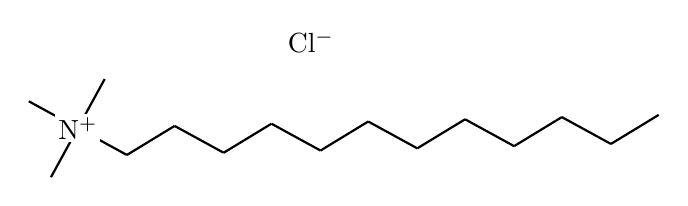
\begin{tikzpicture}[line width=.8pt]\draw (4.000,-0.069)--(3.393,-0.438);
\draw (3.393,-0.438)--(2.770,-0.097);
\draw (2.770,-0.097)--(2.164,-0.466);
\draw (2.164,-0.466)--(1.541,-0.125);
\draw (1.541,-0.125)--(0.934,-0.494);
\draw (0.934,-0.494)--(0.311,-0.153);
\draw (0.311,-0.153)--(-0.295,-0.522);
\draw (-0.295,-0.522)--(-0.918,-0.181);
\draw (-0.918,-0.181)--(-1.525,-0.550);
\draw (-1.525,-0.550)--(-2.148,-0.209);
\draw (-2.148,-0.209)--(-2.754,-0.578);
\draw (-2.754,-0.578)--(-3.377,-0.237);
\draw (-3.377,-0.237)--(-3.718,-0.860);
\draw (-3.377,-0.237)--(-3.036,0.386);
\draw (-3.377,-0.237)--(-4.000,0.104);
\node[fill=white,inner sep=1.1pt]at(-3.377,-0.237){$\mathrm{N^{+}}$};
\node[fill=white,inner sep=1.1pt]at(-0.416,0.860){$\mathrm{Cl^{-}}$};\end{tikzpicture}\end{center}
\textbf{推导与理由：}\begin{enumerate}\item 十二烷基是连氮的一条12碳链，另有三个连氮甲基；氮四个碳单键，带一个正电。氯离子是反离子，不与氮画共价键。\end{enumerate}
\textbf{反向验算与边界：}\begin{itemize}\item 长链1个CH3+11个CH2=12碳，另3个甲基总15碳；总电荷0；不是中性叔胺。\end{itemize}
 原书答案对照：印刷125页。\par\medskip\clearpage\subsection*{7．（2分）}S02-M02-一-Q08\quad 印刷121页 / PDF130页。\par\bigskip
写出2-甲基-2-硝基丙烷的构造式。
\par\medskip\textbf{答案：}$\mathrm{(CH_3)_3CNO_2}$。
\begin{center}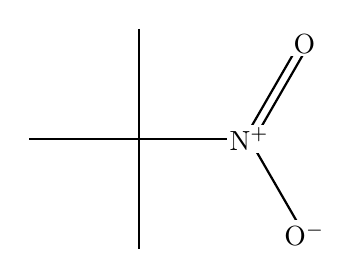
\begin{tikzpicture}[line width=.8pt]\draw (-0.350,1.400)--(-0.350,0.000);
\draw (-0.350,0.000)--(-0.350,-1.400);
\draw (-0.350,0.000)--(-1.750,-0.000);
\draw (-0.350,0.000)--(1.050,0.000);
\draw (1.098,-0.027)--(1.798,1.185);
\draw (1.002,0.028)--(1.702,1.240);
\draw (1.050,0.000)--(1.750,-1.212);
\node[fill=white,inner sep=1.1pt]at(1.050,0.000){$\mathrm{N^{+}}$};
\node[fill=white,inner sep=1.1pt]at(1.750,1.212){$\mathrm{O}$};
\node[fill=white,inner sep=1.1pt]at(1.750,-1.212){$\mathrm{O^{-}}$};\end{tikzpicture}\end{center}
\textbf{推导与理由：}\begin{enumerate}\item 丙烷主链C2连接一个额外甲基和硝基，故中心碳连三个甲基及硝基氮。硝基规范Lewis表达为N正电、一个O负电的共振形式。\end{enumerate}
\textbf{反向验算与边界：}\begin{itemize}\item 中心碳四键；不是亚硝酸叔丁酯，即不画C–O–N；总电荷0。\end{itemize}
 原书答案对照：印刷125页。\par\medskip\clearpage\subsection*{8．（2分）}S02-M02-一-Q03\quad 印刷121页 / PDF130页。\par\bigskip
写出$\mathrm{(CH_3)_3CCHO}$的系统名称。
\par\medskip\textbf{答案：}2,2-二甲基丙醛。
\begin{center}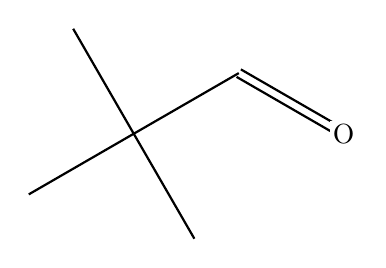
\begin{tikzpicture}[line width=.8pt]\draw (-1.436,1.333)--(-0.667,-0.000);
\draw (-0.667,-0.000)--(0.103,-1.333);
\draw (-0.667,-0.000)--(-2.000,-0.770);
\draw (-0.667,-0.000)--(0.667,0.770);
\draw (0.639,0.722)--(1.972,-0.048);
\draw (0.694,0.817)--(2.027,0.048);
\node[fill=white,inner sep=1.1pt]at(2.000,-0.000){$\mathrm{O}$};\end{tikzpicture}\end{center}
\textbf{推导与理由：}\begin{enumerate}\item 含醛基的最长链为丙醛：醛碳C1，中间季碳C2，末端甲基C3；另外两个甲基均在C2。\end{enumerate}
\textbf{反向验算与边界：}\begin{itemize}\item 总5碳；不是2-甲基丁醛；醛碳必须纳入主链并编号1。\end{itemize}
 原书答案对照：印刷125页。\par 题源替换留痕：原图产物环外=C H2Br使碳五价；不能猜原命题意图，换未用可靠原题。\par\medskip\clearpage\subsection*{9．（2分）}S02-M03-一-Q05\quad 印刷129页 / PDF138页。\par\bigskip
完成下列反应。
\begin{center}\begin{tabular}{ccc}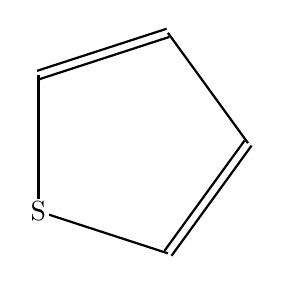
\begin{tikzpicture}[line width=.8pt]\draw (1.331,0.000)--(0.314,1.400);
\draw (0.297,1.452)--(-1.348,0.918);
\draw (0.331,1.348)--(-1.314,0.813);
\draw (-1.331,0.865)--(-1.331,-0.865);
\draw (-1.331,-0.865)--(0.314,-1.400);
\draw (0.359,-1.432)--(1.376,-0.032);
\draw (0.270,-1.368)--(1.287,0.032);
\node[fill=white,inner sep=1.1pt]at(-1.331,-0.865){$\mathrm{S}$};\end{tikzpicture}&$\xrightarrow{\text{浓硫酸，室温}}$&（\qquad）\end{tabular}\end{center}
\par\medskip\textbf{答案：}噻吩-2-磺酸。
\begin{center}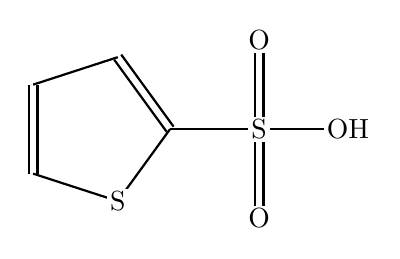
\begin{tikzpicture}[line width=.8pt]\draw (0.925,-1.130)--(0.925,-0.000);
\draw (0.815,-1.130)--(0.815,-0.000);
\draw (0.925,-0.000)--(0.925,1.130);
\draw (0.815,-0.000)--(0.815,1.130);
\draw (0.870,-0.000)--(2.000,-0.000);
\draw (0.870,-0.000)--(-0.261,-0.000);
\draw (-0.216,0.032)--(-0.881,0.947);
\draw (-0.305,-0.032)--(-0.970,0.882);
\draw (-0.925,0.914)--(-2.000,0.565);
\draw (-2.055,0.565)--(-2.055,-0.565);
\draw (-1.945,0.565)--(-1.945,-0.565);
\draw (-2.000,-0.565)--(-0.925,-0.914);
\draw (-0.925,-0.914)--(-0.261,-0.000);
\node[fill=white,inner sep=1.1pt]at(0.870,-1.130){$\mathrm{O}$};
\node[fill=white,inner sep=1.1pt]at(0.870,-0.000){$\mathrm{S}$};
\node[fill=white,inner sep=1.1pt]at(0.870,1.130){$\mathrm{O}$};
\node[fill=white,inner sep=1.1pt]at(2.000,-0.000){$\mathrm{OH}$};
\node[fill=white,inner sep=1.1pt]at(-0.925,-0.914){$\mathrm{S}$};\end{tikzpicture}\end{center}
\textbf{推导与理由：}\begin{enumerate}\item 先识别条件为浓硫酸，不是浓硝酸；芳杂环发生亲电磺化。噻吩2位进攻形成的$\sigma$复合物有较有利的离域稳定，脱去该位质子恢复芳香性，得到2位磺酸。
\item 2位与5位在未取代噻吩中等价，只算一种连接异构体；不可将环硫原子替成氧或把磺酸写成硫酸酯。\end{enumerate}
\textbf{反向验算与边界：}\begin{itemize}\item 新增基团直接为C–S(=O)2OH；不是C–O–SO3H；环硫保留；取代一个环H。\end{itemize}
 原书答案对照：印刷131页。\par\medskip\clearpage\subsection*{10．（2分）}S02-M03-一-Q07\quad 印刷129页 / PDF138页。\par\bigskip
填入实现下列转化的适当试剂。
\begin{center}\begin{tabular}{ccc}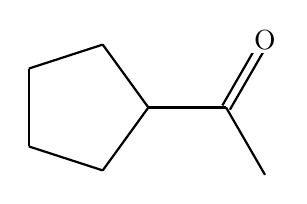
\begin{tikzpicture}[line width=.8pt]\draw (1.500,-0.855)--(1.006,-0.000);
\draw (1.054,-0.028)--(1.548,0.827);
\draw (0.959,0.027)--(1.452,0.882);
\draw (1.006,-0.000)--(0.019,-0.000);
\draw (0.019,-0.000)--(-0.561,0.799);
\draw (-0.561,0.799)--(-1.500,0.494);
\draw (-1.500,0.494)--(-1.500,-0.494);
\draw (-1.500,-0.494)--(-0.561,-0.799);
\draw (-0.561,-0.799)--(0.019,-0.000);
\node[fill=white,inner sep=1.1pt]at(1.500,0.855){$\mathrm{O}$};\end{tikzpicture}&$\xrightarrow{\text{（填试剂）}}$&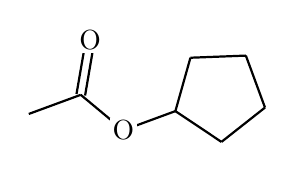
\begin{tikzpicture}[line width=.8pt]\draw (-1.500,-0.291)--(-0.840,-0.048);
\draw (-0.785,-0.057)--(-0.666,0.637);
\draw (-0.894,-0.038)--(-0.774,0.655);
\draw (-0.840,-0.048)--(-0.299,-0.498);
\draw (-0.299,-0.498)--(0.362,-0.255);
\draw (0.362,-0.255)--(0.947,-0.646);
\draw (0.947,-0.646)--(1.500,-0.210);
\draw (1.500,-0.210)--(1.257,0.450);
\draw (1.257,0.450)--(0.553,0.423);
\draw (0.553,0.423)--(0.362,-0.255);
\node[fill=white,inner sep=1.1pt]at(-0.720,0.646){$\mathrm{O}$};
\node[fill=white,inner sep=1.1pt]at(-0.299,-0.498){$\mathrm{O}$};\end{tikzpicture}\end{tabular}\end{center}
\par\medskip\textbf{答案：}过氧酸，例如$\mathrm{CF_3CO_3H}$（原书所列）。
\textbf{推导与理由：}\begin{enumerate}\item 比较结构不是普通醇酯化：酮中环戊基与酰基碳之间插入一个氧，这是Baeyer–Villiger氧化。
\item 过氧酸先加到羰基形成Criegee中间体，环戊基相对甲基有较强迁移倾向；环戊基携成键电子迁移到相邻氧，O–O键断裂，经质子转移得到乙酸环戊酯。\end{enumerate}
\textbf{反向验算与边界：}\begin{itemize}\item 碳数不变、氧数从1到2；产物是环戊基O–COCH3，不是甲基环戊烷甲酸酯；不要求捏造收率。\end{itemize}
 原书答案对照：印刷131页。\par\medskip\clearpage\subsection*{11．（2分）}S02-M05-二-Q01\quad 印刷140页 / PDF149页。\par\bigskip
写出顺-3-甲基环己甲酰胺的最稳定构象。
\par\medskip\textbf{答案：}顺式1,3-二取代双平伏键椅式；两个取代基同面。
\begin{center}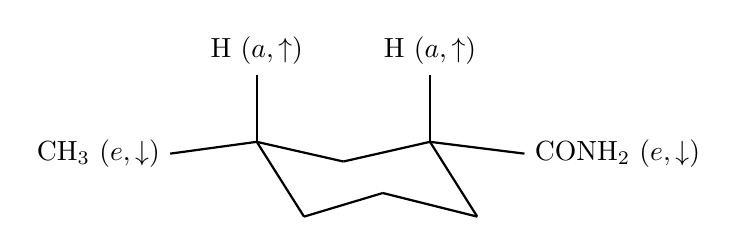
\begin{tikzpicture}[line width=.8pt]\draw(0.800,0.450)--(1.400,-0.500);
\draw(1.400,-0.500)--(0.200,-0.200);
\draw(0.200,-0.200)--(-0.800,-0.500);
\draw(-0.800,-0.500)--(-1.400,0.450);
\draw(-1.400,0.450)--(-0.300,0.200);
\draw(-0.300,0.200)--(0.800,0.450);
\draw(.8,.45)--(2,.3)node[right]{$\mathrm{CONH_2}\ (e,\downarrow)$};
\draw(-1.4,.45)--(-2.5,.3)node[left]{$\mathrm{CH_3}\ (e,\downarrow)$};
\draw(.8,.45)--(.8,1.3)node[above]{$\mathrm H\ (a,\uparrow)$};
\draw(-1.4,.45)--(-1.4,1.3)node[above]{$\mathrm H\ (a,\uparrow)$};\end{tikzpicture}\end{center}
\textbf{推导与理由：}\begin{enumerate}\item 将甲酰胺连接的环碳定为1，甲基在3位，顺式表示两个取代基同面。1、3位的轴向键同面，平伏键也同面，所以可有双轴与双平伏两种翻椅。
\item 双平伏避免两个较大取代基的1,3-二轴排斥，通常更稳定。图中两取代基都向下，整体镜面翻转画成同向上也表达相同相对构型。\end{enumerate}
\textbf{反向验算与边界：}\begin{itemize}\item 酰胺是环–C(=O)NH2，不是环–NH–CHO；不能将顺1,3画成一轴一平伏；翻椅不改变上下。\end{itemize}
 原书答案对照：印刷142页。\par\medskip\clearpage\subsection*{12．（2分）}原书：华东理工大学模拟试题（一） 一、回答问题 第1题；PDF[105]，印刷页[100]。\par\smallskip 命名\par\smallskip \par\smallskip \par\smallskip 用IUPAC命名下列化合物：\par\smallskip 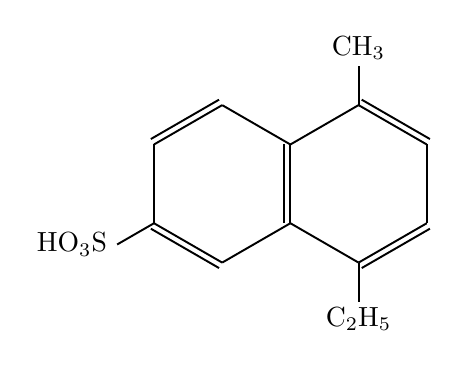
\begin{tikzpicture}[line width=.7pt]\draw(0,0.5)--(0.866,1);
\draw(0.866,1)--(1.732,0.5);
\draw(0.9060008800290411,1.069281524210299)--(1.772000880029041,0.5692815242102991);
\draw(1.732,0.5)--(1.732,-0.5);
\draw(1.732,-0.5)--(0.866,-1);
\draw(1.772000880029041,-0.5692815242102991)--(0.9060008800290411,-1.069281524210299);
\draw(0.866,-1)--(0,-0.5);
\draw(0,-0.5)--(0,0.5);
\draw(-0.08,-0.5)--(-0.08,0.5);
\draw(0,-0.5)--(-0.866,-1);
\draw(-0.866,-1)--(-1.732,-0.5);
\draw(-0.9060008800290411,-1.069281524210299)--(-1.772000880029041,-0.5692815242102991);
\draw(-1.732,-0.5)--(-1.732,0.5);
\draw(-1.732,0.5)--(-0.866,1);
\draw(-1.772000880029041,0.5692815242102991)--(-0.9060008800290411,1.069281524210299);
\draw(-0.866,1)--(0,0.5);
\draw(.866,1)--(.866,1.5);\node at(.866,1.72){$\mathrm{CH_3}$};
\draw(.866,-1)--(.866,-1.5);\node at(.866,-1.72){$\mathrm{C_2H_5}$};
\draw(-1.732,-.5)--(-2.2,-.77);\node[anchor=east]at(-2.2,-.77){$\mathrm{HO_3S}$};\end{tikzpicture}\par\smallskip \par\smallskip \textbf{答案（顺原空次序）：}\par\smallskip \par\smallskip 5-甲基-8-乙基萘-2-磺酸（亦接受8-乙基-5-甲基萘-2-磺酸）\par\smallskip \par\smallskip \textbf{推导：}磺酸作为主官能团，给其最低位次2。再沿保持该位次的萘编号检查同一环上的两个$\alpha$取代位：甲基位于5，乙基位于8。因此可写5-甲基-8-乙基萘-2-磺酸；按英文取代基字母序排列亦可写8-乙基-5-甲基萘-2-磺酸。\par\smallskip \par\smallskip \textbf{反校：}磺酸通过S直接连环，不是硫酸酯；两个烷基不在同一个苯环的相邻位；主官能团位次优先。\par\smallskip \par\smallskip \textbf{2分参考采分：}萘-2-磺酸主骨架1分；5-Me与8-Et位次均对1分。\par\smallskip \par\smallskip 独立推导后对照本书参考答案PDF110页；有原答案缺笔处以原题碳骨架/反应守恒校正，不盲抄。\par\smallskip \par\medskip\clearpage\subsection*{13．（2分）}原书：华东理工大学模拟试题（一） 一、回答问题 第26题；PDF[107]，印刷页[102]。\par\smallskip 完成反应，填写全部原空\par\smallskip \par\smallskip 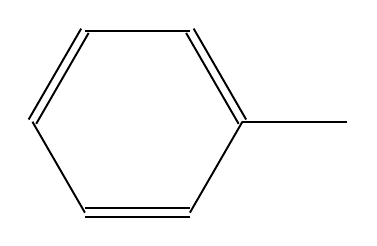
\begin{tikzpicture}[line width=.7pt]\draw (2.000,0.000)--(0.667,0.000);
\draw (0.714,0.028)--(0.048,1.182);
\draw (0.619,-0.027)--(-0.048,1.127);
\draw (0.000,1.155)--(-1.333,1.155);
\draw (-1.381,1.182)--(-2.048,0.028);
\draw (-1.286,1.127)--(-1.952,-0.027);
\draw (-2.000,0.000)--(-1.333,-1.155);
\draw (-1.333,-1.210)--(-0.000,-1.210);
\draw (-1.333,-1.100)--(-0.000,-1.100);
\draw (-0.000,-1.155)--(0.667,0.000);\end{tikzpicture}$\xrightarrow{\ KMnO_4/H^+\ }$（空1）$\xrightarrow{\ NH_3,\Delta\ }$（空2）$\xrightarrow{\ NaOBr,OH^-\ }$（空3）\par\smallskip \par\smallskip \textbf{答案（顺原空次序）：}\par\smallskip \begin{minipage}[c]{.32\linewidth}\centering (1)\par \scalebox{.83}{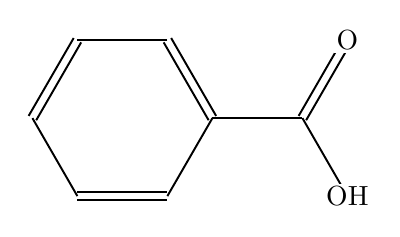
\begin{tikzpicture}[line width=.7pt]\draw (1.952,1.017)--(1.381,0.028);
\draw (2.048,0.962)--(1.476,-0.027);
\draw (1.429,0.000)--(2.000,-0.990);
\draw (1.429,0.000)--(0.286,0.000);
\draw (0.333,0.028)--(-0.238,1.017);
\draw (0.238,-0.027)--(-0.333,0.962);
\draw (-0.286,0.990)--(-1.429,0.990);
\draw (-1.476,1.017)--(-2.048,0.028);
\draw (-1.381,0.962)--(-1.952,-0.027);
\draw (-2.000,0.000)--(-1.429,-0.990);
\draw (-1.429,-1.045)--(-0.286,-1.045);
\draw (-1.429,-0.935)--(-0.286,-0.935);
\draw (-0.286,-0.990)--(0.286,0.000);
\node[fill=white,inner sep=1.1pt]at(2.000,0.990){$\mathrm{O}$};
\node[fill=white,inner sep=1.1pt]at(2.000,-0.990){$\mathrm{OH}$};\end{tikzpicture}}\end{minipage}\begin{minipage}[c]{.32\linewidth}\centering (2)\par \scalebox{.83}{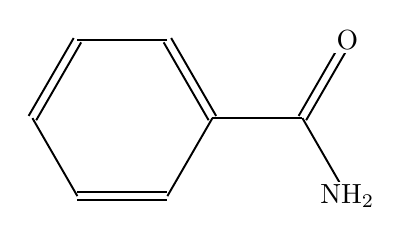
\begin{tikzpicture}[line width=.7pt]\draw (2.000,-0.990)--(1.429,0.000);
\draw (1.476,-0.027)--(2.048,0.962);
\draw (1.381,0.028)--(1.952,1.017);
\draw (1.429,0.000)--(0.286,0.000);
\draw (0.333,0.028)--(-0.238,1.017);
\draw (0.238,-0.027)--(-0.333,0.962);
\draw (-0.286,0.990)--(-1.429,0.990);
\draw (-1.476,1.017)--(-2.048,0.028);
\draw (-1.381,0.962)--(-1.952,-0.027);
\draw (-2.000,0.000)--(-1.429,-0.990);
\draw (-1.429,-1.045)--(-0.286,-1.045);
\draw (-1.429,-0.935)--(-0.286,-0.935);
\draw (-0.286,-0.990)--(0.286,0.000);
\node[fill=white,inner sep=1.1pt]at(2.000,-0.990){$\mathrm{NH_{2}}$};
\node[fill=white,inner sep=1.1pt]at(2.000,0.990){$\mathrm{O}$};\end{tikzpicture}}\end{minipage}\begin{minipage}[c]{.32\linewidth}\centering (3)\par \scalebox{.83}{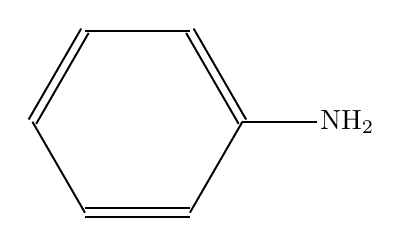
\begin{tikzpicture}[line width=.7pt]\draw (2.000,0.000)--(0.667,0.000);
\draw (0.714,0.028)--(0.048,1.182);
\draw (0.619,-0.027)--(-0.048,1.127);
\draw (0.000,1.155)--(-1.333,1.155);
\draw (-1.381,1.182)--(-2.048,0.028);
\draw (-1.286,1.127)--(-1.952,-0.027);
\draw (-2.000,0.000)--(-1.333,-1.155);
\draw (-1.333,-1.210)--(-0.000,-1.210);
\draw (-1.333,-1.100)--(-0.000,-1.100);
\draw (-0.000,-1.155)--(0.667,0.000);
\node[fill=white,inner sep=1.1pt]at(2.000,0.000){$\mathrm{NH_{2}}$};\end{tikzpicture}}\end{minipage}\par\medskip\par\medskip\par\smallskip \textbf{推导：}苄位甲基有苄氢，被强氧化剂氧化成羧酸。羧酸与氨先成铵盐，再按原印加热条件脱水为伯酰胺。次溴酸盐使伯酰胺发生Hofmann重排，芳基迁移至氮，异氰酸酯水解放出CO2，成为苯胺。\par\smallskip \par\smallskip \textbf{反校：}三空分别C7酸、C7酰胺、C6胺；少一个碳的是酰胺羰基，不是芳环；不能写苄胺。\par\smallskip \par\smallskip \textbf{2分参考采分：}苯甲酸0.5分；苯甲酰胺0.5分；苯胺1分。\par\smallskip \par\smallskip 独立推导后对照本书参考答案PDF111页；有原答案缺笔处以原题碳骨架/反应守恒校正，不盲抄。\par\smallskip \par\medskip\clearpage\subsection*{14．（2分）}原书：华东理工大学模拟试题（一） 一、回答问题 第28题；PDF[107]，印刷页[102]。\par\smallskip 完成反应，填写全部原空\par\smallskip \par\smallskip 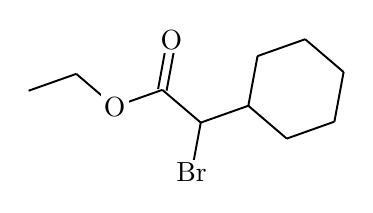
\begin{tikzpicture}[line width=.7pt]\draw (-2.000,0.191)--(-1.395,0.405);
\draw (-1.395,0.405)--(-0.907,-0.012);
\draw (-0.907,-0.012)--(-0.302,0.202);
\draw (-0.248,0.192)--(-0.131,0.823);
\draw (-0.356,0.212)--(-0.240,0.843);
\draw (-0.302,0.202)--(0.186,-0.214);
\draw (0.186,-0.214)--(0.069,-0.845);
\draw (0.186,-0.214)--(0.790,0.000);
\draw (0.790,0.000)--(1.278,-0.417);
\draw (1.278,-0.417)--(1.883,-0.202);
\draw (1.883,-0.202)--(2.000,0.428);
\draw (2.000,0.428)--(1.512,0.845);
\draw (1.512,0.845)--(0.907,0.631);
\draw (0.907,0.631)--(0.790,0.000);
\node[fill=white,inner sep=1.1pt]at(-0.907,-0.012){$\mathrm{O}$};
\node[fill=white,inner sep=1.1pt]at(-0.186,0.833){$\mathrm{O}$};
\node[fill=white,inner sep=1.1pt]at(0.069,-0.845){$\mathrm{Br}$};\end{tikzpicture}$\xrightarrow{\ Zn/\text{苯}\ }$（空1）\par\smallskip 再依次：(1)对甲基苯甲醛；(2)H+、加热，生成（空2）。\par\smallskip 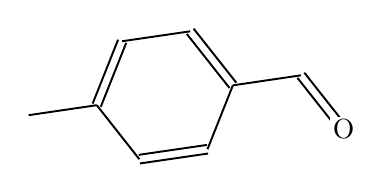
\begin{tikzpicture}[line width=.7pt]\draw (-2.000,-0.253)--(-1.135,-0.126);
\draw (-1.135,-0.126)--(-0.594,-0.812);
\draw (-0.586,-0.866)--(0.279,-0.740);
\draw (-0.602,-0.757)--(0.263,-0.631);
\draw (0.271,-0.686)--(0.594,0.126);
\draw (0.594,0.126)--(1.458,0.253);
\draw (1.415,0.219)--(1.957,-0.467);
\draw (1.501,0.287)--(2.043,-0.399);
\draw (0.637,0.160)--(0.095,0.846);
\draw (0.551,0.092)--(0.009,0.778);
\draw (0.052,0.812)--(-0.813,0.686);
\draw (-0.864,0.706)--(-1.187,-0.106);
\draw (-0.761,0.665)--(-1.084,-0.147);
\node[fill=white,inner sep=1.1pt]at(2.000,-0.433){$\mathrm{O}$};\end{tikzpicture}\par\smallskip \par\smallskip \textbf{答案（顺原空次序）：}\par\smallskip \begin{minipage}[c]{.48\linewidth}\centering (1)\par \scalebox{.83}{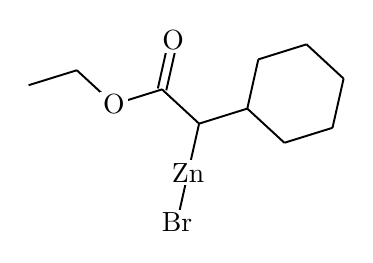
\begin{tikzpicture}[line width=.7pt]\draw (-2.000,0.583)--(-1.388,0.773);
\draw (-1.388,0.773)--(-0.917,0.339);
\draw (-0.917,0.339)--(-0.306,0.530);
\draw (-0.252,0.518)--(-0.111,1.143);
\draw (-0.359,0.542)--(-0.219,1.167);
\draw (-0.306,0.530)--(0.165,0.095);
\draw (0.165,0.095)--(0.024,-0.530);
\draw (0.024,-0.530)--(-0.116,-1.155);
\draw (0.165,0.095)--(0.777,0.286);
\draw (0.777,0.286)--(1.248,-0.148);
\draw (1.248,-0.148)--(1.859,0.042);
\draw (1.859,0.042)--(2.000,0.667);
\draw (2.000,0.667)--(1.529,1.102);
\draw (1.529,1.102)--(0.917,0.911);
\draw (0.917,0.911)--(0.777,0.286);
\node[fill=white,inner sep=1.1pt]at(-0.917,0.339){$\mathrm{O}$};
\node[fill=white,inner sep=1.1pt]at(-0.165,1.155){$\mathrm{O}$};
\node[fill=white,inner sep=1.1pt]at(0.024,-0.530){$\mathrm{Zn}$};
\node[fill=white,inner sep=1.1pt]at(-0.116,-1.155){$\mathrm{Br}$};\end{tikzpicture}}\end{minipage}\begin{minipage}[c]{.48\linewidth}\centering (2)\par \scalebox{.83}{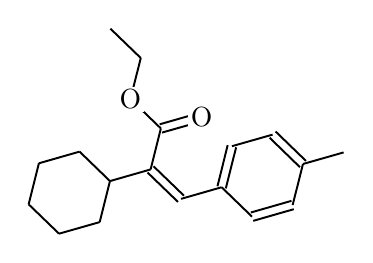
\begin{tikzpicture}[line width=.7pt]\draw (-0.962,1.302)--(-0.576,0.929);
\draw (-0.576,0.929)--(-0.707,0.408);
\draw (-0.707,0.408)--(-0.321,0.035);
\draw (-0.306,-0.018)--(0.211,0.129);
\draw (-0.336,0.087)--(0.181,0.235);
\draw (-0.321,0.035)--(-0.451,-0.486);
\draw (-0.489,-0.526)--(-0.103,-0.899);
\draw (-0.413,-0.447)--(-0.027,-0.820);
\draw (-0.065,-0.860)--(0.451,-0.712);
\draw (0.451,-0.712)--(0.837,-1.086);
\draw (0.852,-1.139)--(1.368,-0.991);
\draw (0.822,-1.033)--(1.338,-0.885);
\draw (1.353,-0.938)--(1.484,-0.417);
\draw (1.484,-0.417)--(2.000,-0.270);
\draw (1.522,-0.378)--(1.136,-0.004);
\draw (1.445,-0.457)--(1.060,-0.083);
\draw (1.098,-0.044)--(0.582,-0.191);
\draw (-0.451,-0.486)--(-0.967,-0.634);
\draw (-0.967,-0.634)--(-1.353,-0.260);
\draw (-1.353,-0.260)--(-1.870,-0.408);
\draw (-1.870,-0.408)--(-2.000,-0.929);
\draw (-2.000,-0.929)--(-1.614,-1.302);
\draw (-1.614,-1.302)--(-1.098,-1.155);
\draw (0.528,-0.178)--(0.398,-0.699);
\draw (0.635,-0.205)--(0.504,-0.726);
\draw (-1.098,-1.155)--(-0.967,-0.634);
\node[fill=white,inner sep=1.1pt]at(-0.707,0.408){$\mathrm{O}$};
\node[fill=white,inner sep=1.1pt]at(0.196,0.182){$\mathrm{O}$};\end{tikzpicture}}\end{minipage}\par\medskip\par\smallskip \textbf{推导：}锌插入$\alpha$-C—Br，第一空为$\alpha$有机锌酯（Reformatsky试剂），此时还未加入醛。它进攻对甲基苯甲醛羰基，经后处理先形成$\beta$羟基酯；原题第二步还指定酸和加热，因此进一步脱水为$\alpha$,$\beta$-不饱和酯。新双键一端连环己基与CO2Et，另一端连对甲苯基和H。\par\smallskip \par\smallskip \textbf{反校：}不能把第一空提前填$\beta$羟基酯；最终C=C不能放到环内；起料10C+醛8C=18C最终保留。\par\smallskip \par\smallskip \textbf{2分参考采分：}$\alpha$有机锌酯1分；正确脱水烯酯1分。\par\smallskip \par\smallskip \textbf{边界/原印问题：}原题未限定E/Z比例；答案连接式不指定几何，不能把任一E/Z当唯一产物。有机锌结构为教材代表式，不声称溶液只有单一单体配位态。\par\smallskip \par\smallskip 独立推导后对照本书参考答案PDF111页；有原答案缺笔处以原题碳骨架/反应守恒校正，不盲抄。\par\smallskip \par\medskip\clearpage\subsection*{15．（2分）}原书：华东理工大学模拟试题（一） 一、回答问题 第31题；PDF[108]，印刷页[103]。\par\smallskip 完成反应，填写全部原空\par\smallskip \par\smallskip 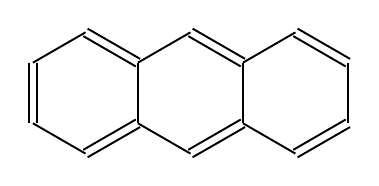
\begin{tikzpicture}[line width=.7pt]\draw (-2.055,0.385)--(-2.055,-0.385);
\draw (-1.945,0.385)--(-1.945,-0.385);
\draw (-2.000,-0.385)--(-1.333,-0.770);
\draw (-1.306,-0.817)--(-0.639,-0.433);
\draw (-1.361,-0.722)--(-0.694,-0.337);
\draw (-0.667,-0.385)--(-0.000,-0.770);
\draw (0.027,-0.817)--(0.694,-0.433);
\draw (-0.028,-0.722)--(0.639,-0.337);
\draw (0.667,-0.385)--(1.333,-0.770);
\draw (1.361,-0.817)--(2.027,-0.433);
\draw (1.306,-0.722)--(1.972,-0.337);
\draw (2.000,-0.385)--(2.000,0.385);
\draw (2.027,0.433)--(1.361,0.817);
\draw (1.972,0.337)--(1.306,0.722);
\draw (1.333,0.770)--(0.667,0.385);
\draw (0.694,0.433)--(0.028,0.817);
\draw (0.639,0.337)--(-0.027,0.722);
\draw (0.000,0.770)--(-0.667,0.385);
\draw (-0.639,0.433)--(-1.306,0.817);
\draw (-0.694,0.337)--(-1.361,0.722);
\draw (-1.333,0.770)--(-2.000,0.385);
\draw (-0.667,0.385)--(-0.667,-0.385);
\draw (0.667,0.385)--(0.667,-0.385);\end{tikzpicture}$+$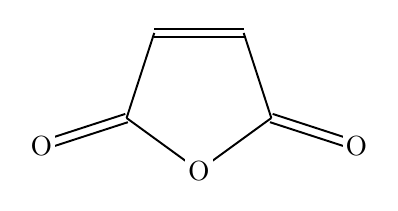
\begin{tikzpicture}[line width=.7pt]\draw (-1.983,-0.610)--(-0.902,-0.259);
\draw (-2.017,-0.505)--(-0.936,-0.154);
\draw (-0.919,-0.206)--(-0.000,-0.874);
\draw (-0.000,-0.874)--(0.919,-0.206);
\draw (0.902,-0.259)--(1.983,-0.610);
\draw (0.936,-0.154)--(2.017,-0.505);
\draw (0.919,-0.206)--(0.568,0.874);
\draw (0.568,0.929)--(-0.568,0.929);
\draw (0.568,0.819)--(-0.568,0.819);
\draw (-0.568,0.874)--(-0.919,-0.206);
\node[fill=white,inner sep=1.1pt]at(-2.000,-0.558){$\mathrm{O}$};
\node[fill=white,inner sep=1.1pt]at(-0.000,-0.874){$\mathrm{O}$};
\node[fill=white,inner sep=1.1pt]at(2.000,-0.558){$\mathrm{O}$};\end{tikzpicture}$\xrightarrow{\ \ }$（空）\par\smallskip \par\smallskip \textbf{答案（顺原空次序）：}\par\smallskip 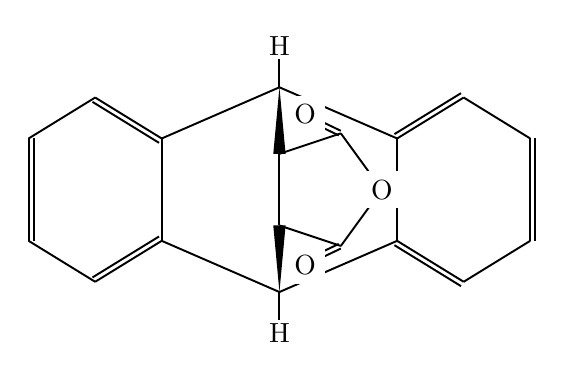
\begin{tikzpicture}[line width=.7pt]\begin{scope}[scale=.65]
\draw(0,0.7)--(0,-0.7);
\draw(0,0.7)--(1.2,1.1);
\draw(1.2,1.1)--(2,0);
\draw(2,0)--(1.2,-1.1);
\draw(1.2,-1.1)--(0,-0.7);
\draw(0,2)--(-2.3,1);
\draw(0,-2)--(-2.3,-1);
\draw(-2.3,1)--(-3.6,1.8);
\draw(-3.6,1.8)--(-4.9,1);
\draw(-4.9,1)--(-4.9,-1);
\draw(-4.9,-1)--(-3.6,-1.8);
\draw(-3.6,-1.8)--(-2.3,-1);
\draw(-2.3,-1)--(-2.3,1);
\draw(0,2)--(2.3,1);
\draw(0,-2)--(2.3,-1);
\draw(2.3,1)--(3.6,1.8);
\draw(3.6,1.8)--(4.9,1);
\draw(4.9,1)--(4.9,-1);
\draw(4.9,-1)--(3.6,-1.8);
\draw(3.6,-1.8)--(2.3,-1);
\draw(2.3,-1)--(2.3,1);
\draw(-2.3524097425664334,0.9148341683295456)--(-3.6524097425664337,1.7148341683295456);
\draw(-4.800000000000001,1.0)--(-4.800000000000001,-1.0);
\draw(-3.6524097425664337,-1.7148341683295456)--(-2.3524097425664334,-0.9148341683295456);
\draw(2.247590257433566,1.0851658316704544)--(3.5475902574335665,1.8851658316704545);
\draw(5.0,1.0)--(5.0,-1.0);
\draw(3.5475902574335665,-1.8851658316704545)--(2.247590257433566,-1.0851658316704544);
\fill(0,2)--(-.12,.7)--(.12,.7)--cycle;
\fill(0,-2)--(-.12,-.7)--(.12,-.7)--cycle;
\node[fill=white]at(2,0){$\mathrm{O}$};
\draw(1.2,1.15)--(.72,1.38);\draw(1.16,1.06)--(.68,1.29);\node[fill=white]at(.5,1.47){$\mathrm{O}$};
\draw(1.2,-1.15)--(.72,-1.38);\draw(1.16,-1.06)--(.68,-1.29);\node[fill=white]at(.5,-1.47){$\mathrm{O}$};
\draw(0,2)--(0,2.55);\node at(0,2.8){$\mathrm{H}$};\draw(0,-2)--(0,-2.55);\node at(0,-2.8){$\mathrm{H}$};
\end{scope}\end{tikzpicture}\par\smallskip \textbf{推导：}蒽中间环的9、10位作为二烯两端与顺丁烯二酸酐的双键形成两个新$\sigma$键。这样保留两个外侧苯环的芳香性；若在外侧加成则损失更多芳香稳定。亲双烯体原来的两个羰基取代部分保持顺式关系，画出9,10桥连酸酐加成物。\par\smallskip \par\smallskip \textbf{反校：}14C+4C=18C，三O均保留；不能把三个苯环全保留芳香；产物桥不等于平面四元环。\par\smallskip \par\smallskip \textbf{2分参考采分：}9/10成两新键并保留外苯环1分；顺式酸酐桥和两个羰基正确1分。\par\smallskip \par\smallskip \textbf{边界/原印问题：}原图未给独立绝对构型；图标定亲双烯体顺式关系。标准产物NIST CAS5443-16-3；不补造反应收率或endo/exo比例。\par\smallskip \par\smallskip 独立推导后对照本书参考答案PDF111页；有原答案缺笔处以原题碳骨架/反应守恒校正，不盲抄。\par\smallskip \par\medskip\clearpage\clearpage\section*{二、选择题（12题，共12分）}\subsection*{1．（1分）}\textbf{参考答案：A；D}\par\medskip{}模拟试题1·一·2\quad 印刷115页 / PDF 124页
\par\bigskip
下列烃氧基负离子碱性最弱的是（\quad），共轭酸酸性最弱的是（\quad）。
\par\bigskip
\begin{minipage}[t]{.48\linewidth}\vspace{0pt}\textbf{(A)}\par\smallskip $\mathrm{C_6H_5O^-}$\end{minipage}\hfill
\begin{minipage}[t]{.48\linewidth}\vspace{0pt}\textbf{(B)}\par\smallskip 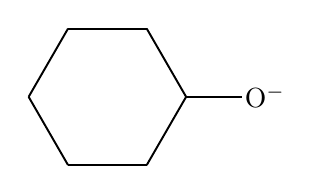
\begin{tikzpicture}[line width=.7pt,>=Stealth]
\draw (1.500,0.000)--(0.500,0.000);
\draw (0.500,0.000)--(0.000,0.866);
\draw (0.000,0.866)--(-1.000,0.866);
\draw (-1.000,0.866)--(-1.500,0.000);
\draw (-1.500,0.000)--(-1.000,-0.866);
\draw (-1.000,-0.866)--(-0.000,-0.866);
\draw (-0.000,-0.866)--(0.500,0.000);
\node[fill=white,inner sep=1.1pt]at(1.500,0.000){$\mathrm{O^{-}}$};
\end{tikzpicture}\end{minipage}\par\bigskip
\begin{minipage}[t]{.48\linewidth}\vspace{0pt}\textbf{(C)}\par\smallskip $n$-$\mathrm{C_4H_9O^-}$\end{minipage}\hfill
\begin{minipage}[t]{.48\linewidth}\vspace{0pt}\textbf{(D)}\par\smallskip $\mathrm{(CH_3)_3CO^-}$\end{minipage}\par\bigskip
\par\bigskip\textbf{教师答案：}A；D
\par\medskip\textbf{从依据到结论：}碱接受质子，酸给出质子。酚氧负离子的负电荷可向芳环离域，稳定性提高，接受质子的趋势减弱，所以第一空A。第二空独立比较共轭酸：叔丁醇在本组选项的常规教材比较中酸性最弱，所以D。
\par\medskip\textbf{选项排除：}B和C是普通醇的烷氧负离子，缺少酚氧的共振稳定；第二空不能因第一空选A而再次选A，弱碱对应较强共轭酸。
\par\medskip\textbf{反向核对及边界：}逐空核原文：两个最弱，分别比较碱和酸；不是同一性质问两遍。初录最强已用原页纠正。
\par\smallskip 本书对照：印刷118页，原答案A；D。
\par\medskip\clearpage\subsection*{2．（1分）}\textbf{参考答案：A}\par\medskip{}模拟试题8·一·6\quad 印刷159页 / PDF 168页
\par\bigskip
下列化合物中$\mathrm{S_N1}$和$\mathrm{S_N2}$都比较容易的是
\par\bigskip
\begin{minipage}[t]{.48\linewidth}\vspace{0pt}\textbf{(A)}\par\smallskip $\mathrm{PhCH_2Br}$\end{minipage}\hfill
\begin{minipage}[t]{.48\linewidth}\vspace{0pt}\textbf{(B)}\par\smallskip $\mathrm{Ph_2CHBr}$\end{minipage}\par\bigskip
\begin{minipage}[t]{.48\linewidth}\vspace{0pt}\textbf{(C)}\par\smallskip $\mathrm{PhCOCH_2Br}$\end{minipage}\hfill
\par\bigskip\textbf{教师答案：}A
\par\medskip\textbf{从依据到结论：}分别检查离解形成碳正离子的能力和背面进攻位阻。苄溴A的苄基正离子可共振稳定，且反应中心是一级碳，因而在适合各机制的条件下两种取代都容易。
\par\medskip\textbf{选项排除：}B的二苯甲基中心SN1有利但SN2位阻较大；C的羰基邻位碳适合SN2，但不能把吸电子羰基误认为稳定该处正离子的苯环。
\par\medskip\textbf{反向核对及边界：}两机制比较默认各自适宜条件；不表示同一瓶反应两机制必有相等贡献，也不声称B绝不SN2。
\par\smallskip 本书对照：印刷161页，原答案A。
\par\medskip\clearpage\subsection*{3．（1分）}\textbf{参考答案：B、C、F}\par\medskip{}模拟试题5·三·3\quad 印刷140页 / PDF 149页
\par\bigskip
下列分子哪些能进行碘仿反应？
\par\bigskip
\begin{minipage}[t]{.48\linewidth}\vspace{0pt}\textbf{(A)}\par\smallskip $\mathrm{HCHO}$\end{minipage}\hfill
\begin{minipage}[t]{.48\linewidth}\vspace{0pt}\textbf{(B)}\par\smallskip $\mathrm{CH_3CHO}$\end{minipage}\par\bigskip
\begin{minipage}[t]{.48\linewidth}\vspace{0pt}\textbf{(C)}\par\smallskip $\mathrm{(CH_3)_2CHOH}$\end{minipage}\hfill
\begin{minipage}[t]{.48\linewidth}\vspace{0pt}\textbf{(D)}\par\smallskip $\mathrm{(CH_3)_3CCHO}$\end{minipage}\par\bigskip
\begin{minipage}[t]{.48\linewidth}\vspace{0pt}\textbf{(E)}\par\smallskip $\mathrm{(CH_3CH_2)_2CHOH}$\end{minipage}\hfill
\begin{minipage}[t]{.48\linewidth}\vspace{0pt}\textbf{(F)}\par\smallskip $\mathrm{(CH_3)_2C{=}O}$\end{minipage}\par\bigskip
\par\bigskip\textbf{教师答案：}B、C、F
\par\medskip\textbf{从依据到结论：}碘仿反应识别甲基酮及能氧化为甲基酮的醇，乙醛也能发生。B是乙醛；C异丙醇先氧化为丙酮；F本身就是丙酮。
\par\medskip\textbf{选项排除：}A甲醛无所需甲基；D虽是醛，羰基旁无所需甲基；E氧化成3-戊酮，不是甲基酮。
\par\medskip\textbf{反向核对及边界：}不能只看有醇或有羰基；必须明确氧化后羰基一侧确为CH3。本题原生多选，三项都须保留。
\par\smallskip 本书对照：印刷142页，原答案B、C、F。
\par\medskip\clearpage\subsection*{4．（1分）}\textbf{参考答案：A}\par\medskip{}模拟试题8·一·1\quad 印刷158页 / PDF 167页
\par\bigskip
IUPAC的命名是
\par\bigskip
\begin{center}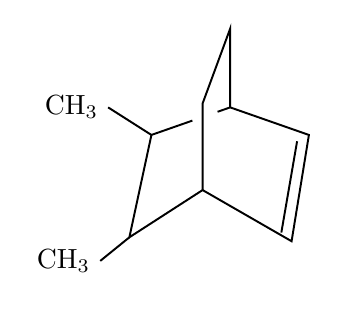
\begin{tikzpicture}[line width=.7pt,>=Stealth]
\coordinate(h1)at(0,.8);\coordinate(h2)at(-.35,-.25);\coordinate(a)at(-1,.45);\coordinate(b)at(-1.28,-.85);\coordinate(c)at(1,.45);\coordinate(d)at(.78,-.90);\coordinate(e)at(0,1.80);\coordinate(f)at(-.35,.85);
\draw(h1)--(-.16,.744);\draw(-.48,.632)--(a)--(b)--(h2)--(d)--(c)--(h1);\draw(.85,.37)--(.65,-.79);\draw(h1)--(e)--(f)--(h2);\draw(a)--(-1.55,.8)node[left]{$\mathrm{CH_3}$};\draw(b)--(-1.65,-1.15)node[left]{$\mathrm{CH_3}$};
\end{tikzpicture}\end{center}
\begin{minipage}[t]{.48\linewidth}\vspace{0pt}\textbf{(A)}\par\smallskip 5,6-二甲基二环[2.2.2]-2-辛烯\end{minipage}\hfill
\begin{minipage}[t]{.48\linewidth}\vspace{0pt}\textbf{(B)}\par\smallskip 2,3-二甲基二环[2.2.2]-5-辛烯\end{minipage}\par\bigskip
\begin{minipage}[t]{.48\linewidth}\vspace{0pt}\textbf{(C)}\par\smallskip 2,3-二甲基二环[2.2.0]-1-辛烯\end{minipage}\hfill
\begin{minipage}[t]{.48\linewidth}\vspace{0pt}\textbf{(D)}\par\smallskip 5,6-二甲基二环[2.2.2]-1-辛烯\end{minipage}\par\bigskip
\par\bigskip\textbf{教师答案：}A
\par\medskip\textbf{从依据到结论：}找到两个桥头，逐条沿不经过另一条桥的路径数中间原子，得到2、2、2，母体共2+2+2+2=8碳。优先使双键位置最低，编号为2-辛烯；两个甲基相应在5、6位。
\par\medskip\textbf{选项排除：}B让甲基先获低位，违背双键编号优先；C桥长不符；D把双键放在桥头起始位置，与原图连接关系不符。
\par\medskip\textbf{反向核对及边界：}检查桥头不算入三个括号数字；核心8碳加两个甲基总10碳。只命名原图，不额外杜撰未画立体构型。
\par\smallskip 本书对照：印刷161页，原答案A。
\par\medskip\clearpage\subsection*{5．（1分）}\textbf{参考答案：A}\par\medskip{}\subsection*{独立推导}
\par 同分子量并不保证相同分子间作用。正丙胺有N-H键，可同时作为氢键给体和受体，在自身液体中形成分子间氢键；三甲胺无N-H，虽可接受外来氢键，却不能在纯液体中提供同样的N-H氢键网络。故前者沸点明显较高。
\subsection*{各选项依据}
\par\textbf{A：}直接指出这两种纯物质最关键的相互作用差别。
\par\textbf{B：}极性可能影响沸点，但本题显著差别不应绕过N-H给体的有无。
\par\textbf{C：}形状影响色散接触，但不是本题所问主要原因。
\par\textbf{D：}描述骨架类别，没有给出为何需要更多汽化能的直接物理依据。
\subsection*{第三轮反校}
\par 三甲胺有孤对并不等于它自身可以形成N-H···N网络；题目没有比较它与水形成氢键的能力。
\par 题给46℃是原书近似差值，未另补测量温压或伪造精密数据。
\par\medskip\clearpage\subsection*{6．（1分）}\textbf{参考答案：D}\par\medskip{}\subsection*{独立推导}
\par 三者同为在相同相对位置取代的环己烷羧酸，先比较去H+后的羧酸根。经$\sigma$键的吸电子作用有利于稳定负电，给电子作用则不利。
\par F的-I吸电子效应显著；OMe中的O也有-I效应，但环中隔着饱和碳，不能用苯甲醚的直接芳香+M来抵消。Me一般给电子。课程诱导比较得到(2)>(3)>(1)。
\subsection*{各选项依据}
\par\textbf{A：}把Me取代的(1)放最强，与主要诱导方向不符。
\par\textbf{B：}把OMe放F之前，忽略两者此处主要-I强弱。
\par\textbf{C：}也把Me放最强，且把F放最弱，方向颠倒。
\par\textbf{D：}F强于OMe、OMe强于Me的本题定性结果。
\subsection*{第三轮反校}
\par 原图三者羧基与取代基相对位置均相同；未删掉中间饱和环碳，也未制造$\pi$共轭。
\par 反校比较范围：这是相近水溶条件下常规取代基趋势，不给未提供介质、cis/trans组成的精确pKa及任意条件全序。
\subsection*{适用边界}
原图没有限定cis/trans、温度与介质；定性课程结论保留，不冒称所有立体异构体/任何溶剂均有同一实测差值。
\par\medskip\clearpage\subsection*{7．（1分）}\textbf{参考答案：1}\par\medskip{}原书1.3同步练习3；印21页/PDF26页。\par 下列化合物中沸点最高的是：\par\medskip
\begin{minipage}[c][3.4cm][c]{.48\linewidth}\centering (1)\par\smallskip \scalebox{.73}{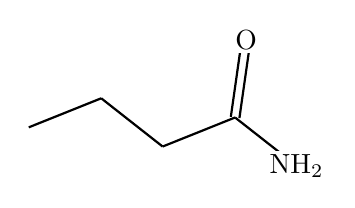
\begin{tikzpicture}[line width=.8pt]\draw (-1.700,-0.310)--(-0.780,0.059);
\draw (-0.780,0.059)--(-0.000,-0.554);
\draw (-0.000,-0.554)--(0.920,-0.185);
\draw (0.920,-0.185)--(1.700,-0.797);
\draw (0.975,-0.192)--(1.115,0.789);
\draw (0.866,-0.177)--(1.006,0.805);
\node[fill=white,inner sep=1.1pt]at(1.700,-0.797){$\mathrm{NH_{2}}$};
\node[fill=white,inner sep=1.1pt]at(1.061,0.797){$\mathrm{O}$};\end{tikzpicture}}\end{minipage}\hfill
\begin{minipage}[c][3.4cm][c]{.48\linewidth}\centering (2)\par\smallskip \scalebox{.73}{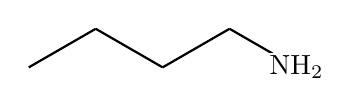
\begin{tikzpicture}[line width=.8pt]\draw (-1.700,-0.245)--(-0.850,0.245);
\draw (-0.850,0.245)--(0.000,-0.245);
\draw (0.000,-0.245)--(0.850,0.245);
\draw (0.850,0.245)--(1.700,-0.245);
\node[fill=white,inner sep=1.1pt]at(1.700,-0.245){$\mathrm{NH_{2}}$};\end{tikzpicture}}\end{minipage}\par
\begin{minipage}[c][3.4cm][c]{.48\linewidth}\centering (3)\par\smallskip \scalebox{.73}{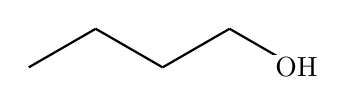
\begin{tikzpicture}[line width=.8pt]\draw (-1.700,-0.245)--(-0.850,0.245);
\draw (-0.850,0.245)--(0.000,-0.245);
\draw (0.000,-0.245)--(0.850,0.245);
\draw (0.850,0.245)--(1.700,-0.245);
\node[fill=white,inner sep=1.1pt]at(1.700,-0.245){$\mathrm{OH}$};\end{tikzpicture}}\end{minipage}\hfill
\begin{minipage}[c][3.4cm][c]{.48\linewidth}\centering (4)\par\smallskip \scalebox{.73}{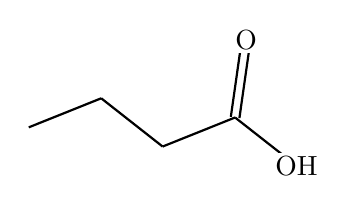
\begin{tikzpicture}[line width=.8pt]\draw (-1.700,-0.310)--(-0.780,0.059);
\draw (-0.780,0.059)--(-0.000,-0.554);
\draw (-0.000,-0.554)--(0.920,-0.185);
\draw (0.975,-0.192)--(1.115,0.789);
\draw (0.866,-0.177)--(1.006,0.805);
\draw (0.920,-0.185)--(1.700,-0.797);
\node[fill=white,inner sep=1.1pt]at(1.061,0.797){$\mathrm{O}$};
\node[fill=white,inner sep=1.1pt]at(1.700,-0.797){$\mathrm{OH}$};\end{tikzpicture}}\end{minipage}\par
\textbf{答案：}(1)。\par\textbf{从基础到判断：}四项碳数相同，首先比较官能团能产生怎样的分子间相互作用。丁酰胺既有强极性酰胺基，又可通过N—H供氢与羰基O受氢形成广泛缔合。该组中它的沸点最高，选(1)。\par\textbf{逐项核验：}\begin{enumerate}
\item 丁酰胺有强偶极及多点氢键缔合，本题最高。
\item 正丁胺能形成氢键，但胺N相关氢键通常弱于酰胺的强缔合网络，不是最高。
\item 正丁醇可形成氢键，仍低于所比丁酰胺。
\item 丁酸可形成羧酸二聚体，沸点较高，但不能因此一概压过同碳数酰胺。
\end{enumerate}\textbf{易错与边界：}先数碳确认四者都是C4系列。物性排序是特定分子间的比较，不是“所有酰胺必高于任何酸”的普遍定律。\par\smallskip 第三轮：复核否定词、原标签、逐项连接/电荷与完整共轭；独立判断后对照原书参考答案（PDF244页）一致。\par\medskip\clearpage\subsection*{8．（1分）}\textbf{参考答案：1}\par\medskip{}原书1.3同步练习6；印21页/PDF26页。\par 下列化合物中沸点最高的是：\par\medskip
\begin{minipage}[c][3.4cm][c]{.48\linewidth}\centering (1)\par\smallskip \scalebox{.73}{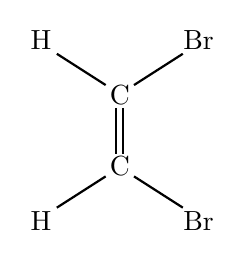
\begin{tikzpicture}[line width=.8pt]\node[fill=white,inner sep=1.1pt] at (0.000,0.450) {$\mathrm{C}$};
\node[fill=white,inner sep=1.1pt] at (0.000,-0.450) {$\mathrm{C}$};
\draw (-0.045,0.290)--(-0.045,-0.290);
\draw (0.045,0.290)--(0.045,-0.290);
\draw (-0.180,0.580)--(-0.800,0.977);
\node[fill=white,inner sep=1.1pt] at (-1.000,1.150) {$\mathrm{H}$};
\draw (0.180,0.580)--(0.800,0.977);
\node[fill=white,inner sep=1.1pt] at (1.000,1.150) {$\mathrm{Br}$};
\draw (-0.180,-0.580)--(-0.800,-0.977);
\node[fill=white,inner sep=1.1pt] at (-1.000,-1.150) {$\mathrm{H}$};
\draw (0.180,-0.580)--(0.800,-0.977);
\node[fill=white,inner sep=1.1pt] at (1.000,-1.150) {$\mathrm{Br}$};\end{tikzpicture}}\end{minipage}\hfill
\begin{minipage}[c][3.4cm][c]{.48\linewidth}\centering (2)\par\smallskip \scalebox{.73}{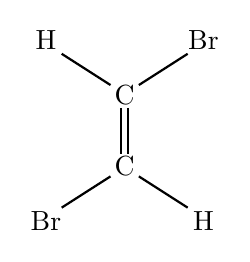
\begin{tikzpicture}[line width=.8pt]\node[fill=white,inner sep=1.1pt] at (0.000,0.450) {$\mathrm{C}$};
\node[fill=white,inner sep=1.1pt] at (0.000,-0.450) {$\mathrm{C}$};
\draw (-0.045,0.290)--(-0.045,-0.290);
\draw (0.045,0.290)--(0.045,-0.290);
\draw (-0.180,0.580)--(-0.800,0.977);
\node[fill=white,inner sep=1.1pt] at (-1.000,1.150) {$\mathrm{H}$};
\draw (0.180,0.580)--(0.800,0.977);
\node[fill=white,inner sep=1.1pt] at (1.000,1.150) {$\mathrm{Br}$};
\draw (-0.180,-0.580)--(-0.800,-0.977);
\node[fill=white,inner sep=1.1pt] at (-1.000,-1.150) {$\mathrm{Br}$};
\draw (0.180,-0.580)--(0.800,-0.977);
\node[fill=white,inner sep=1.1pt] at (1.000,-1.150) {$\mathrm{H}$};\end{tikzpicture}}\end{minipage}\par
\begin{minipage}[c][3.4cm][c]{.48\linewidth}\centering (3)\par\smallskip \scalebox{.73}{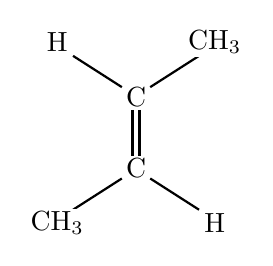
\begin{tikzpicture}[line width=.8pt]\node[fill=white,inner sep=1.1pt] at (0.000,0.450) {$\mathrm{C}$};
\node[fill=white,inner sep=1.1pt] at (0.000,-0.450) {$\mathrm{C}$};
\draw (-0.045,0.290)--(-0.045,-0.290);
\draw (0.045,0.290)--(0.045,-0.290);
\draw (-0.180,0.580)--(-0.800,0.977);
\node[fill=white,inner sep=1.1pt] at (-1.000,1.150) {$\mathrm{H}$};
\draw (0.180,0.580)--(0.800,0.977);
\node[fill=white,inner sep=1.1pt] at (1.000,1.150) {$\mathrm{CH_3}$};
\draw (-0.180,-0.580)--(-0.800,-0.977);
\node[fill=white,inner sep=1.1pt] at (-1.000,-1.150) {$\mathrm{CH_3}$};
\draw (0.180,-0.580)--(0.800,-0.977);
\node[fill=white,inner sep=1.1pt] at (1.000,-1.150) {$\mathrm{H}$};\end{tikzpicture}}\end{minipage}\hfill
\begin{minipage}[c][3.4cm][c]{.48\linewidth}\centering (4)\par\smallskip \scalebox{.73}{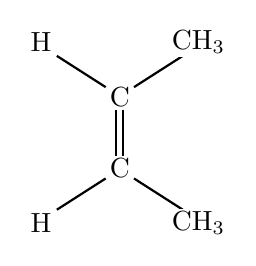
\begin{tikzpicture}[line width=.8pt]\node[fill=white,inner sep=1.1pt] at (0.000,0.450) {$\mathrm{C}$};
\node[fill=white,inner sep=1.1pt] at (0.000,-0.450) {$\mathrm{C}$};
\draw (-0.045,0.290)--(-0.045,-0.290);
\draw (0.045,0.290)--(0.045,-0.290);
\draw (-0.180,0.580)--(-0.800,0.977);
\node[fill=white,inner sep=1.1pt] at (-1.000,1.150) {$\mathrm{H}$};
\draw (0.180,0.580)--(0.800,0.977);
\node[fill=white,inner sep=1.1pt] at (1.000,1.150) {$\mathrm{CH_3}$};
\draw (-0.180,-0.580)--(-0.800,-0.977);
\node[fill=white,inner sep=1.1pt] at (-1.000,-1.150) {$\mathrm{H}$};
\draw (0.180,-0.580)--(0.800,-0.977);
\node[fill=white,inner sep=1.1pt] at (1.000,-1.150) {$\mathrm{CH_3}$};\end{tikzpicture}}\end{minipage}\par
\textbf{答案：}(1)。\par\textbf{从基础到判断：}先分清同分异构体：图(1)(2)为顺/反1,2-二溴乙烯，(3)(4)为反/顺2-丁烯。溴原子较大、可极化性强，使前两项的色散作用远强于丁烯；再比较同分子式的顺反异构体。顺式的键偶极不能像反式那样抵消，其液体分子间吸引更强，本组最高为(1)。\par\textbf{逐项核验：}\begin{enumerate}
\item 两Br在双键同侧，为顺式二溴乙烯；本组沸点最高。
\item 反式二溴乙烯的分子对称性使偶极抵消，低于顺式。
\item 反2-丁烯，没有Br，色散作用较弱，不选。
\item 顺2-丁烯虽有净偶极，仍不能超过较重二溴乙烯，不选。
\end{enumerate}\textbf{易错与边界：}对同系列用偶极解释沸点，不能把反式较易堆积的熔点规律搬到沸点。此题保留原四项顺反画法，未交换左右标签。\par\smallskip 第三轮：复核否定词、原标签、逐项连接/电荷与完整共轭；独立判断后对照原书参考答案（PDF244页）一致。\par\medskip\clearpage\subsection*{9．（1分）}\textbf{参考答案：4}\par\medskip{}原书1.3同步练习4；印21页/PDF26页。\par 下列化合物中沸点最低的是：\par\medskip
\begin{minipage}[c][3.4cm][c]{.48\linewidth}\centering (1)\par\smallskip \scalebox{.73}{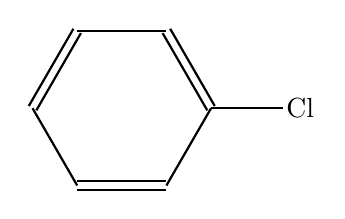
\begin{tikzpicture}[line width=.8pt]\draw (1.700,0.000)--(0.567,0.000);
\draw (0.614,0.028)--(0.048,1.009);
\draw (0.519,-0.027)--(-0.048,0.954);
\draw (0.000,0.981)--(-1.133,0.981);
\draw (-1.181,1.009)--(-1.748,0.028);
\draw (-1.086,0.954)--(-1.652,-0.027);
\draw (-1.700,0.000)--(-1.133,-0.981);
\draw (-1.133,-1.036)--(-0.000,-1.036);
\draw (-1.133,-0.926)--(-0.000,-0.926);
\draw (-0.000,-0.981)--(0.567,0.000);
\node[fill=white,inner sep=1.1pt]at(1.700,0.000){$\mathrm{Cl}$};\end{tikzpicture}}\end{minipage}\hfill
\begin{minipage}[c][3.4cm][c]{.48\linewidth}\centering (2)\par\smallskip \scalebox{.73}{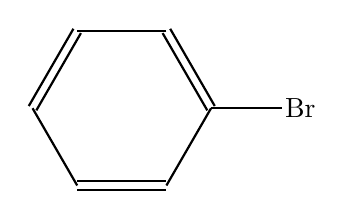
\begin{tikzpicture}[line width=.8pt]\draw (1.700,0.000)--(0.567,0.000);
\draw (0.614,0.028)--(0.048,1.009);
\draw (0.519,-0.027)--(-0.048,0.954);
\draw (0.000,0.981)--(-1.133,0.981);
\draw (-1.181,1.009)--(-1.748,0.028);
\draw (-1.086,0.954)--(-1.652,-0.027);
\draw (-1.700,0.000)--(-1.133,-0.981);
\draw (-1.133,-1.036)--(-0.000,-1.036);
\draw (-1.133,-0.926)--(-0.000,-0.926);
\draw (-0.000,-0.981)--(0.567,0.000);
\node[fill=white,inner sep=1.1pt]at(1.700,0.000){$\mathrm{Br}$};\end{tikzpicture}}\end{minipage}\par
\begin{minipage}[c][3.4cm][c]{.48\linewidth}\centering (3)\par\smallskip \scalebox{.73}{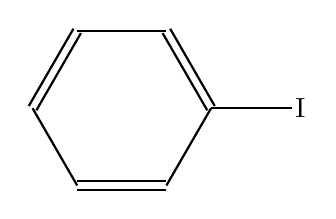
\begin{tikzpicture}[line width=.8pt]\draw (1.700,0.000)--(0.567,0.000);
\draw (0.614,0.028)--(0.048,1.009);
\draw (0.519,-0.027)--(-0.048,0.954);
\draw (0.000,0.981)--(-1.133,0.981);
\draw (-1.181,1.009)--(-1.748,0.028);
\draw (-1.086,0.954)--(-1.652,-0.027);
\draw (-1.700,0.000)--(-1.133,-0.981);
\draw (-1.133,-1.036)--(-0.000,-1.036);
\draw (-1.133,-0.926)--(-0.000,-0.926);
\draw (-0.000,-0.981)--(0.567,0.000);
\node[fill=white,inner sep=1.1pt]at(1.700,0.000){$\mathrm{I}$};\end{tikzpicture}}\end{minipage}\hfill
\begin{minipage}[c][3.4cm][c]{.48\linewidth}\centering (4)\par\smallskip \scalebox{.73}{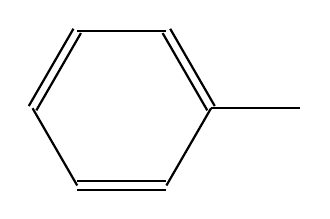
\begin{tikzpicture}[line width=.8pt]\draw (1.700,0.000)--(0.567,0.000);
\draw (0.614,0.028)--(0.048,1.009);
\draw (0.519,-0.027)--(-0.048,0.954);
\draw (0.000,0.981)--(-1.133,0.981);
\draw (-1.181,1.009)--(-1.748,0.028);
\draw (-1.086,0.954)--(-1.652,-0.027);
\draw (-1.700,0.000)--(-1.133,-0.981);
\draw (-1.133,-1.036)--(-0.000,-1.036);
\draw (-1.133,-0.926)--(-0.000,-0.926);
\draw (-0.000,-0.981)--(0.567,0.000);\end{tikzpicture}}\end{minipage}\par
\textbf{答案：}(4)。\par\textbf{从基础到判断：}先识别前三项依次为氯苯、溴苯、碘苯，第四为甲苯。它们都没有能形成强分子间氢键的供氢官能团；主要比较色散与偶极作用。所列卤代苯比甲苯的沸点高，卤素从Cl到I可极化性总体增加。最低为甲苯(4)。\par\textbf{逐项核验：}\begin{enumerate}
\item 氯苯有较强可极化的C—Cl相关分子间作用，不是最低。
\item 溴苯电子云更易极化，不选。
\item 碘苯色散作用强，不选。
\item 甲苯在这四个具体化合物中沸点最低，选。
\end{enumerate}\textbf{易错与边界：}不能用“极性更大所以一定沸点更高”代替全部比较；也不能把相对分子质量单独当作放之四海皆准的排序法。\par\smallskip 第三轮：复核否定词、原标签、逐项连接/电荷与完整共轭；独立判断后对照原书参考答案（PDF244页）一致。\par\medskip\clearpage\subsection*{10．（1分）}\textbf{参考答案：A、C、D}\par\medskip{}模拟试题5·三·2\quad 印刷140页 / PDF 149页
\par\bigskip
下列分子或基团中哪些具有芳香性？
\par\bigskip
\begin{minipage}[t]{.48\linewidth}\vspace{0pt}\textbf{(A)}\par\smallskip 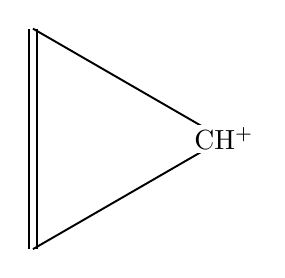
\begin{tikzpicture}[line width=.7pt,>=Stealth]
\draw (1.212,-0.000)--(-1.212,1.400);
\draw (-1.267,1.400)--(-1.267,-1.400);
\draw (-1.157,1.400)--(-1.157,-1.400);
\draw (-1.212,-1.400)--(1.212,-0.000);
\node[fill=white,inner sep=1.1pt]at(1.212,-0.000){$\mathrm{CH^{+}}$};
\end{tikzpicture}\end{minipage}\hfill
\begin{minipage}[t]{.48\linewidth}\vspace{0pt}\textbf{(B)}\par\smallskip 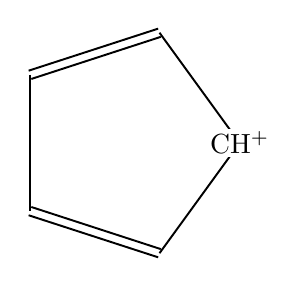
\begin{tikzpicture}[line width=.7pt,>=Stealth]
\draw (1.331,0.000)--(0.314,1.400);
\draw (0.297,1.452)--(-1.348,0.918);
\draw (0.331,1.348)--(-1.314,0.813);
\draw (-1.331,0.865)--(-1.331,-0.865);
\draw (-1.348,-0.918)--(0.297,-1.452);
\draw (-1.314,-0.813)--(0.331,-1.348);
\draw (0.314,-1.400)--(1.331,0.000);
\node[fill=white,inner sep=1.1pt]at(1.331,0.000){$\mathrm{CH^{+}}$};
\end{tikzpicture}\end{minipage}\par\bigskip
\begin{minipage}[t]{.48\linewidth}\vspace{0pt}\textbf{(C)}\par\smallskip 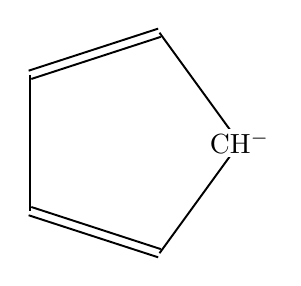
\begin{tikzpicture}[line width=.7pt,>=Stealth]
\draw (1.331,0.000)--(0.314,1.400);
\draw (0.297,1.452)--(-1.348,0.918);
\draw (0.331,1.348)--(-1.314,0.813);
\draw (-1.331,0.865)--(-1.331,-0.865);
\draw (-1.348,-0.918)--(0.297,-1.452);
\draw (-1.314,-0.813)--(0.331,-1.348);
\draw (0.314,-1.400)--(1.331,0.000);
\node[fill=white,inner sep=1.1pt]at(1.331,0.000){$\mathrm{CH^{-}}$};
\end{tikzpicture}\end{minipage}\hfill
\begin{minipage}[t]{.48\linewidth}\vspace{0pt}\textbf{(D)}\par\smallskip 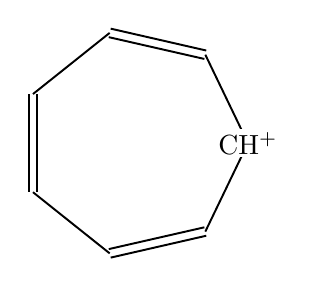
\begin{tikzpicture}[line width=.7pt,>=Stealth]
\draw (1.365,-0.000)--(0.824,1.123);
\draw (0.836,1.176)--(-0.378,1.454);
\draw (0.812,1.069)--(-0.403,1.346);
\draw (-0.391,1.400)--(-1.365,0.623);
\draw (-1.420,0.623)--(-1.420,-0.623);
\draw (-1.310,0.623)--(-1.310,-0.623);
\draw (-1.365,-0.623)--(-0.391,-1.400);
\draw (-0.378,-1.454)--(0.836,-1.176);
\draw (-0.403,-1.346)--(0.812,-1.069);
\draw (0.824,-1.123)--(1.365,-0.000);
\node[fill=white,inner sep=1.1pt]at(1.365,-0.000){$\mathrm{CH^{+}}$};
\end{tikzpicture}\end{minipage}\par\bigskip
\begin{minipage}[t]{.48\linewidth}\vspace{0pt}\textbf{(E)}\par\smallskip 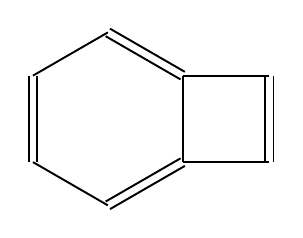
\begin{tikzpicture}[line width=.7pt,>=Stealth]
\draw (-1.500,-0.549)--(-0.549,-1.098);
\draw (-0.522,-1.146)--(0.429,-0.597);
\draw (-0.577,-1.050)--(0.374,-0.501);
\draw (0.402,-0.549)--(0.402,0.549);
\draw (0.429,0.597)--(-0.522,1.146);
\draw (0.374,0.501)--(-0.577,1.050);
\draw (-0.549,1.098)--(-1.500,0.549);
\draw (0.402,0.549)--(1.500,0.549);
\draw (1.445,0.549)--(1.445,-0.549);
\draw (1.555,0.549)--(1.555,-0.549);
\draw (-1.555,0.549)--(-1.555,-0.549);
\draw (-1.445,0.549)--(-1.445,-0.549);
\draw (1.500,-0.549)--(0.402,-0.549);
\end{tikzpicture}\end{minipage}\hfill
\par\bigskip\textbf{教师答案：}A、C、D
\par\medskip\textbf{从依据到结论：}芳香性要求环状连续共轭、可近似平面且具有4n+2个$\pi$电子。A环丙烯正离子2$\pi$；C环戊二烯负离子6$\pi$；D环庚三烯正离子6$\pi$，均符合。
\par\medskip\textbf{选项排除：}B环戊二烯正离子为4$\pi$，不符合芳香稳定条件；E苯并环丁二烯不能因局部画了苯环就把整个稠合体系判为题目要求的芳香体系。
\par\medskip\textbf{反向核对及边界：}先核电荷再数电子：负碳孤对贡献2，正碳空p贡献0；不要把多环总电子计数法无条件套在任何稠环上。E按本书整体体系题意排除，不否认局部芳香性讨论。
\par\smallskip 本书对照：印刷142页，原答案A、C、D。
\par\medskip\clearpage\subsection*{11．（1分）}\textbf{参考答案：B}\par\medskip{}\subsection*{独立推导}
\par 原题两个桥头H均为实楔，首先固定cis稠合，Me也在所标同侧。翻椅不能把cis稠合变成trans。
\par 在同一椅式环的相邻两个桥头上，cis稠合需要另一环的连接一轴一赤道，另一环因此相对折起。B保留该cis稠合，并把相应Me放到有利的赤道位置；不能只看某幅图横着画、Me像平伏就选。
\subsection*{各选项依据}
\par\textbf{A：}原A的平展轮廓不是题示cis稠合的相应稳定椅—椅安排；只保留Me平伏不足。
\par\textbf{B：}相对折起的两个椅式符合cis公共键两端关系，且Me取向与原图一致。
\par\textbf{C：}改变Me朝向不能补救其稠合骨架与原图的关系不符。
\par\textbf{D：}同样不能仅用末端Me看似平伏判优，须先满足原桥头cis关系。
\subsection*{第三轮反校}
\par 重新从两个桥头逐端追踪H：必须同面，不用整图旋转把一端H翻到反面。
\par 两环共用2C和1键，总环C为10；正式图是手工空间矢量，不把平面连接图当椅式证明。
\begin{center}\resizebox{.35\linewidth}{!}{\begin{tikzpicture}[line width=.8pt,>=Stealth,baseline=(current bounding box.center)]
\draw[](-1.414,-0.9520000000000001)--(-1.19,-0.112);
\draw[](-1.19,-0.112)--(-0.294,-0.336);
\draw[](-0.294,-0.336)--(0.546,-0.0);
\draw[](0.546,-0.0)--(0.406,-1.204);
\draw[line width=1.8pt](0.406,-1.204)--(-0.462,-1.12);
\draw[](-0.462,-1.12)--(-1.414,-0.9520000000000001);
\draw[](0.546,-0.0)--(0.546,0.7000000000000001);
\draw[](0.546,0.7000000000000001)--(1.414,1.204);
\draw[](1.414,1.204)--(1.078,0.084);
\draw[line width=1.8pt](1.078,0.084)--(1.05,-0.9520000000000001);
\draw[line width=1.8pt](1.05,-0.9520000000000001)--(0.406,-1.204);\draw[](1.078,0.084)--(1.8900000000000001,0.364);\node[anchor=west,fill=white,inner sep=1pt]at(2.1100000000000003,0.364){$\mathrm{CH_3}$};
\end{tikzpicture}}\end{center}
\par 核对入口：\url{https://openstax.org/books/organic-chemistry/pages/4-9-conformations-of-polycyclic-molecules}
\par\medskip\clearpage\subsection*{12．（1分）}\textbf{参考答案：D}\par\medskip{}模拟试题8·一·9\quad 印刷159页 / PDF 168页
\par\bigskip
下列4种溶剂相对密度大于1的是
\par\bigskip
\begin{minipage}[t]{.48\linewidth}\vspace{0pt}\textbf{(A)}\par\smallskip 正庚烷\end{minipage}\hfill
\begin{minipage}[t]{.48\linewidth}\vspace{0pt}\textbf{(B)}\par\smallskip 环己烷\end{minipage}\par\bigskip
\begin{minipage}[t]{.48\linewidth}\vspace{0pt}\textbf{(C)}\par\smallskip 乙醚\end{minipage}\hfill
\begin{minipage}[t]{.48\linewidth}\vspace{0pt}\textbf{(D)}\par\smallskip 1,2-二氯乙烷\end{minipage}\par\bigskip
\par\bigskip\textbf{教师答案：}D
\par\medskip\textbf{从依据到结论：}相对密度以水为比较对象。常温教材所列正庚烷、环己烷及乙醚均小于水；含两个氯的1,2-二氯乙烷密度大于水，因此选D。
\par\medskip\textbf{选项排除：}A、B、C不能因为是有机液体就一概判断密度大于1；卤代物也并非全部大于1，应结合具体分子。
\par\medskip\textbf{反向核对及边界：}本题不要求虚构精确密度；仅比较原选项的常温液体与水。温度未标时按通常物性表范围解读。
\par\smallskip 本书对照：印刷161页，原答案D。
\par\medskip\clearpage\clearpage\section*{三、结构推导（5题，共35分）}\subsection*{1．（8分）}(A)分子式为$\mathrm{C_{15}H_{24}}$，催化氢化吸收4 mol $\mathrm H_2$，得到下示饱和烃。(A)先用臭氧处理，后用Zn和$\mathrm{H_2O}$处理，得两分子甲醛、一分子丙酮、一分子$\mathrm{CH_3COCH_2CH_2CHO}$和一分子$\mathrm{OHCCH_2CH_2COCHO}$。不管其顺反异构，写出构造式。
\begin{center}\resizebox{.50\linewidth}{!}{\begin{tikzpicture}[line width=.8pt,>=Stealth,baseline=(current bounding box.center)]
\draw (-2.000,-0.373)--(-1.530,-0.379);
\draw (-1.530,-0.379)--(-1.300,-0.789);
\draw (-1.530,-0.379)--(-1.290,0.025);
\draw (-1.290,0.025)--(-0.820,0.020);
\draw (-0.820,0.020)--(-0.580,0.424);
\draw (-0.580,0.424)--(-0.110,0.418);
\draw (-0.110,0.418)--(0.130,0.822);
\draw (-0.110,0.418)--(0.120,0.008);
\draw (0.120,0.008)--(0.590,0.003);
\draw (0.590,0.003)--(0.820,-0.407);
\draw (0.820,-0.407)--(1.290,-0.413);
\draw (1.290,-0.413)--(1.520,-0.822);
\draw (1.290,-0.413)--(1.530,-0.008);
\draw (1.530,-0.008)--(2.000,-0.014);
\node at(0.0,-1.7){$\mathrm{hydrogenation}$};
\draw (4.400,-0.055)--(7.200,-0.055);
\draw (4.400,0.055)--(7.200,0.055);
\node[fill=white,inner sep=1.1pt]at(7.200,-0.000){$\mathrm{O}$};
\node at(5.8,-1.7){$\mathrm{2 mol}$};
\draw (-1.617,-5.200)--(0.000,-4.267);
\draw (0.000,-4.267)--(1.617,-5.200);
\draw (0.055,-4.267)--(0.055,-2.400);
\draw (-0.055,-4.267)--(-0.055,-2.400);
\node[fill=white,inner sep=1.1pt]at(0.000,-2.400){$\mathrm{O}$};
\node at(0.0,-5.5){$\mathrm{1 mol}$};
\draw (7.800,-3.079)--(7.021,-3.591);
\draw (6.966,-3.594)--(7.020,-4.524);
\draw (7.076,-3.588)--(7.130,-4.517);
\draw (7.021,-3.591)--(6.189,-3.172);
\draw (6.189,-3.172)--(5.411,-3.683);
\draw (5.411,-3.683)--(4.579,-3.265);
\draw (4.548,-3.219)--(3.770,-3.730);
\draw (4.609,-3.311)--(3.830,-3.822);
\node[fill=white,inner sep=1.1pt]at(7.075,-4.521){$\mathrm{O}$};
\node[fill=white,inner sep=1.1pt]at(3.800,-3.776){$\mathrm{O}$};
\node at(5.8,-5.5){$\mathrm{1 mol}$};
\draw (-2.030,-7.701)--(-1.381,-8.116);
\draw (-1.970,-7.608)--(-1.321,-8.024);
\draw (-1.351,-8.070)--(-0.667,-7.716);
\draw (-0.667,-7.716)--(-0.018,-8.131);
\draw (-0.018,-8.131)--(0.667,-7.777);
\draw (0.722,-7.780)--(0.757,-7.010);
\draw (0.612,-7.775)--(0.647,-7.005);
\draw (0.667,-7.777)--(1.316,-8.193);
\draw (1.341,-8.242)--(2.025,-7.887);
\draw (1.290,-8.144)--(1.975,-7.790);
\node[fill=white,inner sep=1.1pt]at(-2.000,-7.654){$\mathrm{O}$};
\node[fill=white,inner sep=1.1pt]at(0.702,-7.007){$\mathrm{O}$};
\node[fill=white,inner sep=1.1pt]at(2.000,-7.839){$\mathrm{O}$};
\node at(0.0,-9.299999999999999){$\mathrm{1 mol}$};
\end{tikzpicture}}\end{center}
\subsection*{答案与边界}
符合全部条件的一式为$\mathrm{CH_2=CHC(=CH_2)CH_2CH_2CH=C(CH_3)CH_2CH_2CH=C(CH_3)_2}$（E/Z不指定）。
\begin{center}\resizebox{.50\linewidth}{!}{\begin{tikzpicture}[line width=.8pt,>=Stealth,baseline=(current bounding box.center)]
\draw (1.954,0.651)--(1.677,0.242);
\draw (2.046,0.589)--(1.768,0.180);
\draw (1.723,0.211)--(1.231,0.247);
\draw (1.280,0.271)--(1.065,0.715);
\draw (1.181,0.223)--(0.966,0.667);
\draw (1.231,0.247)--(0.953,-0.161);
\draw (0.953,-0.161)--(0.461,-0.125);
\draw (0.461,-0.125)--(0.184,-0.534);
\draw (0.188,-0.479)--(-0.304,-0.443);
\draw (0.180,-0.589)--(-0.312,-0.553);
\draw (-0.308,-0.498)--(-0.585,-0.906);
\draw (-0.308,-0.498)--(-0.523,-0.054);
\draw (-0.523,-0.054)--(-1.016,-0.018);
\draw (-1.016,-0.018)--(-1.231,0.426);
\draw (-1.227,0.481)--(-1.719,0.517);
\draw (-1.235,0.371)--(-1.727,0.407);
\draw (-1.723,0.462)--(-1.938,0.906);
\draw (-1.723,0.462)--(-2.000,0.054);
\node at(0.0,-1.7){$\mathrm{}$};
\end{tikzpicture}}\end{center}
\subsection*{独立推导}
\par DBE=4且完全加4H2，按常规模型为开链四烯；题给氢化后支链骨架必须保留。
\par 两个甲醛指向两处末端=CH2；丙酮指向一端=(CH3)2C。两个五碳片段的羰基间碳距分别给出剩余端点连接约束，其中相邻二羰基片段锁定共轭局部。
\par 沿题给2,6,10-三甲基十二烷骨架逐端回接，得到答图四烯；不能只凑C15H24而忽略氢化骨架。
\subsection*{第三轮化学反校}
\par 逐条切四个C=C，实际给2甲醛+丙酮+CH3COCH2CH2CHO+OHCCH2CH2COCHO；碳2+3+5+5=15。
\par 把所有C=C还原为单键，结构与题给支链间隔一致。羰基端配对枚举仅作辅助，不能替代这两条化学回代。
\par 原解析另列构造式的氢化支链间隔与题给不合，不照抄该式，不擅自改变题给氢化产物。
\subsection*{参考采分点（编辑建议）}
\par 下列为编辑建议，非原书官方评分。
\par 8分：DBE1；末端/丙酮1；五碳片段2；完整四烯2；氢化骨架回代2。
\par\vspace{3mm}\footnotesize 来源：S01；PDF 156；印刷 150；题号8-65。\normalsize
\par\medskip\clearpage\subsection*{2．（8分）}芳香化合物A、B、C分子式均为$\mathrm{C_{10}H_{14}}$，$^1\mathrm H$ NMR图谱如下。确定结构并指出各氢在谱上的归属。
\textbf{A}\begin{center}\resizebox{.87\linewidth}{!}{\begin{tikzpicture}[line width=.8pt,>=Stealth,baseline=(current bounding box.center)]
\draw(0,0)--(12,0);
\draw(12.0,0)--(12.0,-.12)node[below]{$0$};
\draw(10.5,0)--(10.5,-.12)node[below]{$1$};
\draw(9.0,0)--(9.0,-.12)node[below]{$2$};
\draw(7.5,0)--(7.5,-.12)node[below]{$3$};
\draw(6.0,0)--(6.0,-.12)node[below]{$4$};
\draw(4.5,0)--(4.5,-.12)node[below]{$5$};
\draw(3.0,0)--(3.0,-.12)node[below]{$6$};
\draw(1.5,0)--(1.5,-.12)node[below]{$7$};
\draw(0.0,0)--(0.0,-.12)node[below]{$8$};
\node at(6,-1.5){$\delta$};
\draw[blue!60!black,line width=.5pt](1.4550000000000003,0)--(1.4550000000000003,2.3);
\draw[blue!60!black,line width=.5pt](1.3950000000000002,0)--(1.3950000000000002,2.3);
\draw[blue!60!black,line width=.5pt](1.3350000000000002,0)--(1.3350000000000002,2.3);
\draw[blue!60!black,line width=.5pt](1.2750000000000001,0)--(1.2750000000000001,2.3);
\draw[red!50!black](1.1150000000000002,0.2)--(1.3050000000000002,0.2)--(1.4150000000000003,0.6000000000000001)--(1.6650000000000003,0.6000000000000001);
\draw[blue!60!black,line width=.5pt](7.822500000000002,0)--(7.822500000000002,0.025);
\draw[blue!60!black,line width=.5pt](7.785,0)--(7.785,0.15);
\draw[blue!60!black,line width=.5pt](7.747500000000001,0)--(7.747500000000001,0.375);
\draw[blue!60!black,line width=.5pt](7.710000000000001,0)--(7.710000000000001,0.5);
\draw[blue!60!black,line width=.5pt](7.6725,0)--(7.6725,0.375);
\draw[blue!60!black,line width=.5pt](7.635000000000002,0)--(7.635000000000002,0.15);
\draw[blue!60!black,line width=.5pt](7.5975,0)--(7.5975,0.025);
\draw[red!50!black](7.460000000000001,0.6000000000000001)--(7.650000000000001,0.6000000000000001)--(7.760000000000001,0.7)--(8.010000000000002,0.7);
\draw[blue!60!black,line width=.5pt](8.715,0)--(8.715,1.4);
\draw[red!50!black](8.465,0.7)--(8.655,0.7)--(8.765,1.0)--(9.015,1.0);
\draw[blue!60!black,line width=.5pt](10.2675,0)--(10.2675,1.8);
\draw[blue!60!black,line width=.5pt](10.1325,0)--(10.1325,1.8);
\draw[red!50!black](9.95,1.0)--(10.139999999999999,1.0)--(10.25,1.6)--(10.5,1.6);
\draw[blue!60!black,line width=.45pt](11.92,0)--(11.95,0)--(11.97,0.55)--(11.99,0)--(12.02,0);
\end{tikzpicture}}\end{center}\par\textbf{B}\begin{center}\resizebox{.87\linewidth}{!}{\begin{tikzpicture}[line width=.8pt,>=Stealth,baseline=(current bounding box.center)]
\draw(0,0)--(12,0);
\draw(12.0,0)--(12.0,-.12)node[below]{$0$};
\draw(10.5,0)--(10.5,-.12)node[below]{$1$};
\draw(9.0,0)--(9.0,-.12)node[below]{$2$};
\draw(7.5,0)--(7.5,-.12)node[below]{$3$};
\draw(6.0,0)--(6.0,-.12)node[below]{$4$};
\draw(4.5,0)--(4.5,-.12)node[below]{$5$};
\draw(3.0,0)--(3.0,-.12)node[below]{$6$};
\draw(1.5,0)--(1.5,-.12)node[below]{$7$};
\draw(0.0,0)--(0.0,-.12)node[below]{$8$};
\node at(6,-1.5){$\delta$};
\draw[blue!60!black,line width=.5pt](1.1400000000000001,0)--(1.1400000000000001,0.09999999999999999);
\draw[blue!60!black,line width=.5pt](1.0650000000000004,0)--(1.0650000000000004,0.19999999999999998);
\draw[blue!60!black,line width=.5pt](0.9900000000000002,0)--(0.9900000000000002,0.3);
\draw[blue!60!black,line width=.5pt](0.9150000000000001,0)--(0.9150000000000001,0.19999999999999998);
\draw[blue!60!black,line width=.5pt](0.8400000000000003,0)--(0.8400000000000003,0.09999999999999999);
\draw[red!50!black](0.7400000000000002,0.2)--(0.9300000000000002,0.2)--(1.0400000000000003,0.7)--(1.2900000000000003,0.7);
\draw[blue!60!black,line width=.5pt](9.975000000000001,0)--(9.975000000000001,3.0);
\draw[red!50!black](9.725000000000001,0.7)--(9.915000000000001,0.7)--(10.025000000000002,1.6)--(10.275000000000002,1.6);
\draw[blue!60!black,line width=.45pt](11.92,0)--(11.95,0)--(11.97,0.08)--(11.99,0)--(12.02,0);
\end{tikzpicture}}\end{center}\par\textbf{C}\begin{center}\resizebox{.87\linewidth}{!}{\begin{tikzpicture}[line width=.8pt,>=Stealth,baseline=(current bounding box.center)]
\draw(0,0)--(12,0);
\draw(12.0,0)--(12.0,-.12)node[below]{$0$};
\draw(10.5,0)--(10.5,-.12)node[below]{$1$};
\draw(9.0,0)--(9.0,-.12)node[below]{$2$};
\draw(7.5,0)--(7.5,-.12)node[below]{$3$};
\draw(6.0,0)--(6.0,-.12)node[below]{$4$};
\draw(4.5,0)--(4.5,-.12)node[below]{$5$};
\draw(3.0,0)--(3.0,-.12)node[below]{$6$};
\draw(1.5,0)--(1.5,-.12)node[below]{$7$};
\draw(0.0,0)--(0.0,-.12)node[below]{$8$};
\node at(6,-1.5){$\delta$};
\draw[blue!60!black,line width=.5pt](1.305,0)--(1.305,0.7333333333333334);
\draw[blue!60!black,line width=.5pt](1.245,0)--(1.245,1.4666666666666668);
\draw[blue!60!black,line width=.5pt](1.185,0)--(1.185,2.2);
\draw[blue!60!black,line width=.5pt](1.125,0)--(1.125,1.4666666666666668);
\draw[blue!60!black,line width=.5pt](1.0650000000000002,0)--(1.0650000000000002,0.7333333333333334);
\draw[red!50!black](0.935,0.2)--(1.125,0.2)--(1.235,0.7)--(1.485,0.7);
\draw[blue!60!black,line width=.5pt](8.415000000000001,0)--(8.415000000000001,0.7);
\draw[blue!60!black,line width=.5pt](8.295,0)--(8.295,0.7);
\draw[red!50!black](8.105,0.7)--(8.295,0.7)--(8.405000000000001,0.9000000000000001)--(8.655000000000001,0.9000000000000001);
\draw[blue!60!black,line width=.5pt](9.45,0)--(9.45,0.05714285714285715);
\draw[blue!60!black,line width=.5pt](9.39,0)--(9.39,0.17142857142857146);
\draw[blue!60!black,line width=.5pt](9.33,0)--(9.33,0.2857142857142857);
\draw[blue!60!black,line width=.5pt](9.27,0)--(9.27,0.4);
\draw[blue!60!black,line width=.5pt](9.209999999999999,0)--(9.209999999999999,0.2857142857142857);
\draw[blue!60!black,line width=.5pt](9.149999999999999,0)--(9.149999999999999,0.17142857142857146);
\draw[blue!60!black,line width=.5pt](9.09,0)--(9.09,0.05714285714285715);
\draw[red!50!black](9.02,0.9000000000000001)--(9.209999999999999,0.9000000000000001)--(9.32,1.0)--(9.57,1.0);
\draw[blue!60!black,line width=.5pt](10.7625,0)--(10.7625,2.5);
\draw[blue!60!black,line width=.5pt](10.6275,0)--(10.6275,2.5);
\draw[red!50!black](10.445,1.0)--(10.635,1.0)--(10.745000000000001,1.6)--(10.995000000000001,1.6);
\draw[blue!60!black,line width=.45pt](11.92,0)--(11.95,0)--(11.97,0.5)--(11.99,0)--(12.02,0);
\end{tikzpicture}}\end{center}
\subsection*{答案与边界}
A=1-甲基-4-(丙-2-基)苯；B=叔丁基苯；C=(2-甲基丙基)苯。
\begin{center}\resizebox{.50\linewidth}{!}{\begin{tikzpicture}[line width=.8pt,>=Stealth,baseline=(current bounding box.center)]
\draw (2.000,0.000)--(1.111,0.000);
\draw (1.111,0.000)--(0.667,0.770);
\draw (0.667,0.825)--(-0.222,0.825);
\draw (0.667,0.715)--(-0.222,0.715);
\draw (-0.222,0.770)--(-0.667,0.000);
\draw (-0.667,0.000)--(-1.556,0.000);
\draw (-1.556,0.000)--(-2.000,0.770);
\draw (-1.556,0.000)--(-2.000,-0.770);
\draw (-0.714,-0.027)--(-0.270,-0.797);
\draw (-0.619,0.028)--(-0.175,-0.742);
\draw (-0.222,-0.770)--(0.667,-0.770);
\draw (0.714,-0.797)--(1.159,-0.028);
\draw (0.619,-0.742)--(1.063,0.028);
\node at(0.0,-1.7){$\mathrm{A}$};
\draw (6.800,-1.000)--(6.800,0.000);
\draw (6.800,0.000)--(6.800,1.000);
\draw (6.800,0.000)--(7.800,-0.000);
\draw (6.800,0.000)--(5.800,-0.000);
\draw (5.848,0.027)--(5.348,0.894);
\draw (5.752,-0.028)--(5.252,0.839);
\draw (5.300,0.866)--(4.300,0.866);
\draw (4.252,0.894)--(3.752,0.028);
\draw (4.348,0.839)--(3.848,-0.028);
\draw (3.800,0.000)--(4.300,-0.866);
\draw (4.300,-0.921)--(5.300,-0.921);
\draw (4.300,-0.811)--(5.300,-0.811);
\draw (5.300,-0.866)--(5.800,-0.000);
\node at(5.8,-1.7){$\mathrm{B}$};
\draw (-2.000,-4.089)--(-1.167,-3.800);
\draw (-1.167,-3.800)--(-1.000,-2.934);
\draw (-1.167,-3.800)--(-0.500,-4.377);
\draw (-0.500,-4.377)--(0.333,-4.089);
\draw (0.297,-4.130)--(0.964,-4.708);
\draw (0.369,-4.047)--(1.036,-4.624);
\draw (1.000,-4.666)--(1.833,-4.377);
\draw (1.887,-4.388)--(2.054,-3.522);
\draw (1.779,-4.367)--(1.946,-3.501);
\draw (2.000,-3.511)--(1.333,-2.934);
\draw (1.315,-2.882)--(0.482,-3.171);
\draw (1.351,-2.986)--(0.518,-3.275);
\draw (0.500,-3.223)--(0.333,-4.089);
\node at(0.0,-5.5){$\mathrm{C}$};
\end{tikzpicture}}\end{center}
\subsection*{独立推导}
\par DBE均4。A芳区4H，约2.86的1H多重与1.20的6H双峰构成异丙基；2.19的3H单峰为芳Me。芳环两对等价H与对位二取代相合。
\par B芳区5H配唯一9H强单峰，苯环单取代且侧链为tBu。
\par C芳区5H；2.43附近2H为苄CH2，1.82附近1H与0.87附近6H双峰构成CH(CH3)2，因此为异丁基苯。
\subsection*{第三轮化学反校}
\par A/B/C碳均6+4；H分别4+1+3+6、5+9、5+2+1+6=14。
\par 解析约位移取原图及原书归属；原图没有标到小数的谱峰不在正式图上虚加实测标签。
\par 按原可辨峰群和积分重绘；未将理论预测的精密谱位当作原图测量标签。
\subsection*{参考采分点（编辑建议）}
\par 下列为编辑建议，非原书官方评分。
\par 8分：A/B/C结构各2共6；逐组归属与积分2。
\par\vspace{3mm}\footnotesize 来源：S01；PDF 81,82；印刷 75,76；题号5-75。\normalsize
\par\medskip\clearpage\subsection*{3．（10分）}已知$\alpha$-D-吡喃葡萄糖甲苷与2倍量$\mathrm{HIO_4}$生成甲酸与下示二醛。未知糖初步测定为五碳醛糖，与甲醇形成糖苷后再与1倍量$\mathrm{HIO_4}$反应，发现含与上反应式一致的二醛产物但没有甲酸。推测此糖甲苷结构。
\begin{center}\resizebox{.50\linewidth}{!}{\begin{tikzpicture}[line width=.8pt,>=Stealth,baseline=(current bounding box.center)]
\draw[](1,0)--(0.5,-0.7);\draw[](0.5,-0.7)--(-0.6,-0.7);\draw[](-0.6,-0.7)--(-1.2,0);\draw[](-1.2,0)--(-0.6,0.7);\draw[](-0.6,0.7)--(0.5,0.7);\draw[](0.5,0.7)--(1,0);\node[fill=white,inner sep=1pt]at(0.5,0.7){$\mathrm{O}$};\draw[](1,0)--(1,-0.8);\node[fill=white,inner sep=1pt]at(1,-0.8){$\mathrm{OMe}$};\draw[](0.5,-0.7)--(0.5,-1.45);\node[fill=white,inner sep=1pt]at(0.5,-1.45){$\mathrm{OH}$};\draw[](-0.6,-0.7)--(-0.6,0.15);\node[fill=white,inner sep=1pt]at(-0.6,0.15){$\mathrm{OH}$};\draw[](-1.2,0)--(-1.2,-0.8);\node[fill=white,inner sep=1pt]at(-1.2,-0.8){$\mathrm{OH}$};\draw[](-0.6,0.7)--(-0.6,1.55);\node[fill=white,inner sep=1pt]at(-0.6,1.55){$\mathrm{CH_2OH}$};
\end{tikzpicture}}\end{center}\[\xrightarrow{2\,\mathrm{HIO_4}}\mathrm{HCOOH}+\]\begin{center}\resizebox{.50\linewidth}{!}{\begin{tikzpicture}[line width=.8pt,>=Stealth,baseline=(current bounding box.center)]
\draw[](0,0)--(1.2,0.5);\node[fill=white,inner sep=1pt]at(1.2,0.5){$\mathrm{O}$};\draw[](1.2,0.5)--(2.4,0);\draw[](0,0)--(-0.7,0.25);\node[fill=white,inner sep=1pt]at(-1,0.35){$\mathrm{OHC}$};\draw[](2.4,0)--(2.5,-0.8);\node[fill=white,inner sep=1pt]at(2.5,-1){$\mathrm{OMe}$};\fill(0,0)--(-0.04046332739717995,-0.8074420840753526)--(-0.15953667260282006,-0.7925579159246475)--cycle;\node[fill=white,inner sep=1pt]at(-0.1,-1){$\mathrm{H}$};\draw[densely dashed](0,0)--(-0.25,0.8);\node[fill=white,inner sep=1pt]at(-0.4,1){$\mathrm{CH_2OH}$};\fill(2.4,0)--(3.182103500411843,0.3072687986821018)--(3.217896499588157,0.19273120131789823)--cycle;\node[fill=white,inner sep=1pt]at(3.5,0.35){$\mathrm{CHO}$};\draw[densely dashed](2.4,0)--(2.4,0.8);\node[fill=white,inner sep=1pt]at(2.4,1){$\mathrm{H}$};
\end{tikzpicture}}\end{center}
\subsection*{答案与边界}
两个CHO端复接并回到CHOH，得所示呋喃糖甲苷连接及保留中心的相对立体结构；两被切中心的完整构型不能仅由平面CHO产物唯一恢复。
\begin{center}\resizebox{.50\linewidth}{!}{\begin{tikzpicture}[line width=.8pt,>=Stealth,baseline=(current bounding box.center)]
\draw[](0,1)--(0.9,0.3);\draw[](0.9,0.3)--(0.55,-0.7);\draw[](0.55,-0.7)--(-0.55,-0.7);\draw[](-0.55,-0.7)--(-0.9,0.3);\draw[](-0.9,0.3)--(0,1);\node[fill=white,inner sep=1pt]at(0,1){$\mathrm{O}$};\draw[densely dashed](0.9,0.3)--(1.65,0.55);\node[fill=white,inner sep=1pt]at(1.95,0.65){$\mathrm{OMe}$};\fill(-0.9,0.3)--(-1.578445989382101,0.5971717340046695)--(-1.521554010617899,0.7028282659953305)--cycle;\node[fill=white,inner sep=1pt]at(-1.9,0.75){$\mathrm{HOCH_2}$};\draw[decorate,decoration={snake,amplitude=.8pt,segment length=4pt}](0.55,-0.7)--(1,-1.3);\node[fill=white,inner sep=1pt]at(1.2,-1.55){$\mathrm{OH}$};\draw[decorate,decoration={snake,amplitude=.8pt,segment length=4pt}](-0.55,-0.7)--(-1,-1.3);\node[fill=white,inner sep=1pt]at(-1.2,-1.55){$\mathrm{HO}$};
\end{tikzpicture}}\end{center}
\subsection*{独立推导}
\par 产物除OMe外已有5C，保留未知五碳糖全部C；没有甲酸表示没有另一个糖碳被切除。
\par 把两醛C重新相连并把CHO回到CHOH，形成五元呋喃环。原产物的缩醛中心及带CH2OH中心的立体信息必须继承。
\par 两被氧化成平面醛基的中心原有立体信息已经丢失；高碘酸成环几何可施加反应性约束，但没有额外条件不能凭现成答案擅补一个确定糖名称。
\subsection*{第三轮化学反校}
\par 五碳糖+OMe共6C，产物同为6C；一次邻二醇切断耗1HIO4。
\par 给定二醛两保留中心的楔虚线与答图复接严格对应；新OH用波线，不伪造绝对构型。
\par 原书只在一OH画波线不能代替证据；当前两被切中心均用波线，保留已证明的中心，按结构族判分。
\subsection*{参考采分点（编辑建议）}
\par 共10分建议：五碳/无甲酸碳账2分；两醛端复接邻二醇并成五元环3分；继承两保留中心立体2分；两被切中心均未定或给可成立的成员并说明不唯一3分。
\par\vspace{3mm}\footnotesize 来源：S01；PDF 418；印刷 412；题号20-18。\normalsize
\par\medskip\clearpage\subsection*{4．（5分）}指出下面谱是3,3-二甲基-1-丁烯的核磁共振氢谱，还是3,3-二甲基-1-丁炔的氢谱，判别各组峰归属并提出依据。
\begin{center}\resizebox{.87\linewidth}{!}{\begin{tikzpicture}[line width=.8pt,>=Stealth,baseline=(current bounding box.center)]
\draw(0,0)--(12,0);
\draw(12.0,0)--(12.0,-.12)node[below]{$0$};
\draw(10.5,0)--(10.5,-.12)node[below]{$1$};
\draw(9.0,0)--(9.0,-.12)node[below]{$2$};
\draw(7.5,0)--(7.5,-.12)node[below]{$3$};
\draw(6.0,0)--(6.0,-.12)node[below]{$4$};
\draw(4.5,0)--(4.5,-.12)node[below]{$5$};
\draw(3.0,0)--(3.0,-.12)node[below]{$6$};
\draw(1.5,0)--(1.5,-.12)node[below]{$7$};
\draw(0.0,0)--(0.0,-.12)node[below]{$8$};
\node at(6,-1.5){$\delta$};
\draw[blue!60!black,line width=.5pt](3.2924999999999995,0)--(3.2924999999999995,0.06);
\draw[blue!60!black,line width=.5pt](3.0975,0)--(3.0975,0.12);
\draw[blue!60!black,line width=.5pt](2.9025,0)--(2.9025,0.06);
\draw[blue!60!black,line width=.5pt](2.7075,0)--(2.7075,0.06);
\draw[blue!60!black,line width=.5pt](4.897499999999999,0)--(4.897499999999999,0.07);
\draw[blue!60!black,line width=.5pt](4.7325,0)--(4.7325,0.14);
\draw[blue!60!black,line width=.5pt](4.567499999999999,0)--(4.567499999999999,0.07);
\draw[blue!60!black,line width=.5pt](4.4025,0)--(4.4025,0.07);
\draw[blue!60!black,line width=.5pt](10.5,0)--(10.5,3.0);
\draw(0,3.8)--(12,3.8);
\node[above]at(12.0,3.8){$0$};
\node[above]at(9.6,3.8){$100$};
\node[above]at(7.199999999999999,3.8){$200$};
\node[above]at(4.800000000000001,3.8){$300$};
\node[above]at(2.3999999999999986,3.8){$400$};
\node[above]at(0.0,3.8){$500$};
\node[right]at(12,3.8){$\mathrm{Hz}$};
\begin{scope}[shift={(3.0,1.5)},xscale=1.2]
\draw[gray!70](0,0)--(3.2,0);
\draw[blue!60!black] (0,0)--(.16,0)--(.18,.02)--(.20,.3)--(.22,.02)--(.36,.02)--(.38,.46)--(.40,.01)--(.55,.01)--(.57,.58)--(.59,.01)--(.76,.01)--(.78,.70)--(.80,.01)--(1.48,0)--(1.50,.48)--(1.53,.03)--(1.66,.04)--(1.69,.61)--(1.72,.02)--(1.88,.02)--(1.91,.49)--(1.94,.02)--(2.10,.02)--(2.13,.34)--(2.16,.01)--(3.2,0);
\end{scope}
\draw[blue!60!black,line width=.45pt](11.92,0)--(11.95,0)--(11.97,0.18)--(11.99,0)--(12.02,0);
\end{tikzpicture}}\end{center}
\subsection*{答案与边界}
属于3,3-二甲基丁-1-烯$\mathrm{(CH_3)_3CCH=CH_2}$。
\begin{center}\resizebox{.50\linewidth}{!}{\begin{tikzpicture}[line width=.8pt,>=Stealth,baseline=(current bounding box.center)]
\draw (-1.972,-0.048)--(-0.639,0.722);
\draw (-2.027,0.048)--(-0.694,0.817);
\draw (-0.667,0.770)--(0.667,0.000);
\draw (0.667,0.000)--(1.436,1.333);
\draw (0.667,0.000)--(-0.103,-1.333);
\draw (0.667,0.000)--(2.000,-0.770);
\node at(0.0,-1.7){$\mathrm{}$};
\end{tikzpicture}}\end{center}
\subsection*{独立推导}
\par 约1的9H强单峰对应tBu，邻季C无H；约5—6有烯氢裂分，所以不是只有两个主要单峰的末端炔。
\par 末端CH2两氢与CH分别顺/反，非等价，两个峰可能重叠；另有CH与tBu共四组。
\par 炔异构体只有tBu与末端炔H两种主要信号，不能解释烯区三H。
\subsection*{第三轮化学反校}
\par 保留原上方500—0 Hz轴与下方8—0 ppm轴；未据两轴伪算未明示仪器频率。
\par 原谱含展开细图，当前原生图需补精确展开线形，不以近似主峰替代细图完成状态。
\subsection*{参考采分点（编辑建议）}
\par 下列为编辑建议，非原书官方评分。
\par 5分：烯谱1；tBu1；CH2两H非等价1；排除炔1；完整结构1。
\par\vspace{3mm}\footnotesize 来源：S01；PDF 73,74；印刷 67,68；题号5-50。\normalsize
\par\medskip\clearpage\subsection*{5．（4分）}有一无色液体化合物，分子式为$\mathrm{C_6H_{12}}$，与溴的四氯化碳溶液反应，溴的棕黄色消失。核磁共振氢谱只在$\delta=1.6$处有一个单峰，写出化合物结构式。

\subsection*{答案与边界}
2,3-二甲基丁-2-烯$\mathrm{(CH_3)_2C=C(CH_3)_2}$。
\begin{center}\resizebox{.50\linewidth}{!}{\begin{tikzpicture}[line width=.8pt,>=Stealth,baseline=(current bounding box.center)]
\draw (-1.617,1.400)--(-0.808,0.000);
\draw (-0.808,0.000)--(-1.617,-1.400);
\draw (-0.808,-0.055)--(0.808,-0.055);
\draw (-0.808,0.055)--(0.808,0.055);
\draw (0.808,-0.000)--(1.617,-1.400);
\draw (0.808,-0.000)--(1.617,1.400);
\node at(0.0,-1.7){$\mathrm{}$};
\end{tikzpicture}}\end{center}
\subsection*{独立推导}
\par DBE=1，溴/CCl4褪色与烯烃加成相合；所有12H只有一单峰，说明四个Me完全等价且邻烯C无H。
\par 将四Me对称地放于一条全取代C=C两端，得到四甲基乙烯。若为其它C6链烯，通常出现烯H和多组脂肪H，不符合一个12H单峰。
\subsection*{第三轮化学反校}
\par 2烯C+4Me=6C；4×3=12H；一条双键对应DBE=1。
\par 此为原书5-77全题，未增加选项/改试剂；替换缺陷肽题独立留档，不把旧题改正后冒作原文。
\subsection*{参考采分点（编辑建议）}
\par 下列为编辑建议，非原书官方评分。
\par 4分：DBE1；等价12H1；正确结构1；分子式核验1。
\par\vspace{3mm}\footnotesize 来源：S01；PDF 82；印刷 76；题号5-77。\normalsize
\par\medskip\clearpage\clearpage\section*{四、简答与分析（3题，共15分）}\subsection*{1．（5分）}北大习题3-6\quad 印刷29页/PDF35页。\par\bigskip
请分析：环丙烷为什么特别容易发生开环反应？

\par\bigskip\textbf{答案：}角张力、扭转张力和弯曲键使适宜开环路径可释放较大张力。
\begin{center}\begin{tikzpicture}[line width=.8pt,>=Stealth]\coordinate(a)at(0,1.2);\coordinate(b)at(-1.2,-.8);\coordinate(c)at(1.2,-.8);\draw(a)--(b)--(c)--cycle;\node[above]at(a){$\mathrm{CH_2}$};\node[left]at(b){$\mathrm{CH_2}$};\node[right]at(c){$\mathrm{CH_2}$};\node at(0,.35){$60^\circ$};\node[align=left]at(4,0){四面体角约$109.5^\circ$\\角张力、扭转张力\\虚曲线为弯曲键示意};\draw[dashed,bend left=18](a)to(b);\draw[dashed,bend left=18](b)to(c);\draw[dashed,bend left=18](c)to(a);\end{tikzpicture}\end{center}
\par\bigskip\textbf{从基础到判断：}\begin{enumerate}\item 饱和碳趋近四面体角，而三元环骨架角约$60^\circ$。实际轨道会重新杂化并形成弯曲键，不能说完全正常的$sp^3$轨道硬弯却没有电子结构调整。
\item 三碳骨架共平面，相邻C–H投影近重叠，存在扭转张力；不同碳的H也较靠近，有非键排斥。
\item 弯曲C–C键不同于普通直轴$\sigma$键。合适试剂打开环键可减小张力，因此某些加成式开环较有利。反应趋势不等于任意条件自动开环，仍须可行机制及适宜活化能。\end{enumerate}
\textbf{反向校核：}\begin{itemize}\item 环三碳；虚曲线不是真实$\pi$键；不画环丙烯；稳定性与活化能区分。\end{itemize}
\textbf{参考采分点：}角张力2分；扭转非键1分；弯曲键1分；释放张力及条件1分。\par\medskip\clearpage\subsection*{2．（5分）}北大习题10-14\quad 印刷187页/PDF193页。\par\bigskip
在丙酮亚硫酸氢钠加成物中加入$\mathrm{NaCN}$（等物质的量），可以得到什么？为什么？

\par\bigskip\textbf{答案：}得到丙酮氰醇$\mathrm{(CH_3)_2C(OH)CN}$，并生成亚硫酸钠。
\begin{center}\begin{tikzpicture}[line width=.8pt,>=Stealth]\draw (-4.225,0.700)--(-4.225,-0.350);
\draw (-4.225,-0.350)--(-4.225,-1.400);
\draw (-4.225,-0.350)--(-5.275,-0.350);
\draw (-4.225,-0.350)--(-3.175,-0.350);
\draw (-3.230,-0.350)--(-3.230,-1.400);
\draw (-3.120,-0.350)--(-3.120,-1.400);
\draw (-3.120,-0.350)--(-3.120,0.700);
\draw (-3.230,-0.350)--(-3.230,0.700);
\draw (-3.175,-0.350)--(-2.125,-0.350);
\node[fill=white,inner sep=1.1pt]at(-5.275,-0.350){$\mathrm{OH}$};
\node[fill=white,inner sep=1.1pt]at(-3.175,-0.350){$\mathrm{S}$};
\node[fill=white,inner sep=1.1pt]at(-3.175,-1.400){$\mathrm{O}$};
\node[fill=white,inner sep=1.1pt]at(-3.175,0.700){$\mathrm{O}$};
\node[fill=white,inner sep=1.1pt]at(-2.125,-0.350){$\mathrm{O^{-}}$};
\node[fill=white,inner sep=1.1pt]at(-3.700,1.400){$\mathrm{Na^{+}}$};\draw (0.850,-0.996)--(2.000,-0.332);
\draw (2.000,-0.332)--(3.150,-0.996);
\draw (2.055,-0.332)--(2.055,0.996);
\draw (1.945,-0.332)--(1.945,0.996);
\node[fill=white,inner sep=1.1pt]at(2.000,0.996){$\mathrm{O}$};\draw[<->](-1.3,0)--(.2,0);\node[right]at(3.5,0){$+\mathrm{NaHSO_3}$};\node at(0,-2.2){$\mathrm{HSO_3^-+CN^-\rightleftharpoons SO_3^{2-}+HCN}$};\draw (-4.150,-5.596)--(-3.000,-4.932);
\draw (-3.000,-4.932)--(-1.850,-5.596);
\draw (-2.945,-4.932)--(-2.945,-3.604);
\draw (-3.055,-4.932)--(-3.055,-3.604);
\node[fill=white,inner sep=1.1pt]at(-3.000,-3.604){$\mathrm{O}$};\draw (3.667,-3.667)--(3.667,-4.600);
\draw (3.667,-4.600)--(3.667,-5.533);
\draw (3.667,-4.600)--(4.600,-4.600);
\draw (3.667,-4.600)--(2.733,-4.600);
\draw (2.733,-4.518)--(1.800,-4.518);
\draw (2.733,-4.600)--(1.800,-4.600);
\draw (2.733,-4.682)--(1.800,-4.682);
\node[fill=white,inner sep=1.1pt]at(4.600,-4.600){$\mathrm{OH}$};
\node[fill=white,inner sep=1.1pt]at(1.800,-4.600){$\mathrm{N}$};\draw[<->](-1.1,-4.6)--(1.2,-4.6)node[midway,above]{$+\mathrm{HCN}$};\end{tikzpicture}\end{center}
\par\bigskip\textbf{从基础到判断：}\begin{enumerate}\item 羰基与亚硫酸氢根加成可逆，原加成物与少量游离丙酮、$\mathrm{HSO_3^-}$处于平衡。
\item $\mathrm{CN^-}$与$\mathrm{HSO_3^-}$发生酸碱平衡产生$\mathrm{HCN}$和$\mathrm{SO_3^{2-}}$，减少可用亚硫酸氢根，推动原加成物解离。
\item 游离丙酮受氰根亲核加成，先为烷氧负离子，再由HCN等质子供体给出氰醇。丙酮被消耗与前述平衡耦合，推动转化。
\item 总式$\mathrm{(CH_3)_2C(OH)SO_3Na+NaCN\rightleftharpoons (CH_3)_2C(OH)CN+Na_2SO_3}$。等物质的量不等于给定100\%实测收率；HCN也不是通常直接进攻羰基的强亲核体。\end{enumerate}
\textbf{反向校核：}\begin{itemize}\item 新增碳来自CN；总Na=2、S=1及O、电荷守恒；这里只讨论原理，不提供生成HCN的操作步骤。\end{itemize}
\textbf{参考采分点：}氰醇结构2分；酸碱消耗1分；耦合平衡方向2分。\par\medskip\clearpage\subsection*{3．（5分）}北大习题8-55\quad 印刷147页/PDF153页。\par\bigskip
反-1,2-二溴环己烷在$\mathrm{KOH-C_2H_5OH}$中进行消除反应得1,3-环己二烯，而未得到环己炔。为什么？
\begin{center}\begin{tikzpicture}[line width=.8pt,>=Stealth]\draw(0,1)--(0.87,0.5);\draw(0.87,0.5)--(0.87,-0.5);\draw(0.87,-0.5)--(0,-1);\draw(0,-1)--(-0.87,-0.5);\draw(-0.87,-0.5)--(-0.87,0.5);\draw(-0.87,0.5)--(0,1);\fill(0,1)--(-0.08,1.9)--(0.08,1.9)--cycle;\node[above]at(0,1.9){$\mathrm{Br}$};\draw(1.0339955592558332,0.5761410306232224)--(1.0180044407441668,0.6038589693767775);\draw(1.1569922286977081,0.6332468035906391)--(1.129007771302292,0.6817531964093608);\draw(1.279988898139583,0.6903525765580559)--(1.240011101860417,0.759647423441944);\draw(1.402985567581458,0.7474583495254727)--(1.351014432418542,0.8375416504745272);\draw(1.525982237023333,0.8045641224928896)--(1.462017762976667,0.9154358775071104);\draw(1.6489789064652076,0.8616698954603064)--(1.573021093534792,0.9933301045396936);\node[right]at(1.65,.95){$\mathrm{Br}$};\end{tikzpicture}\end{center}
\par\bigskip\textbf{答案：}常规醇碱下E2几何与小环炔的强张力使共轭二烯路径有利。
\begin{center}\begin{tikzpicture}[line width=.8pt,>=Stealth]\draw (1.664,0.028)--(0.856,1.427);
\draw (1.569,-0.027)--(0.761,1.372);
\draw (0.808,1.400)--(-0.808,1.400);
\draw (-0.856,1.427)--(-1.664,0.028);
\draw (-0.761,1.372)--(-1.569,-0.027);
\draw (-1.617,0.000)--(-0.808,-1.400);
\draw (-0.808,-1.400)--(0.808,-1.400);
\draw (0.808,-1.400)--(1.617,0.000);\end{tikzpicture}\end{center}
\par\bigskip\textbf{从基础到判断：}\begin{enumerate}\item 先查Br与$\beta$-H反式共平面，环己椅式常需反式双轴。反1,2二溴物可有双轴Br，但两含Br碳的H为平伏，不能直接满足沿两者之间形成三键的反向组合；向外侧$\beta$位消除可形成两个双键。
\item 炔碳近$sp$、倾向$180^\circ$。六元环使相邻两炔碳及其邻原子近共线会有巨大几何张力，不能将开链邻二卤代物成炔经验无条件移植。
\item 分开的两个双键只需近$sp^2$几何并能共轭，故1,3二烯更可行。限本条件可得到的稳定产物，不声称特殊条件下绝无瞬态小环炔。\end{enumerate}
\textbf{反向校核：}\begin{itemize}\item 失2HBr，六碳环守恒；1,3不是1,4二烯；反式Br楔虚线保留。\end{itemize}
\textbf{参考采分点：}E2几何2分；sp线性/张力2分；二烯结论1分。\par\medskip\clearpage\clearpage\section*{五、反应机理（3题，共18分）}\subsection*{1．（6分）}原书6-14，印刷[85]页；PDF[91]页。\par\medskip 根据下列反应式答题：\par\smallskip\begin{center}\begin{tikzpicture}[line width=.7pt,font=\footnotesize]\draw(2.9,-0.18641708574908064)--(1.7129351435701403,0.4208056179294528);
\draw(1.7129351435701403,0.4208056179294528)--(0.5935324282149302,-0.30361135183926663);
\draw(0.5935324282149302,-0.30361135183926663)--(-0.5935324282149298,0.3036113518392668);
\draw(-0.5935324282149298,0.3036113518392668)--(-1.71293514357014,-0.4208056179294528);
\draw(-1.71293514357014,-0.4208056179294528)--(-2.9,0.1864170857490805);
\node[fill=white,inner sep=1.2pt]at(2.9,-0.18641708574908064){$\mathrm{NH_{2}}$};
\node[fill=white,inner sep=1.2pt]at(-2.9,0.1864170857490805){$\mathrm{I}$};\end{tikzpicture}\end{center}\par\smallskip $\xrightarrow{\text{一定反应条件}}$\par\smallskip\begin{center}\begin{tikzpicture}[line width=.7pt,font=\footnotesize]\draw(1.0937149937394264,6.312631191661734e-17)--(0.25819108653326156,1.15);
\draw(0.25819108653326156,1.15)--(-1.0937149937394264,0.7107390870623792);
\draw(-1.0937149937394264,0.7107390870623792)--(-1.0937149937394264,-0.7107390870623786);
\draw(-1.0937149937394264,-0.7107390870623786)--(0.2581910865332613,-1.15);
\draw(0.2581910865332613,-1.15)--(1.0937149937394264,6.312631191661734e-17);
\node[fill=white,inner sep=1.2pt]at(1.0937149937394264,6.312631191661734e-17){$\mathrm{NH}$};\end{tikzpicture}\end{center}\par\smallskip $+HI$。\par(i)指出底物、亲核试剂、中心碳原子、离去基团和产物。(ii)写出机理并判断反应类型。\par\medskip\begin{samepage}\subsection*{步骤1　分子内SN2闭合五元环}
\begin{center}\resizebox{.96\linewidth}{!}{\begin{tikzpicture}[line width=.7pt,font=\footnotesize]
\draw(2.8,-0.1799889103784227)--(1.653868414481515,0.40629507938016135);
\draw(1.653868414481515,0.40629507938016135)--(0.573065792759243,-0.29314199487929193);
\draw(0.573065792759243,-0.29314199487929193)--(-0.5730657927592426,0.2931419948792921);
\draw(-0.5730657927592426,0.2931419948792921)--(-1.6538684144815146,-0.40629507938016135);
\draw(-1.6538684144815146,-0.40629507938016135)--(-2.8,0.17998891037842257);
\node[fill=white,inner sep=1.2pt]at(2.8,-0.1799889103784227){$\mathrm{NH_{2}}$};
\node[fill=white,inner sep=1.2pt]at(-2.8,0.17998891037842257){$\mathrm{I}$};
\draw(8.61988893569784,6.312631191661734e-17)--(7.784365028491676,1.15);
\draw(7.784365028491676,1.15)--(6.432458948218987,0.7107390870623792);
\draw(6.432458948218987,0.7107390870623792)--(6.432458948218987,-0.7107390870623786);
\draw(6.432458948218987,-0.7107390870623786)--(7.784365028491675,-1.15);
\draw(7.784365028491675,-1.15)--(8.61988893569784,6.312631191661734e-17);
\node[fill=white,inner sep=1.2pt]at(8.61988893569784,6.312631191661734e-17){$\mathrm{NH_{2}^{+}}$};
\node[fill=white,inner sep=1.2pt]at(9.567541051781012,1.0521051986102892e-16){$\mathrm{I^{-}}$};
\draw[->,thick](3.2,0)--(4.6,0);
\draw[-{Stealth[length=1.7mm]},blue!70!black](2.8,-0.0099889103784227)to[bend left=45](-1.6538684144815146,-0.23629507938016134);
\node[blue!70!black]at(2.67,0.0800110896215773){:};
\draw[-{Stealth[length=1.7mm]},blue!70!black](-2.226934207240757,-0.11315308450086939)to[bend left=-35](-2.8,0.3499889103784226);
\end{tikzpicture}}\end{center}同一个H2N(CH2)4I既是底物又提供亲核N。N孤电子背面进攻与I相连的末端碳，C—I键电子给I，首先得到四氢吡咯正离子碘化物。\par\medskip\end{samepage}
\begin{samepage}\subsection*{步骤2　碱性后处理释放游离胺}
\begin{center}\resizebox{.96\linewidth}{!}{\begin{tikzpicture}[line width=.7pt,font=\footnotesize]
\draw(0.2712250431611965,-0.3355654776257255)--(1.277921476038373,-0.3355654776257255);
\draw(0.2712250431611965,-0.3355654776257255)--(-0.32049627361944755,0.47886904474854897);
\draw(-0.32049627361944755,0.47886904474854897)--(-1.277921476038373,0.167782738812863);
\draw(-1.277921476038373,0.167782738812863)--(-1.277921476038373,-0.8389136940643137);
\draw(-1.277921476038373,-0.8389136940643137)--(-0.3204962736194477,-1.15);
\draw(-0.3204962736194477,-1.15)--(0.2712250431611965,-0.3355654776257255);
\node[fill=white,inner sep=1.2pt]at(0.2712250431611965,-0.3355654776257255){$\mathrm{NH^{+}}$};
\node[fill=white,inner sep=1.2pt]at(1.277921476038373,-0.3355654776257255){$\mathrm{H}$};
\node[fill=white,inner sep=1.2pt]at(-0.27461483001934534,1.15){$\mathrm{OH^{-}}$};
\draw(7.909149848635462,6.312631191661734e-17)--(7.073625941429296,1.15);
\draw(7.073625941429296,1.15)--(5.7217198611566085,0.7107390870623792);
\draw(5.7217198611566085,0.7107390870623792)--(5.7217198611566085,-0.7107390870623786);
\draw(5.7217198611566085,-0.7107390870623786)--(7.073625941429296,-1.15);
\draw(8.856801964718633,1.5781577979154337e-16)--(10.278280138843392,5.260525993051446e-17);
\draw(7.073625941429296,-1.15)--(7.909149848635462,6.312631191661734e-17);
\node[fill=white,inner sep=1.2pt]at(7.909149848635462,6.312631191661734e-17){$\mathrm{NH}$};
\node[fill=white,inner sep=1.2pt]at(8.856801964718633,1.5781577979154337e-16){$\mathrm{OH}$};
\node[fill=white,inner sep=1.2pt]at(10.278280138843392,5.260525993051446e-17){$\mathrm{H}$};
\draw[->,thick](3.2,0)--(4.6,0);
\draw[-{Stealth[length=1.7mm]},blue!70!black](-0.27461483001934534,1.3199999999999998)to[bend left=30](1.277921476038373,-0.16556547762572546);
\node[blue!70!black]at(-0.40461483001934534,1.41){:};
\draw[-{Stealth[length=1.7mm]},blue!70!black](0.7745732595997847,-0.3355654776257255)to[bend left=-30](0.2712250431611965,-0.16556547762572546);
\end{tikzpicture}}\end{center}图示OH$-$代表足够碱性的后处理条件，移去N上的一个H以释放中性四氢吡咯。若不碱化，溶液中铵盐不能简单写为游离胺加游离HI。\par\medskip\end{samepage}
\textbf{化学反校：}四个CH2全部保留，闭环N为第五个环原子。I$-$是良好离去基，不能当强碱把铵盐定量去质子。(i)中心碳是原末端CH2—I碳，不是氮；产物四氢吡咯。\par\textbf{6分参考采分：}(i)五项识别2分;SN2双箭/环铵盐2分;真实去质子和反应类型2分\par\textbf{边界：}原“+HI”为形式总式；题干一定条件未具体，解析明确游离胺需要碱处理，不擅将OH$-$写成原印条件。\par\medskip\clearpage\subsection*{2．（6分）}原书10-13，印刷[187]页；PDF[193]页。\par\medskip 写出下列反应的反应机理：\par\smallskip\begin{center}\begin{tikzpicture}[line width=.7pt,font=\footnotesize]\draw(-1.7801946253605916,-0.8394355986896661)--(-0.832327570918743,-1.0698653915507894);
\draw(-0.832327570918743,-1.0698653915507894)--(-0.15883598929129983,-0.36420333942438254);
\draw(-0.15883598929129983,-0.36420333942438254)--(-0.9707280350555145,0.1765194623503206);
\draw(-0.9707280350555145,0.1765194623503206)--(-0.9083943751952311,1.15);
\draw(-0.15883598929129983,-0.36420333942438254)--(0.4191548848256664,-1.15);
\draw(0.4191548848256664,-1.15)--(1.3886701921516122,-1.0423435501469422);
\draw(1.3886701921516122,-1.0423435501469422)--(1.7801946253605916,-0.14889043971826724);
\draw(1.7801946253605916,-0.14889043971826724)--(1.2022037512436259,0.6369062208573503);
\draw(1.2022037512436259,0.6369062208573503)--(0.2326884439176802,0.529249771004293);
\draw(0.2326884439176802,0.529249771004293)--(-0.15883598929129983,-0.36420333942438254);
\node[fill=white,inner sep=1.2pt]at(-0.832327570918743,-1.0698653915507894){$\mathrm{O}$};
\node[fill=white,inner sep=1.2pt]at(-0.9707280350555145,0.1765194623503206){$\mathrm{O}$};\end{tikzpicture}\end{center}\par\smallskip $+2CH_3CH_2OH\overset{H^+}{\rightleftharpoons}$\par\smallskip\begin{center}\begin{tikzpicture}[line width=.7pt,font=\footnotesize]\draw(-1.5216077401719779,-1.15)--(-1.030579522821212,-0.6557883647690078);
\draw(-1.030579522821212,-0.6557883647690078)--(-0.3570655831899418,-0.8339254573542618);
\draw(-0.3570655831899418,-0.8339254573542618)--(0.13396263416082382,-0.33971382212326995);
\draw(0.13396263416082382,-0.33971382212326995)--(-0.43800697096950014,0.05803562343187208);
\draw(-0.43800697096950014,0.05803562343187208)--(-0.3795306493427335,0.7522505544448577);
\draw(-0.3795306493427335,0.7522505544448577)--(-0.9515002544730576,1.15);
\draw(0.13396263416082382,-0.33971382212326995)--(0.5353999290391441,-0.9091011673577232);
\draw(0.5353999290391441,-0.9091011673577232)--(1.229222482044721,-0.8461399445838196);
\draw(1.229222482044721,-0.8461399445838196)--(1.5216077401719779,-0.21379137657546288);
\draw(1.5216077401719779,-0.21379137657546288)--(1.1201704452936578,0.3555959686589904);
\draw(1.1201704452936578,0.3555959686589904)--(0.42634789228808095,0.2926347458850871);
\draw(0.42634789228808095,0.2926347458850871)--(0.13396263416082382,-0.33971382212326995);
\node[fill=white,inner sep=1.2pt]at(-0.3570655831899418,-0.8339254573542618){$\mathrm{O}$};
\node[fill=white,inner sep=1.2pt]at(-0.43800697096950014,0.05803562343187208){$\mathrm{O}$};\end{tikzpicture}\end{center}\par\smallskip $+2CH_3OH$\par\medskip\begin{samepage}\subsection*{步骤1　首个甲氧基质子化}
\begin{center}\resizebox{.96\linewidth}{!}{\begin{tikzpicture}[line width=.7pt,font=\footnotesize]
\draw(-0.1238249604208482,-0.5374106187851208)--(-0.6488638310879291,-1.0875288638057594);
\draw(-0.6488638310879291,-1.0875288638057594)--(-1.387799641694655,-0.9078909863440946);
\draw(-0.1238249604208482,-0.5374106187851208)--(-0.7567577162862847,-0.11587529906856953);
\draw(-0.7567577162862847,-0.11587529906856953)--(-0.708163798752074,0.6430282062564681);
\draw(-0.1238249604208482,-0.5374106187851208)--(0.3267637092533048,-1.15);
\draw(0.3267637092533048,-1.15)--(1.0825760103110564,-1.0660734560121878);
\draw(1.0825760103110564,-1.0660734560121878)--(1.387799641694655,-0.3695575308094968);
\draw(1.387799641694655,-0.3695575308094968)--(0.9372109720205024,0.24303185040538228);
\draw(0.9372109720205024,0.24303185040538228)--(0.18139867096275078,0.15910530641757067);
\draw(-0.351194939707601,1.15)--(0.4092627509076964,1.15);
\draw(0.18139867096275078,0.15910530641757067)--(-0.1238249604208482,-0.5374106187851208);
\node[fill=white,inner sep=1.2pt]at(-0.6488638310879291,-1.0875288638057594){$\mathrm{O}$};
\node[fill=white,inner sep=1.2pt]at(-0.7567577162862847,-0.11587529906856953){$\mathrm{O}$};
\node[fill=white,inner sep=1.2pt]at(-0.351194939707601,1.15){$\mathrm{OH_{2}^{+}}$};
\node[fill=white,inner sep=1.2pt]at(0.4092627509076964,1.15){$\mathrm{H}$};
\draw(8.075093703703484,-0.15312665132903222)--(8.57109214216271,0.16691012369053929);
\draw(8.57109214216271,0.16691012369053929)--(9.096251338704516,-0.10261873674277748);
\draw(8.57109214216271,0.16691012369053929)--(8.54193138408013,0.7564757591434276);
\draw(8.075093703703484,-0.15312665132903222)--(8.476397625955869,-0.5860159562370767);
\draw(8.476397625955869,-0.5860159562370767)--(8.302156452005107,-1.15);
\draw(8.075093703703484,-0.15312665132903222)--(7.846048231379273,0.3909102591161122);
\draw(7.846048231379273,0.3909102591161122)--(7.260375710175273,0.46456951668411306);
\draw(7.260375710175273,0.46456951668411306)--(6.9037486612954835,-0.0058081361930306065);
\draw(6.9037486612954835,-0.0058081361930306065)--(7.132794133619694,-0.5498450466381752);
\draw(7.132794133619694,-0.5498450466381752)--(7.718466654823693,-0.6235043042061762);
\draw(7.718466654823693,-0.6235043042061762)--(8.075093703703484,-0.15312665132903222);
\node[fill=white,inner sep=1.2pt]at(8.57109214216271,0.16691012369053929){$\mathrm{O^{+}}$};
\node[fill=white,inner sep=1.2pt]at(9.096251338704516,-0.10261873674277748){$\mathrm{H}$};
\node[fill=white,inner sep=1.2pt]at(8.476397625955869,-0.5860159562370767){$\mathrm{O}$};
\node[fill=white,inner sep=1.2pt]at(7.993123276173203,1.15){$\mathrm{OH_{2}}$};
\draw[->,thick](3.2,0)--(4.6,0);
\draw[-{Stealth[length=1.7mm]},blue!70!black](-0.6488638310879291,-0.9175288638057594)to[bend left=35](0.4092627509076964,1.3199999999999998);
\node[blue!70!black]at(-0.7788638310879291,-0.8275288638057594){:};
\draw[-{Stealth[length=1.7mm]},blue!70!black](0.029033905600047705,1.15)to[bend left=-30](-0.351194939707601,1.3199999999999998);
\end{tikzpicture}}\end{center}酸使甲氧基转成可离去的甲醇。中性MeO$-$不从缩酮碳直接脱离。\par\medskip\end{samepage}
\begin{samepage}\subsection*{步骤2　失去第一分子甲醇}
\begin{center}\resizebox{.96\linewidth}{!}{\begin{tikzpicture}[line width=.7pt,font=\footnotesize]
\draw(0.09059413301725469,0.052642462641841435)--(0.6889738412222915,0.4387394686041593);
\draw(0.6889738412222915,0.4387394686041593)--(1.3225335108132892,0.11357594317063655);
\draw(0.6889738412222915,0.4387394686041593)--(0.6537938798363307,1.15);
\draw(0.09059413301725469,0.052642462641841435)--(0.5747330037864203,-0.46960147175564704);
\draw(0.5747330037864203,-0.46960147175564704)--(0.3645259250104442,-1.15);
\draw(0.09059413301725469,0.052642462641841435)--(-0.18572964598656247,0.7089764800153588);
\draw(-0.18572964598656247,0.7089764800153588)--(-0.8922934679018344,0.7978400764150949);
\draw(-0.8922934679018344,0.7978400764150949)--(-1.3225335108132892,0.23036965544131346);
\draw(-1.3225335108132892,0.23036965544131346)--(-1.046209731809472,-0.4259643619322042);
\draw(-1.046209731809472,-0.4259643619322042)--(-0.33964590989420057,-0.5148279583319404);
\draw(-0.33964590989420057,-0.5148279583319404)--(0.09059413301725469,0.052642462641841435);
\node[fill=white,inner sep=1.2pt]at(0.6889738412222915,0.4387394686041593){$\mathrm{O^{+}}$};
\node[fill=white,inner sep=1.2pt]at(1.3225335108132892,0.11357594317063655){$\mathrm{H}$};
\node[fill=white,inner sep=1.2pt]at(0.5747330037864203,-0.46960147175564704){$\mathrm{O}$};
\draw(7.888880453993551,-0.600602547121513)--(7.159535244071981,-0.7650706012056866);
\draw(7.159535244071981,-0.7650706012056866)--(6.652429126163309,-0.21567314832719958);
\draw(7.888880453993551,-0.600602547121513)--(8.395986571902224,-1.15);
\draw(8.395986571902224,-1.15)--(9.125331781823792,-0.9855319459158266);
\draw(9.125331781823792,-0.9855319459158266)--(9.347570873836691,-0.2716664389531657);
\draw(9.347570873836691,-0.2716664389531657)--(8.84046475592802,0.2777310139253214);
\draw(8.84046475592802,0.2777310139253214)--(8.11111954600645,0.11326295984114819);
\draw(8.190164794215752,1.15)--(8.837656594964866,0.7761704345394232);
\draw(8.190164794215752,1.15)--(7.542672993466638,0.7761704345394237);
\draw(8.11111954600645,0.11326295984114819)--(7.888880453993551,-0.600602547121513);
\node[fill=white,inner sep=1.2pt]at(7.888880453993551,-0.600602547121513){$\mathrm{C^{+}}$};
\node[fill=white,inner sep=1.2pt]at(7.159535244071981,-0.7650706012056866){$\mathrm{O}$};
\node[fill=white,inner sep=1.2pt]at(8.190164794215752,1.15){$\mathrm{O}$};
\node[fill=white,inner sep=1.2pt]at(8.837656594964866,0.7761704345394232){$\mathrm{H}$};
\draw[->,thick](3.2,0)--(4.6,0);
\draw[-{Stealth[length=1.7mm]},blue!70!black](0.38978398711977313,0.24569096562300036)to[bend left=35](0.6889738412222915,0.6087394686041593);
\end{tikzpicture}}\end{center}C—O键电子随氧走，生成由另一烷氧基稳定的氧代碳正离子极限式。\par\medskip\end{samepage}
\begin{samepage}\subsection*{步骤3　第一分子乙醇捕获}
\begin{center}\resizebox{.96\linewidth}{!}{\begin{tikzpicture}[line width=.7pt,font=\footnotesize]
\draw(-0.10758375153479031,-0.6180842283058336)--(-0.8137213903867133,-0.777318952545755);
\draw(-0.8137213903867133,-0.777318952545755)--(-1.3046915261690564,-0.24540318085158885);
\draw(-0.10758375153479031,-0.6180842283058336)--(0.3833863842475529,-1.15);
\draw(0.3833863842475529,-1.15)--(1.089524023099476,-0.9907652757600786);
\draw(1.089524023099476,-0.9907652757600786)--(1.3046915261690564,-0.299614779825991);
\draw(1.3046915261690564,-0.299614779825991)--(0.8137213903867133,0.2323009918681753);
\draw(0.8137213903867133,0.2323009918681753)--(0.10758375153479013,0.07306626762825436);
\draw(-0.771206307887202,0.866568264072739)--(-0.1051338542634297,1.15);
\draw(-0.1051338542634297,1.15)--(0.47336145610018693,0.7148802023644111);
\draw(0.47336145610018693,0.7148802023644111)--(1.1394339097239594,0.998311938291672);
\draw(0.10758375153479013,0.07306626762825436)--(-0.10758375153479031,-0.6180842283058336);
\node[fill=white,inner sep=1.2pt]at(-0.10758375153479031,-0.6180842283058336){$\mathrm{C^{+}}$};
\node[fill=white,inner sep=1.2pt]at(-0.8137213903867133,-0.777318952545755){$\mathrm{O}$};
\node[fill=white,inner sep=1.2pt]at(0.47336145610018693,0.7148802023644111){$\mathrm{O}$};
\node[fill=white,inner sep=1.2pt]at(1.1394339097239594,0.998311938291672){$\mathrm{H}$};
\draw(8.322006533684895,-0.3676301014583703)--(7.439054552966357,0.13435073576451434);
\draw(7.439054552966357,0.13435073576451434)--(7.432306719855086,1.15);
\draw(7.439054552966357,0.13435073576451434)--(6.562850405359087,-0.3793176912480868);
\draw(6.562850405359087,-0.3793176912480868)--(5.679898424640547,0.12266314597479806);
\draw(8.322006533684895,-0.3676301014583703)--(7.674328910905059,-1.15);
\draw(7.674328910905059,-1.15)--(6.672937892221835,-0.9802796744807606);
\draw(8.322006533684895,-0.3676301014583703)--(8.980022436580699,-1.1413251529676856);
\draw(8.980022436580699,-1.1413251529676856)--(9.979069957417977,-0.9583141907204233);
\draw(9.979069957417977,-0.9583141907204233)--(10.320101575359452,-0.0016081769638456715);
\draw(10.320101575359452,-0.0016081769638456715)--(9.66208567246365,0.7720868745454698);
\draw(9.66208567246365,0.7720868745454698)--(8.663038151626372,0.5890759122982079);
\draw(8.663038151626372,0.5890759122982079)--(8.322006533684895,-0.3676301014583703);
\node[fill=white,inner sep=1.2pt]at(7.439054552966357,0.13435073576451434){$\mathrm{O^{+}}$};
\node[fill=white,inner sep=1.2pt]at(7.432306719855086,1.15){$\mathrm{H}$};
\node[fill=white,inner sep=1.2pt]at(7.674328910905059,-1.15){$\mathrm{O}$};
\draw[->,thick](3.2,0)--(4.6,0);
\draw[-{Stealth[length=1.7mm]},blue!70!black](0.47336145610018693,0.8848802023644111)to[bend left=35](-0.10758375153479031,-0.4480842283058336);
\node[blue!70!black]at(0.3433614561001869,0.9748802023644111){:};
\end{tikzpicture}}\end{center}乙醇氧进攻带正电的缩酮碳，得到三配位氧正离子。\par\medskip\end{samepage}
\begin{samepage}\subsection*{步骤4　去质子形成混合缩酮}
\begin{center}\resizebox{.96\linewidth}{!}{\begin{tikzpicture}[line width=.7pt,font=\footnotesize]
\draw(0.24876941720377632,-0.5455721908163629)--(-0.43336410086084165,-0.15776179798252893);
\draw(-0.43336410086084165,-0.15776179798252893)--(-0.43857720784742765,0.6268883538511985);
\draw(-0.43336410086084165,-0.15776179798252893)--(-1.1102845119388736,-0.5546015569824226);
\draw(-1.1102845119388736,-0.5546015569824226)--(-1.7924180300034918,-0.16679116414858852);
\draw(0.24876941720377632,-0.5455721908163629)--(-0.25160050669514655,-1.15);
\draw(-0.25160050669514655,-1.15)--(-1.0252353061514112,-1.018880839205665);
\draw(0.24876941720377632,-0.5455721908163629)--(0.7571262843796172,-1.1432981588421043);
\draw(0.7571262843796172,-1.1432981588421043)--(1.5289505907794747,-1.0019111816924255);
\draw(1.5289505907794747,-1.0019111816924255)--(1.7924180300034918,-0.26279823651700474);
\draw(1.7924180300034918,-0.26279823651700474)--(1.2840611628276513,0.33492773150873684);
\draw(1.2840611628276513,0.33492773150873684)--(0.5122368564277936,0.19354075435905818);
\draw(0.5122368564277936,0.19354075435905818)--(0.24876941720377632,-0.5455721908163629);
\node[fill=white,inner sep=1.2pt]at(-0.43336410086084165,-0.15776179798252893){$\mathrm{O^{+}}$};
\node[fill=white,inner sep=1.2pt]at(-0.43857720784742765,0.6268883538511985){$\mathrm{H}$};
\node[fill=white,inner sep=1.2pt]at(-0.25160050669514655,-1.15){$\mathrm{O}$};
\node[fill=white,inner sep=1.2pt]at(0.08934022317705098,1.15){$\mathrm{OH_{2}}$};
\draw(8.193845126939188,-0.3750607396535289)--(7.498517527981195,-0.24245013627871553);
\draw(7.498517527981195,-0.24245013627871553)--(7.265697879835971,0.4260265300587499);
\draw(7.265697879835971,0.4260265300587499)--(6.570370280877979,0.5586371334335631);
\draw(8.193845126939188,-0.3750607396535289)--(7.9425068061634665,-1.0367971603753738);
\draw(7.9425068061634665,-1.0367971603753738)--(7.243757094821101,-1.15);
\draw(8.193845126939188,-0.3750607396535289)--(8.801883843136038,-0.7374899901367135);
\draw(8.801883843136038,-0.7374899901367135)--(9.419776139227455,-0.39212764066735617);
\draw(9.419776139227455,-0.39212764066735617)--(9.42962971912202,0.315663959285186);
\draw(9.42962971912202,0.315663959285186)--(8.82159100292517,0.6780932097683706);
\draw(8.82159100292517,0.6780932097683706)--(8.203698706833753,0.3327308602990135);
\draw(7.772549373495672,1.15)--(8.480409558843116,1.15);
\draw(8.203698706833753,0.3327308602990135)--(8.193845126939188,-0.3750607396535289);
\node[fill=white,inner sep=1.2pt]at(7.498517527981195,-0.24245013627871553){$\mathrm{O}$};
\node[fill=white,inner sep=1.2pt]at(7.9425068061634665,-1.0367971603753738){$\mathrm{O}$};
\node[fill=white,inner sep=1.2pt]at(7.772549373495672,1.15){$\mathrm{OH_{2}^{+}}$};
\node[fill=white,inner sep=1.2pt]at(8.480409558843116,1.15){$\mathrm{H}$};
\draw[->,thick](3.2,0)--(4.6,0);
\draw[-{Stealth[length=1.7mm]},blue!70!black](0.08934022317705098,1.3199999999999998)to[bend left=35](-0.43857720784742765,0.7968883538511985);
\node[blue!70!black]at(-0.04065977682294902,1.41){:};
\draw[-{Stealth[length=1.7mm]},blue!70!black](-0.4359706543541346,0.23456327793433476)to[bend left=-30](-0.43336410086084165,0.012238202017471084);
\end{tikzpicture}}\end{center}溶剂水作质子传递示意，恢复中性OEt并再生酸。该质子穿梭不意味着大量水有利于缩酮平衡。\par\medskip\end{samepage}
\begin{samepage}\subsection*{步骤5　第二甲氧基质子化}
\begin{center}\resizebox{.96\linewidth}{!}{\begin{tikzpicture}[line width=.7pt,font=\footnotesize]
\draw(0.19384512693918696,-0.3750607396535289)--(-0.5014824720188046,-0.24245013627871553);
\draw(-0.5014824720188046,-0.24245013627871553)--(-0.7343021201640294,0.4260265300587499);
\draw(-0.7343021201640294,0.4260265300587499)--(-1.429629719122021,0.5586371334335631);
\draw(0.19384512693918696,-0.3750607396535289)--(-0.05749319383653374,-1.0367971603753738);
\draw(-0.05749319383653374,-1.0367971603753738)--(-0.7562429051788989,-1.15);
\draw(0.19384512693918696,-0.3750607396535289)--(0.801883843136038,-0.7374899901367135);
\draw(0.801883843136038,-0.7374899901367135)--(1.4197761392274548,-0.39212764066735617);
\draw(1.4197761392274548,-0.39212764066735617)--(1.429629719122021,0.315663959285186);
\draw(1.429629719122021,0.315663959285186)--(0.82159100292517,0.6780932097683706);
\draw(0.82159100292517,0.6780932097683706)--(0.20369870683375296,0.3327308602990135);
\draw(-0.2274506265043279,1.15)--(0.48040955884311604,1.15);
\draw(0.20369870683375296,0.3327308602990135)--(0.19384512693918696,-0.3750607396535289);
\node[fill=white,inner sep=1.2pt]at(-0.5014824720188046,-0.24245013627871553){$\mathrm{O}$};
\node[fill=white,inner sep=1.2pt]at(-0.05749319383653374,-1.0367971603753738){$\mathrm{O}$};
\node[fill=white,inner sep=1.2pt]at(-0.2274506265043279,1.15){$\mathrm{OH_{2}^{+}}$};
\node[fill=white,inner sep=1.2pt]at(0.48040955884311604,1.15){$\mathrm{H}$};
\draw(8.212332082057623,-0.1749630431982712)--(7.6260540637629255,-0.13982849865959981);
\draw(7.6260540637629255,-0.13982849865959981)--(7.363342462736462,0.3854704311333416);
\draw(7.363342462736462,0.3854704311333416)--(6.777064444441765,0.420604975672013);
\draw(8.212332082057623,-0.1749630431982712)--(8.075925200714334,-0.7462331314032244);
\draw(8.075925200714334,-0.7462331314032244)--(7.512987351235021,-0.9137363510114024);
\draw(8.075925200714334,-0.7462331314032244)--(8.502456168850355,-1.15);
\draw(8.212332082057623,-0.1749630431982712)--(8.751236487619337,-0.40849760728177603);
\draw(8.751236487619337,-0.40849760728177603)--(9.222935555558236,-0.058559983895731874);
\draw(9.222935555558236,-0.058559983895731874)--(9.155730217935417,0.5249122035738173);
\draw(9.155730217935417,0.5249122035738173)--(8.616825812373703,0.7584467676573222);
\draw(8.616825812373703,0.7584467676573222)--(8.145126744434807,0.4085091442712784);
\draw(8.145126744434807,0.4085091442712784)--(8.212332082057623,-0.1749630431982712);
\node[fill=white,inner sep=1.2pt]at(7.6260540637629255,-0.13982849865959981){$\mathrm{O}$};
\node[fill=white,inner sep=1.2pt]at(8.075925200714334,-0.7462331314032244){$\mathrm{O^{+}}$};
\node[fill=white,inner sep=1.2pt]at(7.512987351235021,-0.9137363510114024){$\mathrm{H}$};
\node[fill=white,inner sep=1.2pt]at(8.163501382643332,1.15){$\mathrm{OH_{2}}$};
\draw[->,thick](3.2,0)--(4.6,0);
\draw[-{Stealth[length=1.7mm]},blue!70!black](-0.05749319383653374,-0.8667971603753738)to[bend left=35](0.48040955884311604,1.3199999999999998);
\node[blue!70!black]at(-0.18749319383653373,-0.7767971603753738){:};
\draw[-{Stealth[length=1.7mm]},blue!70!black](0.12647946616939407,1.15)to[bend left=-30](-0.2274506265043279,1.3199999999999998);
\end{tikzpicture}}\end{center}剩余甲氧基经历同样活化，不能在交换一次后停止。\par\medskip\end{samepage}
\begin{samepage}\subsection*{步骤6　失去第二分子甲醇}
\begin{center}\resizebox{.96\linewidth}{!}{\begin{tikzpicture}[line width=.7pt,font=\footnotesize]
\draw(0.2558959448117144,0.025083863301473653)--(-0.45066787710355716,0.06742691096118925);
\draw(-0.45066787710355716,0.06742691096118925)--(-0.7672796331142239,0.7005006539646963);
\draw(-0.7672796331142239,0.7005006539646963)--(-1.4738434550294952,0.7428437016244118);
\draw(0.2558959448117144,0.025083863301473653)--(0.0915026631092925,-0.6633928734556492);
\draw(0.0915026631092925,-0.6633928734556492)--(-0.5869323216881988,-0.8652624836684218);
\draw(0.0915026631092925,-0.6633928734556492)--(0.6055443662043618,-1.15);
\draw(0.2558959448117144,0.025083863301473653)--(0.9053665791503622,-0.2563646457661407);
\draw(0.9053665791503622,-0.2563646457661407)--(1.4738434550294952,0.16536916804931512);
\draw(1.4738434550294952,0.16536916804931512)--(1.3928496965699804,0.8685514909323855);
\draw(1.3928496965699804,0.8685514909323855)--(0.7433790622313328,1.15);
\draw(0.7433790622313328,1.15)--(0.17490218635219967,0.7282661861845445);
\draw(0.17490218635219967,0.7282661861845445)--(0.2558959448117144,0.025083863301473653);
\node[fill=white,inner sep=1.2pt]at(-0.45066787710355716,0.06742691096118925){$\mathrm{O}$};
\node[fill=white,inner sep=1.2pt]at(0.0915026631092925,-0.6633928734556492){$\mathrm{O^{+}}$};
\node[fill=white,inner sep=1.2pt]at(-0.5869323216881988,-0.8652624836684218){$\mathrm{H}$};
\draw(8.257069955863816,-0.6102163553931622)--(7.532533651223127,-0.7855827577453627);
\draw(7.532533651223127,-0.7855827577453627)--(7.018393739495494,-0.24579911313852504);
\draw(7.018393739495494,-0.24579911313852504)--(6.293857434854805,-0.42116551549072534);
\draw(8.257069955863816,-0.6102163553931622)--(8.77120986759145,-1.15);
\draw(8.77120986759145,-1.15)--(9.495746172232138,-0.9746335976477999);
\draw(9.495746172232138,-0.9746335976477999)--(9.706142565145194,-0.25948355068876167);
\draw(9.706142565145194,-0.25948355068876167)--(9.192002653417562,0.28030009391807625);
\draw(9.192002653417562,0.28030009391807625)--(8.467466348776872,0.10493369156587619);
\draw(8.303824709844495,1.15)--(8.949409463275256,0.7772714688220325);
\draw(8.303824709844495,1.15)--(7.658239956413736,0.7772714688220329);
\draw(8.467466348776872,0.10493369156587619)--(8.257069955863816,-0.6102163553931622);
\node[fill=white,inner sep=1.2pt]at(8.257069955863816,-0.6102163553931622){$\mathrm{C^{+}}$};
\node[fill=white,inner sep=1.2pt]at(7.532533651223127,-0.7855827577453627){$\mathrm{O}$};
\node[fill=white,inner sep=1.2pt]at(8.303824709844495,1.15){$\mathrm{O}$};
\node[fill=white,inner sep=1.2pt]at(8.949409463275256,0.7772714688220325){$\mathrm{H}$};
\draw[->,thick](3.2,0)--(4.6,0);
\draw[-{Stealth[length=1.7mm]},blue!70!black](0.17369930396050345,-0.3191545050770878)to[bend left=35](0.0915026631092925,-0.4933928734556492);
\end{tikzpicture}}\end{center}第二次形成含OEt稳定的氧代碳正离子。\par\medskip\end{samepage}
\begin{samepage}\subsection*{步骤7　第二分子乙醇捕获}
\begin{center}\resizebox{.96\linewidth}{!}{\begin{tikzpicture}[line width=.7pt,font=\footnotesize]
\draw(0.2489133857784225,-0.6273431453106795)--(-0.4526341136230235,-0.7971453488182398);
\draw(-0.4526341136230235,-0.7971453488182398)--(-0.950460885179869,-0.2744884941289195);
\draw(-0.950460885179869,-0.2744884941289195)--(-1.6520083845813152,-0.44429069763647977);
\draw(0.2489133857784225,-0.6273431453106795)--(0.7467401573352679,-1.15);
\draw(0.7467401573352679,-1.15)--(1.4482876567367142,-0.9801977964924398);
\draw(1.4482876567367142,-0.9801977964924398)--(1.6520083845813152,-0.2877387382955589);
\draw(1.6520083845813152,-0.2877387382955589)--(1.15418161302447,0.23491811639376173);
\draw(1.15418161302447,0.23491811639376173)--(0.45263411362302364,0.06511591288620165);
\draw(-0.6584110365422038,0.867376564115402)--(0.005761889525420223,1.15);
\draw(0.005761889525420223,1.15)--(0.5826074277401365,0.7161210914618925);
\draw(0.5826074277401365,0.7161210914618925)--(1.2467803538077606,0.9987445273464903);
\draw(0.45263411362302364,0.06511591288620165)--(0.2489133857784225,-0.6273431453106795);
\node[fill=white,inner sep=1.2pt]at(0.2489133857784225,-0.6273431453106795){$\mathrm{C^{+}}$};
\node[fill=white,inner sep=1.2pt]at(-0.4526341136230235,-0.7971453488182398){$\mathrm{O}$};
\node[fill=white,inner sep=1.2pt]at(0.5826074277401365,0.7161210914618925){$\mathrm{O}$};
\node[fill=white,inner sep=1.2pt]at(1.2467803538077606,0.9987445273464903){$\mathrm{H}$};
\draw(8.216671961255408,-0.27226848058979986)--(7.554145992263029,-0.8528668162796001);
\draw(7.554145992263029,-0.8528668162796001)--(6.7200700996645075,-0.5694016643101997);
\draw(6.7200700996645075,-0.5694016643101997)--(6.057544130672129,-1.15);
\draw(8.216671961255408,-0.27226848058979986)--(7.529847791709563,0.27937238729683295);
\draw(7.529847791709563,0.27937238729683295)--(7.664170712292161,1.15);
\draw(7.529847791709563,0.27937238729683295)--(6.7087007015811215,-0.03961435751970171);
\draw(6.7087007015811215,-0.03961435751970171)--(6.021876532035279,0.5120265103669313);
\draw(8.216671961255408,-0.27226848058979986)--(8.673403276456163,-1.025549034374406);
\draw(8.673403276456163,-1.025549034374406)--(9.55412902981082,-1.0066483895989764);
\draw(9.55412902981082,-1.0066483895989764)--(9.978123467964721,-0.23446719103894062);
\draw(9.978123467964721,-0.23446719103894062)--(9.521392152763966,0.5188133627456655);
\draw(9.521392152763966,0.5188133627456655)--(8.640666399409309,0.4999127179702361);
\draw(8.640666399409309,0.4999127179702361)--(8.216671961255408,-0.27226848058979986);
\node[fill=white,inner sep=1.2pt]at(7.554145992263029,-0.8528668162796001){$\mathrm{O}$};
\node[fill=white,inner sep=1.2pt]at(7.529847791709563,0.27937238729683295){$\mathrm{O^{+}}$};
\node[fill=white,inner sep=1.2pt]at(7.664170712292161,1.15){$\mathrm{H}$};
\draw[->,thick](3.2,0)--(4.6,0);
\draw[-{Stealth[length=1.7mm]},blue!70!black](0.5826074277401365,0.8861210914618926)to[bend left=35](0.2489133857784225,-0.45734314531067943);
\node[blue!70!black]at(0.4526074277401365,0.9761210914618925){:};
\end{tikzpicture}}\end{center}第二个乙氧基通过乙醇氧进攻进入，氧仍暂带正电。\par\medskip\end{samepage}
\begin{samepage}\subsection*{步骤8　再生酸得到双乙氧基缩酮}
\begin{center}\resizebox{.96\linewidth}{!}{\begin{tikzpicture}[line width=.7pt,font=\footnotesize]
\draw(0.17260000020201702,-0.45080265323791696)--(-0.35516548324755154,-0.913304918305911);
\draw(-0.35516548324755154,-0.913304918305911)--(-1.0195869358290628,-0.6874977349320058);
\draw(-1.0195869358290628,-0.6874977349320058)--(-1.5473524192786314,-1.15);
\draw(0.17260000020201702,-0.45080265323791696)--(-0.3745213306591749,-0.011367788860430586);
\draw(-0.3745213306591749,-0.011367788860430586)--(-0.267520240230298,0.6821706148064556);
\draw(-0.3745213306591749,-0.011367788860430586)--(-1.0286437519492437,-0.26547132814983065);
\draw(-1.0286437519492437,-0.26547132814983065)--(-1.5757650828104355,0.17396353622765576);
\draw(0.17260000020201702,-0.45080265323791696)--(0.5364303021901606,-1.0508628686071733);
\draw(0.5364303021901606,-1.0508628686071733)--(1.2380128434943698,-1.0358066921035047);
\draw(1.2380128434943698,-1.0358066921035047)--(1.5757650828104355,-0.4206903002305802);
\draw(1.5757650828104355,-0.4206903002305802)--(1.211934780822292,0.17936991513867584);
\draw(1.211934780822292,0.17936991513867584)--(0.5103522395180828,0.1643137386350077);
\draw(0.5103522395180828,0.1643137386350077)--(0.17260000020201702,-0.45080265323791696);
\node[fill=white,inner sep=1.2pt]at(-0.35516548324755154,-0.913304918305911){$\mathrm{O}$};
\node[fill=white,inner sep=1.2pt]at(-0.3745213306591749,-0.011367788860430586){$\mathrm{O^{+}}$};
\node[fill=white,inner sep=1.2pt]at(-0.267520240230298,0.6821706148064556){$\mathrm{H}$};
\node[fill=white,inner sep=1.2pt]at(-0.07103538422823401,1.15){$\mathrm{OH_{2}}$};
\draw(8.11145586867436,-0.4758482083768298)--(7.702924214670373,-0.8870284412731089);
\draw(7.702924214670373,-0.8870284412731089)--(7.142565860446199,-0.7388197671037204);
\draw(7.142565860446199,-0.7388197671037204)--(6.734034206442211,-1.15);
\draw(8.11145586867436,-0.4758482083768298)--(7.635581610195691,-0.14492376629790463);
\draw(7.635581610195691,-0.14492376629790463)--(7.684233454529896,0.43265765159116876);
\draw(7.684233454529896,0.43265765159116876)--(7.208359196051226,0.763582093670094);
\draw(8.11145586867436,-0.4758482083768298)--(8.445448572678933,-0.949574046725961);
\draw(8.445448572678933,-0.949574046725961)--(9.022703535120646,-0.8971907995539107);
\draw(9.022703535120646,-0.8971907995539107)--(9.265965793557788,-0.37108171403272927);
\draw(9.265965793557788,-0.37108171403272927)--(8.931973089553217,0.10264412431640191);
\draw(8.931973089553217,0.10264412431640191)--(8.354718127111504,0.05026087714435187);
\draw(7.730183531005241,1.15)--(8.3098103905001,1.15);
\draw(8.354718127111504,0.05026087714435187)--(8.11145586867436,-0.4758482083768298);
\node[fill=white,inner sep=1.2pt]at(7.702924214670373,-0.8870284412731089){$\mathrm{O}$};
\node[fill=white,inner sep=1.2pt]at(7.635581610195691,-0.14492376629790463){$\mathrm{O}$};
\node[fill=white,inner sep=1.2pt]at(7.730183531005241,1.15){$\mathrm{OH_{2}^{+}}$};
\node[fill=white,inner sep=1.2pt]at(8.3098103905001,1.15){$\mathrm{H}$};
\draw[->,thick](3.2,0)--(4.6,0);
\draw[-{Stealth[length=1.7mm]},blue!70!black](-0.07103538422823401,1.3199999999999998)to[bend left=35](-0.267520240230298,0.8521706148064556);
\node[blue!70!black]at(-0.20103538422823403,1.41){:};
\draw[-{Stealth[length=1.7mm]},blue!70!black](-0.32102078544473645,0.3354014129730125)to[bend left=-30](-0.3745213306591749,0.15863221113956943);
\end{tikzpicture}}\end{center}去质子后得到1,1-二乙氧基环己烷。净反应是两次醇交换，酸催化且可逆；过量乙醇或移走甲醇推动右移。\par\medskip\end{samepage}
\textbf{化学反校：}环己烷6C始终完整；两个OMe都被两个OEt交换。每次先质子化才断C—O，每次醇捕获后都去质子；不能让O带三键却不标+。\par\textbf{6分参考采分：}第一轮完整四步2分;第二轮完整四步2分;催化/可逆/平衡与价态2分\par\textbf{边界：}水作质子梭的机理代表，实际可由醇承担；无水/低水条件利于交换而避免水解。\par\medskip\clearpage\subsection*{3．（6分）}原书13-12，印刷[259]页；PDF[265]页。\par\medskip 以CH3CH2CHO为原料合成CH3CH2CH=C(CH3)CHO，并写出相应反应机理。（原13-12(ii)）\par\medskip\begin{samepage}\subsection*{步骤1　生成丙醛烯醇盐}
\begin{center}\resizebox{.96\linewidth}{!}{\begin{tikzpicture}[line width=.7pt,font=\footnotesize]
\draw(-1.3789789121798364,0.44230769230769235)--(-0.45965963739327903,-0.08846153846153842);
\draw(-0.45965963739327903,-0.08846153846153842)--(-0.4596596373932794,-1.15);
\draw(-0.45965963739327903,-0.08846153846153842)--(0.45965963739327864,0.44230769230769207);
\draw(0.4371596373932786,0.40333654913739236)--(1.3564789121798364,-0.1274326816318384);
\draw(0.48215963739327866,0.4812788354779918)--(1.4014789121798363,-0.04949039529123893);
\node[fill=white,inner sep=1.2pt]at(-0.4596596373932794,-1.15){$\mathrm{H}$};
\node[fill=white,inner sep=1.2pt]at(1.3789789121798364,-0.08846153846153866){$\mathrm{O}$};
\node[fill=white,inner sep=1.2pt]at(-0.09193192747865589,1.15){$\mathrm{OH^{-}}$};
\draw(5.605711425224501,-0.7698290083811024)--(7.27506774985792,-0.05947301272652545);
\draw(7.27506774985792,-0.05947301272652545)--(8.72493225014208,-1.15);
\draw(8.74255205616123,-1.1914070336518754)--(10.411908380794648,-0.48105103799729837);
\draw(8.70731244412293,-1.1085929663481244)--(10.376668768756348,-0.3982369706935473);
\draw(7.092895240455106,1.15)--(8.907104759544893,1.15);
\node[fill=white,inner sep=1.2pt]at(7.27506774985792,-0.05947301272652545){$\mathrm{CH^{-}}$};
\node[fill=white,inner sep=1.2pt]at(10.394288574775498,-0.43964400434542283){$\mathrm{O}$};
\node[fill=white,inner sep=1.2pt]at(7.092895240455106,1.15){$\mathrm{OH}$};
\node[fill=white,inner sep=1.2pt]at(8.907104759544893,1.15){$\mathrm{H}$};
\draw[->,thick](3.2,0)--(4.6,0);
\draw[-{Stealth[length=1.7mm]},blue!70!black](-0.09193192747865589,1.3199999999999998)to[bend left=35](-0.4596596373932794,-0.9799999999999999);
\node[blue!70!black]at(-0.2219319274786559,1.41){:};
\draw[-{Stealth[length=1.7mm]},blue!70!black](-0.4596596373932792,-0.6192307692307691)to[bend left=-30](-0.45965963739327903,0.08153846153846159);
\end{tikzpicture}}\end{center}OH$-$可逆夺取$\alpha$-H，画出烯醇盐碳端极限式作为亲核中心。\par\medskip\end{samepage}
\begin{samepage}\subsection*{步骤2　分子间羟醛成键}
\begin{center}\resizebox{.96\linewidth}{!}{\begin{tikzpicture}[line width=.7pt,font=\footnotesize]
\draw(-1.6241910896606802,-0.8921069692099349)--(-0.49176549297063593,-0.4102294333170919);
\draw(-0.49176549297063593,-0.4102294333170919)--(0.49176549297063593,-1.15);
\draw(0.5093852989897851,-1.1914070336518754)--(1.6418108956798294,-0.7095294977590324);
\draw(0.4741456869514868,-1.1085929663481244)--(1.606571283641531,-0.6267154304552812);
\draw(-1.6241910896606802,0.6681224641071569)--(-0.49176549297063593,1.15);
\draw(-0.49176549297063593,1.15)--(0.49176549297063593,0.4102294333170919);
\draw(0.5093852989897851,0.36882239966521635)--(1.6418108956798294,0.8506999355580596);
\draw(0.4741456869514868,0.4516364669689674)--(1.606571283641531,0.9335140028618107);
\node[fill=white,inner sep=1.2pt]at(-0.49176549297063593,-0.4102294333170919){$\mathrm{CH^{-}}$};
\node[fill=white,inner sep=1.2pt]at(1.6241910896606802,-0.6681224641071568){$\mathrm{O}$};
\node[fill=white,inner sep=1.2pt]at(1.6241910896606802,0.8921069692099352){$\mathrm{O}$};
\draw(5.344188761727723,1.15)--(6.672094380863862,1.1499999999999995);
\draw(6.672094380863862,1.1499999999999995)--(7.33604719043193,-9.828475952627097e-17);
\draw(7.33604719043193,-9.828475952627097e-17)--(6.672094380863861,-1.1499999999999995);
\draw(7.33604719043193,-9.828475952627097e-17)--(8.66395280956807,-2.457118988156774e-16);
\draw(8.66395280956807,-2.457118988156774e-16)--(9.327905619136137,-1.15);
\draw(8.66395280956807,-2.457118988156774e-16)--(9.327905619136137,1.1499999999999997);
\draw(9.327905619136137,1.1049999999999998)--(10.655811238272278,1.1049999999999993);
\draw(9.327905619136137,1.1949999999999996)--(10.655811238272278,1.1949999999999992);
\node[fill=white,inner sep=1.2pt]at(6.672094380863861,-1.1499999999999995){$\mathrm{O^{-}}$};
\node[fill=white,inner sep=1.2pt]at(10.655811238272278,1.1499999999999992){$\mathrm{O}$};
\draw[->,thick](3.2,0)--(4.6,0);
\draw[-{Stealth[length=1.7mm]},blue!70!black](-0.49176549297063593,-0.24022943331709187)to[bend left=35](0.49176549297063593,0.5802294333170919);
\node[blue!70!black]at(-0.621765492970636,-0.15022943331709188){:};
\draw[-{Stealth[length=1.7mm]},blue!70!black](1.0579782913156581,0.6511682012635135)to[bend left=-35](1.6241910896606802,1.0621069692099352);
\end{tikzpicture}}\end{center}该$\alpha$碳进攻第二分子丙醛羰基碳，C=O$\pi$电子给O，形成新的C—C键。\par\medskip\end{samepage}
\begin{samepage}\subsection*{步骤3　烷氧负离子质子化}
\begin{center}\resizebox{.96\linewidth}{!}{\begin{tikzpicture}[line width=.7pt,font=\footnotesize]
\draw(-1.9176914536239786,0.5107695154586739)--(-0.9588457268119892,0.5107695154586737);
\draw(-0.9588457268119892,0.5107695154586737)--(-0.4794228634059948,-0.3196152422706632);
\draw(-0.4794228634059948,-0.3196152422706632)--(-0.9588457268119894,-1.1499999999999997);
\draw(-0.4794228634059948,-0.3196152422706632)--(0.4794228634059944,-0.31961524227066324);
\draw(0.4794228634059944,-0.31961524227066324)--(0.9588457268119889,-1.15);
\draw(0.4794228634059944,-0.31961524227066324)--(0.9588457268119889,0.5107695154586738);
\draw(0.9588457268119889,0.4657695154586738)--(1.9176914536239786,0.46576951545867357);
\draw(0.9588457268119889,0.5557695154586738)--(1.9176914536239786,0.5557695154586736);
\draw(-0.47942286340599466,1.15)--(0.4794228634059944,1.15);
\node[fill=white,inner sep=1.2pt]at(-0.9588457268119894,-1.1499999999999997){$\mathrm{O^{-}}$};
\node[fill=white,inner sep=1.2pt]at(1.9176914536239786,0.5107695154586736){$\mathrm{O}$};
\node[fill=white,inner sep=1.2pt]at(-0.47942286340599466,1.15){$\mathrm{OH}$};
\node[fill=white,inner sep=1.2pt]at(0.4794228634059944,1.15){$\mathrm{H}$};
\draw(6.686907942862202,0.7071603135860797)--(7.343453971431101,0.6062245168509268);
\draw(7.343453971431101,0.6062245168509268)--(7.584314021591686,-0.012828921011099809);
\draw(7.584314021591686,-0.012828921011099809)--(7.1686280431833715,-0.5309465621379735);
\draw(7.1686280431833715,-0.5309465621379735)--(7.409488093343956,-1.15);
\draw(7.584314021591686,-0.012828921011099809)--(8.240860050160585,-0.11376471774625257);
\draw(8.240860050160585,-0.11376471774625257)--(8.139924253425432,-0.7703107463151512);
\draw(8.240860050160585,-0.11376471774625257)--(8.341795846895737,0.542781310822646);
\draw(8.240860050160585,-0.11376471774625257)--(8.897406078729484,-0.21470051448140542);
\draw(8.932505754098862,-0.24286099723586485)--(9.348191732507177,0.27525664389100885);
\draw(8.862306403360105,-0.186540031726946)--(9.277992381768419,0.3315776093999277);
\node[fill=white,inner sep=1.2pt]at(7.1686280431833715,-0.5309465621379735){$\mathrm{O}$};
\node[fill=white,inner sep=1.2pt]at(7.409488093343956,-1.15){$\mathrm{H}$};
\node[fill=white,inner sep=1.2pt]at(8.139924253425432,-0.7703107463151512){$\mathrm{H}$};
\node[fill=white,inner sep=1.2pt]at(9.313092057137798,0.30341712664546827){$\mathrm{O}$};
\node[fill=white,inner sep=1.2pt]at(7.912587035876135,1.15){$\mathrm{OH^{-}}$};
\draw[->,thick](3.2,0)--(4.6,0);
\draw[-{Stealth[length=1.7mm]},blue!70!black](-0.9588457268119894,-0.9799999999999996)to[bend left=35](0.4794228634059944,1.3199999999999998);
\node[blue!70!black]at(-1.0888457268119893,-0.8899999999999997){:};
\draw[-{Stealth[length=1.7mm]},blue!70!black](-1.3877787807814457e-16,1.15)to[bend left=-30](-0.47942286340599466,1.3199999999999998);
\end{tikzpicture}}\end{center}水给O$-$提供H，得到$\beta$羟基醛并再生OH$-$。\par\medskip\end{samepage}
\begin{samepage}\subsection*{步骤4　E1cb先去$\alpha$-H}
\begin{center}\resizebox{.96\linewidth}{!}{\begin{tikzpicture}[line width=.7pt,font=\footnotesize]
\draw(-1.3130920571377973,0.7071603135860797)--(-0.6565460285688985,0.6062245168509268);
\draw(-0.6565460285688985,0.6062245168509268)--(-0.4156859784083141,-0.012828921011099809);
\draw(-0.4156859784083141,-0.012828921011099809)--(-0.8313719568166282,-0.5309465621379735);
\draw(-0.8313719568166282,-0.5309465621379735)--(-0.5905119066560436,-1.15);
\draw(-0.4156859784083141,-0.012828921011099809)--(0.24086005016058454,-0.11376471774625257);
\draw(0.24086005016058454,-0.11376471774625257)--(0.13992425342543177,-0.7703107463151512);
\draw(0.24086005016058454,-0.11376471774625257)--(0.3417958468957373,0.542781310822646);
\draw(0.24086005016058454,-0.11376471774625257)--(0.8974060787294832,-0.21470051448140542);
\draw(0.9325057540988623,-0.24286099723586485)--(1.3481917325071764,0.27525664389100885);
\draw(0.8623064033601041,-0.186540031726946)--(1.2779923817684182,0.3315776093999277);
\node[fill=white,inner sep=1.2pt]at(-0.8313719568166282,-0.5309465621379735){$\mathrm{O}$};
\node[fill=white,inner sep=1.2pt]at(-0.5905119066560436,-1.15){$\mathrm{H}$};
\node[fill=white,inner sep=1.2pt]at(0.13992425342543177,-0.7703107463151512){$\mathrm{H}$};
\node[fill=white,inner sep=1.2pt]at(1.3130920571377973,0.30341712664546827){$\mathrm{O}$};
\node[fill=white,inner sep=1.2pt]at(-0.08741296412386478,1.15){$\mathrm{OH^{-}}$};
\draw(6.691563071383377,0.7082025246580333)--(7.345781535691689,0.6025404609843596);
\draw(7.345781535691689,0.6025404609843596)--(7.581384736488154,-0.016860380568318154);
\draw(7.581384736488154,-0.016860380568318154)--(7.162769472976308,-0.5305991584473222);
\draw(7.162769472976308,-0.5305991584473222)--(7.398372673772773,-1.15);
\draw(7.581384736488154,-0.016860380568318154)--(8.235603200796465,-0.12252244424199187);
\draw(8.235603200796465,-0.12252244424199187)--(8.47120640159293,-0.7419232857946696);
\draw(8.235603200796465,-0.12252244424199187)--(8.654218464308311,0.3912163336370124);
\draw(8.647043543474378,0.3467920102203661)--(9.30126200778269,0.24112994654669223);
\draw(8.661393385142244,0.43564065705365873)--(9.315611849450555,0.32997859337998486);
\draw(7.540800391896484,1.15)--(8.203496604909434,1.15);
\node[fill=white,inner sep=1.2pt]at(7.162769472976308,-0.5305991584473222){$\mathrm{O}$};
\node[fill=white,inner sep=1.2pt]at(7.398372673772773,-1.15){$\mathrm{H}$};
\node[fill=white,inner sep=1.2pt]at(8.235603200796465,-0.12252244424199187){$\mathrm{C^{-}}$};
\node[fill=white,inner sep=1.2pt]at(9.308436928616622,0.28555426996333855){$\mathrm{O}$};
\node[fill=white,inner sep=1.2pt]at(7.540800391896484,1.15){$\mathrm{OH}$};
\node[fill=white,inner sep=1.2pt]at(8.203496604909434,1.15){$\mathrm{H}$};
\draw[->,thick](3.2,0)--(4.6,0);
\draw[-{Stealth[length=1.7mm]},blue!70!black](-0.08741296412386478,1.3199999999999998)to[bend left=35](0.13992425342543177,-0.6003107463151511);
\node[blue!70!black]at(-0.2174129641238648,1.41){:};
\draw[-{Stealth[length=1.7mm]},blue!70!black](0.19039215179300817,-0.44203773203070185)to[bend left=-30](0.24086005016058454,0.05623528225374744);
\end{tikzpicture}}\end{center}碱先夺取仍存在的$\alpha$-H，形成由醛羰基稳定的共轭碱；不是酸催化中先生成游离碳正离子。\par\medskip\end{samepage}
\begin{samepage}\subsection*{步骤5　E1cb消除羟基}
\begin{center}\resizebox{.96\linewidth}{!}{\begin{tikzpicture}[line width=.7pt,font=\footnotesize]
\draw(-1.619524726655969,1.15)--(-0.8097623633279843,1.019216222007785);
\draw(-0.8097623633279843,1.019216222007785)--(-0.5181432558081547,0.2525495553411183);
\draw(-0.5181432558081547,0.2525495553411183)--(-1.0362865116163091,-0.3833333333333334);
\draw(-1.0362865116163091,-0.3833333333333334)--(-0.7446674040964795,-1.15);
\draw(-0.5181432558081547,0.2525495553411183)--(0.29161910751982967,0.12176577734890336);
\draw(0.29161910751982967,0.12176577734890336)--(0.5832382150396594,-0.6449008893177632);
\draw(0.29161910751982967,0.12176577734890336)--(0.8097623633279843,0.7576486660233553);
\draw(0.802587442494051,0.7132243426067091)--(1.6123498058220356,0.582440564614494);
\draw(0.8169372841619177,0.8020729894400016)--(1.6266996474899023,0.6712892114477865);
\node[fill=white,inner sep=1.2pt]at(-1.0362865116163091,-0.3833333333333334){$\mathrm{O}$};
\node[fill=white,inner sep=1.2pt]at(-0.7446674040964795,-1.15){$\mathrm{H}$};
\node[fill=white,inner sep=1.2pt]at(0.29161910751982967,0.12176577734890336){$\mathrm{C^{-}}$};
\node[fill=white,inner sep=1.2pt]at(1.619524726655969,0.6268648880311403){$\mathrm{O}$};
\draw(6.193814281685263,0.030976181500632895)--(7.096907140842632,0.1587183596714906);
\draw(7.096907140842632,0.1587183596714906)--(7.659081541852037,-0.5595119092496836);
\draw(7.6653840386298295,-0.6040683738128186)--(8.568476897787198,-0.47632619564196077);
\draw(7.652779045074244,-0.5149554446865486)--(8.55587190423161,-0.38721326651569077);
\draw(8.562174401009404,-0.43176973107882577)--(9.12434880201881,-1.15);
\draw(8.562174401009404,-0.43176973107882577)--(8.903092859157368,0.41420271601320646);
\draw(8.909395355935162,0.36964625145007146)--(9.81248821509253,0.4973884296209292);
\draw(8.896790362379575,0.45875918057634146)--(9.799883221536943,0.5865013587471992);
\draw(7.736187919906655,1.15)--(8.648270578630559,1.15);
\node[fill=white,inner sep=1.2pt]at(9.806185718314737,0.5419448941840642){$\mathrm{O}$};
\node[fill=white,inner sep=1.2pt]at(7.736187919906655,1.15){$\mathrm{O^{-}}$};
\node[fill=white,inner sep=1.2pt]at(8.648270578630559,1.15){$\mathrm{H}$};
\draw[->,thick](3.2,0)--(4.6,0);
\draw[-{Stealth[length=1.7mm]},blue!70!black](0.29161910751982967,0.29176577734890335)to[bend left=35](-0.1132620741441625,0.18715766634501083);
\node[blue!70!black]at(0.16161910751982966,0.3817657773489034){:};
\draw[-{Stealth[length=1.7mm]},blue!70!black](-0.7772148837122319,-0.06539188899610757)to[bend left=-35](-1.0362865116163091,-0.2133333333333334);
\end{tikzpicture}}\end{center}$\alpha$位电子形成$\alpha$,$\beta$双键，C$\beta$—O键电子随氧离去，生成共轭烯醛。两分子丙醛净脱一分子水。\par\medskip\end{samepage}
\textbf{化学反校：}两丙醛总6C，目标2-甲基戊-2-烯醛仍6C。$\alpha$甲基来自亲核丙醛末端，$\beta$端乙基来自被进攻丙醛；不能把甲基接到醛碳。\par\textbf{6分参考采分：}羟醛加成三步2分;E1cb两步2分;目标骨架/碱再生/全部弯箭2分\par\textbf{边界：}原目标未指定E/Z，机理不冒称100\%某一几何异构体。\par\medskip\clearpage\clearpage\section*{六、有机合成（5题，共40分）}\subsection*{1．（8分）}用乙炔为起始原料制备2-氯-1,3-丁二烯。\begin{center}\begin{tikzpicture}[line width=.85pt,>=Stealth]\draw (1.400,0.083)--(-1.400,0.083);
\draw (1.400,0.000)--(-1.400,0.000);
\draw (1.400,-0.083)--(-1.400,-0.083);\draw[->](2.7,0)--(5.5,0)node[midway,above,align=center,text width=3.1cm,font=\small]{};\draw (6.027,0.337)--(7.361,1.107);
\draw (5.973,0.433)--(7.306,1.202);
\draw (7.333,1.155)--(8.667,0.385);
\draw (8.667,0.385)--(8.667,-1.155);
\draw (8.694,0.337)--(10.027,1.107);
\draw (8.639,0.433)--(9.973,1.202);
\node[fill=white,inner sep=1.1pt]at(8.667,-1.155){$\mathrm{Cl}$};\end{tikzpicture}\end{center}\subsection*{路线与中间体}\begin{center}\begin{tikzpicture}[line width=.85pt,>=Stealth]\draw (1.400,0.083)--(-1.400,0.083);
\draw (1.400,0.000)--(-1.400,0.000);
\draw (1.400,-0.083)--(-1.400,-0.083);\draw[->](2.7,0)--(5.5,0)node[midway,above,align=center,text width=3.1cm,font=\small]{2分子乙炔\\$\mathrm{CuCl/NH_4Cl}$};\draw (9.962,0.566)--(8.873,-0.487);
\draw (10.038,0.487)--(8.950,-0.566);
\draw (8.911,-0.526)--(7.456,-0.110);
\draw (7.478,-0.030)--(6.023,0.386);
\draw (7.456,-0.110)--(6.000,0.307);
\draw (7.433,-0.189)--(5.977,0.228);\end{tikzpicture}\end{center}\begin{center}\begin{tikzpicture}[line width=.85pt,>=Stealth]\draw (1.962,0.566)--(0.873,-0.487);
\draw (2.038,0.487)--(0.950,-0.566);
\draw (0.911,-0.526)--(-0.544,-0.110);
\draw (-0.522,-0.030)--(-1.977,0.386);
\draw (-0.544,-0.110)--(-2.000,0.307);
\draw (-0.567,-0.189)--(-2.023,0.228);\draw[->](2.7,0)--(5.5,0)node[midway,above,align=center,text width=3.1cm,font=\small]{$\mathrm{HCl}$，控制一当量加成};\draw (6.027,0.337)--(7.361,1.107);
\draw (5.973,0.433)--(7.306,1.202);
\draw (7.333,1.155)--(8.667,0.385);
\draw (8.667,0.385)--(8.667,-1.155);
\draw (8.694,0.337)--(10.027,1.107);
\draw (8.639,0.433)--(9.973,1.202);
\node[fill=white,inner sep=1.1pt]at(8.667,-1.155){$\mathrm{Cl}$};\end{tikzpicture}\end{center}\subsection*{为什么这样设计}\begin{enumerate}\item 乙炔在CuCl/NH4Cl催化下二聚为乙烯基乙炔，保留一个C=C和一个C\ensuremath{\equiv}C；不是三聚成苯。\item HCl对乙烯基乙炔发生适当的一次加成，得到共轭氯丁二烯。书中路线把该制备作为常规转化；不虚构收率或断言任意条件下只有单一副产物为零。\item 用产品结构检查Cl位于内部烯碳，两个端基均CH2。\end{enumerate}\subsection*{验算、分支与易错}2×C2=C4，净再加HCl。；原乙烯基不被过量HX继续消耗，需控制加成程度。\subsection*{参考采分（非官方）}正确二聚体4分；一次HCl加成及目标连接4分。\par 来源：北大第四版习题解析，8-51(i)，印刷页146，PDF页152。\par\medskip\clearpage\subsection*{2．（8分）}由相同碳原子数的烯烃为原料合成下列化合物。\begin{center}\begin{tikzpicture}[line width=.85pt,>=Stealth]\draw (-2.500,-0.193)--(-1.131,0.049);
\draw (-1.117,-0.033)--(0.252,0.209);
\draw (-1.131,0.049)--(0.237,0.290);
\draw (-1.146,0.130)--(0.223,0.372);
\draw (0.237,0.290)--(1.606,0.532);
\draw (1.606,0.532)--(2.500,-0.532);\end{tikzpicture}\end{center}\subsection*{路线与中间体}\begin{center}\begin{tikzpicture}[line width=.85pt,>=Stealth]\draw (-2.000,-0.289)--(-1.000,0.289);
\draw (-1.028,0.241)--(-0.028,-0.336);
\draw (-0.973,0.336)--(0.028,-0.241);
\draw (0.000,-0.289)--(1.000,0.289);
\draw (1.000,0.289)--(2.000,-0.289);\draw[->](2.7,0)--(5.5,0)node[midway,above,align=center,text width=3.1cm,font=\small]{$\mathrm{Br_2}$};\draw (10.000,0.625)--(9.130,-0.177);
\draw (9.130,-0.177)--(9.389,-1.331);
\draw (9.130,-0.177)--(8.000,0.177);
\draw (8.000,0.177)--(7.741,1.331);
\draw (8.000,0.177)--(7.130,-0.625);
\draw (7.130,-0.625)--(6.000,-0.272);
\node[fill=white,inner sep=1.1pt]at(9.389,-1.331){$\mathrm{Br}$};
\node[fill=white,inner sep=1.1pt]at(7.741,1.331){$\mathrm{Br}$};\end{tikzpicture}\end{center}\begin{center}\begin{tikzpicture}[line width=.85pt,>=Stealth]\draw (2.000,0.625)--(1.130,-0.177);
\draw (1.130,-0.177)--(1.389,-1.331);
\draw (1.130,-0.177)--(-0.000,0.177);
\draw (-0.000,0.177)--(-0.259,1.331);
\draw (-0.000,0.177)--(-0.870,-0.625);
\draw (-0.870,-0.625)--(-2.000,-0.272);
\node[fill=white,inner sep=1.1pt]at(1.389,-1.331){$\mathrm{Br}$};
\node[fill=white,inner sep=1.1pt]at(-0.259,1.331){$\mathrm{Br}$};\draw[->](2.7,0)--(5.5,0)node[midway,above,align=center,text width=3.1cm,font=\small]{$\mathrm{KOH/EtOH},\Delta$\\剧烈条件，双脱$\mathrm{HBr}$};\draw (6.000,-0.154)--(7.095,0.039);
\draw (7.109,-0.042)--(8.204,0.151);
\draw (7.095,0.039)--(8.190,0.232);
\draw (7.081,0.120)--(8.176,0.314);
\draw (8.190,0.232)--(9.285,0.426);
\draw (9.285,0.426)--(10.000,-0.426);\end{tikzpicture}\end{center}\subsection*{为什么这样设计}\begin{enumerate}\item 目标2-戊炔回推邻二溴代戊烷，而邻二溴物由2-戊烯加Br2得到，起始烯与目标均5C。\item 第一次脱HBr可得溴代烯；第二次要从较难反应的乙烯基卤化物再消除，因此需比普通卤代烷更强或更剧烈的条件。\item 书中列醇KOH加热双消除。可按教材条件给出，也可用适合的强碱控制条件，但不可把内炔在过量酰胺强碱下久热引发的端炔迁移完全忽略；路线题不应写未根据的纯度保证。\end{enumerate}\subsection*{验算、分支与易错}Br加在原双键两碳，消除后仍在2位成三键。；净Br2加成再失2HBr，即烯到炔少2H。\subsection*{参考采分（非官方）}合适2-戊烯2分；邻二溴物2分；第二消除条件及2-戊炔4分。\par 来源：北大第四版习题解析，8-54(i)，印刷页147，PDF页153。\par\medskip\clearpage\subsection*{3．（8分）}欲用格氏试剂与含氧有机化合物为原料通过一步亲核反应，然后水解来制备4-甲基-3-庚醇。请问，有多少种组合方式？哪种组合最好？为什么？\begin{center}\begin{tikzpicture}[line width=.85pt,>=Stealth]\draw (-2.500,1.334)--(-1.443,1.055);
\draw (-1.443,1.055)--(-1.155,0.000);
\draw (-1.155,0.000)--(-1.925,-0.776);
\draw (-1.155,0.000)--(-0.098,-0.279);
\draw (-0.098,-0.279)--(0.190,-1.334);
\draw (-0.098,-0.279)--(0.672,0.498);
\draw (0.672,0.498)--(1.730,0.219);
\draw (1.730,0.219)--(2.500,0.995);
\node[fill=white,inner sep=1.1pt]at(-1.925,-0.776){$\mathrm{OH}$};\end{tikzpicture}\end{center}\subsection*{路线与中间体}\begin{center}\begin{tikzpicture}[line width=.85pt,>=Stealth]\draw (-2.000,-0.138)--(-0.606,0.455);
\draw (-0.606,0.455)--(0.606,-0.455);
\draw (0.627,-0.506)--(2.022,0.087);
\draw (0.584,-0.405)--(1.978,0.189);
\node[fill=white,inner sep=1.1pt]at(2.000,0.138){$\mathrm{O}$};\draw[->](2.7,0)--(5.5,0)node[midway,above,align=center,text width=3.1cm,font=\small]{(1)2-戊基$\mathrm{MgBr}$\\(2)水解};\draw (6.000,1.067)--(6.846,0.844);
\draw (6.846,0.844)--(7.076,0.000);
\draw (7.076,0.000)--(6.460,-0.621);
\draw (7.076,0.000)--(7.922,-0.223);
\draw (7.922,-0.223)--(8.152,-1.067);
\draw (7.922,-0.223)--(8.538,0.398);
\draw (8.538,0.398)--(9.384,0.175);
\draw (9.384,0.175)--(10.000,0.796);
\node[fill=white,inner sep=1.1pt]at(6.460,-0.621){$\mathrm{OH}$};\end{tikzpicture}\end{center}\begin{center}\begin{tikzpicture}[line width=.85pt,>=Stealth]\draw (0.424,-1.365)--(1.327,-0.620);
\draw (0.354,-1.281)--(1.256,-0.535);
\draw (1.292,-0.577)--(1.097,0.577);
\draw (1.097,0.577)--(2.000,1.323);
\draw (1.097,0.577)--(-0.000,0.986);
\draw (-0.000,0.986)--(-0.903,0.241);
\draw (-0.903,0.241)--(-2.000,0.650);
\node[fill=white,inner sep=1.1pt]at(0.389,-1.323){$\mathrm{O}$};\draw[->](2.7,0)--(5.5,0)node[midway,above,align=center,text width=3.1cm,font=\small]{(1)$\mathrm{EtMgBr}$ (2)水解};\draw (6.000,1.067)--(6.846,0.844);
\draw (6.846,0.844)--(7.076,0.000);
\draw (7.076,0.000)--(6.460,-0.621);
\draw (7.076,0.000)--(7.922,-0.223);
\draw (7.922,-0.223)--(8.152,-1.067);
\draw (7.922,-0.223)--(8.538,0.398);
\draw (8.538,0.398)--(9.384,0.175);
\draw (9.384,0.175)--(10.000,0.796);
\node[fill=white,inner sep=1.1pt]at(6.460,-0.621){$\mathrm{OH}$};\end{tikzpicture}\end{center}\begin{center}\begin{tikzpicture}[line width=.85pt,>=Stealth]\draw (1.657,-0.977)--(2.000,-0.141);
\draw (2.000,-0.141)--(1.104,-0.262);
\draw (1.104,-0.262)--(0.268,0.081);
\draw (0.268,0.081)--(0.147,0.977);
\draw (0.268,0.081)--(-0.448,-0.471);
\draw (-0.448,-0.471)--(-1.284,-0.128);
\draw (-1.284,-0.128)--(-2.000,-0.681);
\draw (1.104,-0.262)--(1.657,-0.977);
\node[fill=white,inner sep=1.1pt]at(2.000,-0.141){$\mathrm{O}$};\draw[->](2.7,0)--(5.5,0)node[midway,above,align=center,text width=3.1cm,font=\small]{(1)$\mathrm{MeMgI}$ (2)水解};\draw (6.000,1.067)--(6.846,0.844);
\draw (6.846,0.844)--(7.076,0.000);
\draw (7.076,0.000)--(6.460,-0.621);
\draw (7.076,0.000)--(7.922,-0.223);
\draw (7.922,-0.223)--(8.152,-1.067);
\draw (7.922,-0.223)--(8.538,0.398);
\draw (8.538,0.398)--(9.384,0.175);
\draw (9.384,0.175)--(10.000,0.796);
\node[fill=white,inner sep=1.1pt]at(6.460,-0.621){$\mathrm{OH}$};\end{tikzpicture}\end{center}\subsection*{为什么这样设计}\begin{enumerate}\item 本题按教材讨论的醛加成和环氧开环有三类组合，不能只写任意一条而漏掉比较要求。图中三条均完整画出。\item 方法一：丙醛+2-戊基格氏，羰基3C加支化5C；方法二：2-甲基戊醛+EtMgBr，羰基6C加2C；方法三：适当末端环氧化物+MeMgI，进攻较少取代的环氧CH2，再水解。\item 在方法二，格氏原料一级乙基溴较易制备，亲核加成位阻比仲戊基格氏小，通常更利于控制；教材据此优选方法二。这是路线可行性比较，不编实际收率排名。\item 甲酸酯与两种不同格氏顺次反应不能直接当成只一次加成的通用纯净不对称仲醇法；不列为必然第四法。\end{enumerate}\subsection*{验算、分支与易错}三条路线均8C并生成相同连接。；方法三含氧碳保留OH，Me攻击末端CH2，不反向开环。\subsection*{参考采分（非官方）}三条完整组合各2分；优选及理由2分。\par 来源：北大第四版习题解析，7-28(全题)，印刷页111，PDF页117。\par\medskip\clearpage\subsection*{4．（8分）}请选择用合适的原料合成下列\(\beta\)-二羰基化合物。\begin{center}\begin{tikzpicture}[line width=.85pt,>=Stealth]\draw (-2.500,-1.083)--(-1.250,-0.361);
\draw (-1.195,-0.361)--(-1.195,1.083);
\draw (-1.305,-0.361)--(-1.305,1.083);
\draw (-1.250,-0.361)--(0.000,-1.083);
\draw (0.000,-1.083)--(1.250,-0.361);
\draw (1.250,-0.361)--(2.500,-1.083);
\draw (1.305,-0.361)--(1.305,1.083);
\draw (1.195,-0.361)--(1.195,1.083);
\node[fill=white,inner sep=1.1pt]at(-1.250,1.083){$\mathrm{O}$};
\node[fill=white,inner sep=1.1pt]at(1.250,1.083){$\mathrm{O}$};\end{tikzpicture}\end{center}\subsection*{路线与中间体}\begin{center}\begin{tikzpicture}[line width=.85pt,>=Stealth]\draw (-1.617,-1.400)--(0.000,-0.467);
\draw (0.000,-0.467)--(1.617,-1.400);
\draw (0.055,-0.467)--(0.055,1.400);
\draw (-0.055,-0.467)--(-0.055,1.400);
\node[fill=white,inner sep=1.1pt]at(0.000,1.400){$\mathrm{O}$};\draw[->](2.7,0)--(5.5,0)node[midway,above,align=center,text width=3.1cm,font=\small]{(1)$\mathrm{EtONa,EtOAc}$\\(2)酸化};\draw (6.000,-0.866)--(7.000,-0.289);
\draw (7.055,-0.289)--(7.055,0.866);
\draw (6.945,-0.289)--(6.945,0.866);
\draw (7.000,-0.289)--(8.000,-0.866);
\draw (8.000,-0.866)--(9.000,-0.289);
\draw (9.000,-0.289)--(10.000,-0.866);
\draw (9.055,-0.289)--(9.055,0.866);
\draw (8.945,-0.289)--(8.945,0.866);
\node[fill=white,inner sep=1.1pt]at(7.000,0.866){$\mathrm{O}$};
\node[fill=white,inner sep=1.1pt]at(9.000,0.866){$\mathrm{O}$};\end{tikzpicture}\end{center}\subsection*{为什么这样设计}\begin{enumerate}\item 目标乙酰丙酮可看作丙酮\(\alpha\)碳与乙酸乙酯酰基碳成键，采用交叉Claisen型酰化。丙酮先形成少量烯醇盐，再进攻酯羰基。\item 四面体中间体排出EtO负离子，形成1,3-二酮；中间活泼H比起始丙酮更酸，产物去质子化推动平衡，最后必须酸化得中性二酮。\item 乙酸乙酯自身有\(\alpha\)-H，可能自缩合；加料和碱条件需要控制。若只写混合两种试剂、不说明烯醇盐及酸处理，不能当作保证高选择性实验步骤。\end{enumerate}\subsection*{验算、分支与易错}丙酮C3加乙酰片段C2=产物C5；酯的EtO离去不进入产物。；不误选两个丙酮作羟醛缩合，否则C6且氧官能团不同。\subsection*{参考采分（非官方）}正确丙酮/乙酸乙酯3分；成键与脱EtO3分；产物盐及酸化2分。\par 来源：北大第四版习题解析，13-14(iv)，印刷页260，PDF页266。\par\medskip\clearpage\subsection*{5．（8分）}以茴香醚为原料合成茴香醇。此处按原书目标茴香醇指4-甲氧基苯甲醇，其结构如下。\begin{center}\begin{tikzpicture}[line width=.85pt,>=Stealth]\draw (-2.000,0.327)--(-1.247,-0.488);
\draw (-1.247,-0.488)--(-0.165,-0.244);
\draw (-0.205,-0.281)--(0.547,-1.097);
\draw (-0.125,-0.207)--(0.628,-1.022);
\draw (0.588,-1.059)--(1.670,-0.815);
\draw (1.723,-0.832)--(2.053,0.228);
\draw (1.618,-0.799)--(1.947,0.260);
\draw (2.000,0.244)--(1.247,1.059);
\draw (1.235,1.113)--(0.153,0.869);
\draw (1.259,1.006)--(0.177,0.762);
\draw (0.165,0.815)--(-0.165,-0.244);
\node[fill=white,inner sep=1.1pt]at(-1.247,-0.488){$\mathrm{O}$};\draw[->](2.7,0)--(5.5,0)node[midway,above,align=center,text width=3.1cm,font=\small]{};\draw (6.000,0.240)--(6.512,-0.323);
\draw (6.512,-0.323)--(7.256,-0.162);
\draw (7.256,-0.162)--(7.768,-0.725);
\draw (7.780,-0.779)--(8.524,-0.617);
\draw (7.756,-0.671)--(8.500,-0.510);
\draw (8.512,-0.564)--(8.744,0.162);
\draw (8.744,0.162)--(9.488,0.323);
\draw (9.488,0.323)--(10.000,-0.240);
\draw (8.785,0.199)--(8.273,0.762);
\draw (8.703,0.125)--(8.191,0.688);
\draw (8.232,0.725)--(7.488,0.564);
\draw (7.436,0.580)--(7.204,-0.145);
\draw (7.540,0.547)--(7.308,-0.178);
\node[fill=white,inner sep=1.1pt]at(6.512,-0.323){$\mathrm{O}$};
\node[fill=white,inner sep=1.1pt]at(10.000,-0.240){$\mathrm{OH}$};\end{tikzpicture}\end{center}\subsection*{路线与中间体}\begin{center}\begin{tikzpicture}[line width=.85pt,>=Stealth]\draw (-2.000,0.327)--(-1.247,-0.488);
\draw (-1.247,-0.488)--(-0.165,-0.244);
\draw (-0.205,-0.281)--(0.547,-1.097);
\draw (-0.125,-0.207)--(0.628,-1.022);
\draw (0.588,-1.059)--(1.670,-0.815);
\draw (1.723,-0.832)--(2.053,0.228);
\draw (1.618,-0.799)--(1.947,0.260);
\draw (2.000,0.244)--(1.247,1.059);
\draw (1.235,1.113)--(0.153,0.869);
\draw (1.259,1.006)--(0.177,0.762);
\draw (0.165,0.815)--(-0.165,-0.244);
\node[fill=white,inner sep=1.1pt]at(-1.247,-0.488){$\mathrm{O}$};\draw[->](2.7,0)--(5.5,0)node[midway,above,align=center,text width=3.1cm,font=\small]{$\mathrm{CH_2O,HCl/ZnCl_2}$\\分离对位异构体};\draw (6.000,0.240)--(6.512,-0.323);
\draw (6.512,-0.323)--(7.256,-0.162);
\draw (7.256,-0.162)--(7.768,-0.725);
\draw (7.780,-0.779)--(8.524,-0.617);
\draw (7.756,-0.671)--(8.500,-0.510);
\draw (8.512,-0.564)--(8.744,0.162);
\draw (8.744,0.162)--(9.488,0.323);
\draw (9.488,0.323)--(10.000,-0.240);
\draw (8.785,0.199)--(8.273,0.762);
\draw (8.703,0.125)--(8.191,0.688);
\draw (8.232,0.725)--(7.488,0.564);
\draw (7.436,0.580)--(7.204,-0.145);
\draw (7.540,0.547)--(7.308,-0.178);
\node[fill=white,inner sep=1.1pt]at(6.512,-0.323){$\mathrm{O}$};
\node[fill=white,inner sep=1.1pt]at(10.000,-0.240){$\mathrm{Cl}$};\end{tikzpicture}\end{center}\begin{center}\begin{tikzpicture}[line width=.85pt,>=Stealth]\draw (-2.000,0.240)--(-1.488,-0.323);
\draw (-1.488,-0.323)--(-0.744,-0.162);
\draw (-0.744,-0.162)--(-0.232,-0.725);
\draw (-0.220,-0.779)--(0.524,-0.617);
\draw (-0.244,-0.671)--(0.500,-0.510);
\draw (0.512,-0.564)--(0.744,0.162);
\draw (0.744,0.162)--(1.488,0.323);
\draw (1.488,0.323)--(2.000,-0.240);
\draw (0.785,0.199)--(0.273,0.762);
\draw (0.703,0.125)--(0.191,0.688);
\draw (0.232,0.725)--(-0.512,0.564);
\draw (-0.564,0.580)--(-0.796,-0.145);
\draw (-0.460,0.547)--(-0.692,-0.178);
\node[fill=white,inner sep=1.1pt]at(-1.488,-0.323){$\mathrm{O}$};
\node[fill=white,inner sep=1.1pt]at(2.000,-0.240){$\mathrm{Cl}$};\draw[->](2.7,0)--(5.5,0)node[midway,above,align=center,text width=3.1cm,font=\small]{(1)六亚甲基四胺\\(2)水解（Sommelet）};\draw (6.000,0.240)--(6.512,-0.323);
\draw (6.512,-0.323)--(7.256,-0.162);
\draw (7.256,-0.162)--(7.768,-0.725);
\draw (7.780,-0.779)--(8.524,-0.617);
\draw (7.756,-0.671)--(8.500,-0.510);
\draw (8.512,-0.564)--(8.744,0.162);
\draw (8.744,0.162)--(9.488,0.323);
\draw (9.447,0.286)--(9.959,-0.277);
\draw (9.529,0.360)--(10.041,-0.203);
\draw (8.785,0.199)--(8.273,0.762);
\draw (8.703,0.125)--(8.191,0.688);
\draw (8.232,0.725)--(7.488,0.564);
\draw (7.436,0.580)--(7.204,-0.145);
\draw (7.540,0.547)--(7.308,-0.178);
\node[fill=white,inner sep=1.1pt]at(6.512,-0.323){$\mathrm{O}$};
\node[fill=white,inner sep=1.1pt]at(10.000,-0.240){$\mathrm{O}$};\end{tikzpicture}\end{center}\begin{center}\begin{tikzpicture}[line width=.85pt,>=Stealth]\draw (-2.000,0.240)--(-1.488,-0.323);
\draw (-1.488,-0.323)--(-0.744,-0.162);
\draw (-0.744,-0.162)--(-0.232,-0.725);
\draw (-0.220,-0.779)--(0.524,-0.617);
\draw (-0.244,-0.671)--(0.500,-0.510);
\draw (0.512,-0.564)--(0.744,0.162);
\draw (0.744,0.162)--(1.488,0.323);
\draw (1.447,0.286)--(1.959,-0.277);
\draw (1.529,0.360)--(2.041,-0.203);
\draw (0.785,0.199)--(0.273,0.762);
\draw (0.703,0.125)--(0.191,0.688);
\draw (0.232,0.725)--(-0.512,0.564);
\draw (-0.564,0.580)--(-0.796,-0.145);
\draw (-0.460,0.547)--(-0.692,-0.178);
\node[fill=white,inner sep=1.1pt]at(-1.488,-0.323){$\mathrm{O}$};
\node[fill=white,inner sep=1.1pt]at(2.000,-0.240){$\mathrm{O}$};\draw[->](2.7,0)--(5.5,0)node[midway,above,align=center,text width=3.1cm,font=\small]{$\mathrm{HCHO,KOH}$};\draw (6.000,0.240)--(6.512,-0.323);
\draw (6.512,-0.323)--(7.256,-0.162);
\draw (7.256,-0.162)--(7.768,-0.725);
\draw (7.780,-0.779)--(8.524,-0.617);
\draw (7.756,-0.671)--(8.500,-0.510);
\draw (8.512,-0.564)--(8.744,0.162);
\draw (8.744,0.162)--(9.488,0.323);
\draw (9.488,0.323)--(10.000,-0.240);
\draw (8.785,0.199)--(8.273,0.762);
\draw (8.703,0.125)--(8.191,0.688);
\draw (8.232,0.725)--(7.488,0.564);
\draw (7.436,0.580)--(7.204,-0.145);
\draw (7.540,0.547)--(7.308,-0.178);
\node[fill=white,inner sep=1.1pt]at(6.512,-0.323){$\mathrm{O}$};
\node[fill=white,inner sep=1.1pt]at(10.000,-0.240){$\mathrm{OH}$};\end{tikzpicture}\end{center}\subsection*{为什么这样设计}\begin{enumerate}\item 甲氧基活化苯环并邻/对位定位；氯甲基化提供CH2Cl，但并非严格只得对位，需写分离目标对位异构体，不能编唯一产物或产率。\item 原书用六亚甲基四胺将苄氯变成芳醛，再与甲醛交叉Cannizzaro得到苄醇。甲醛被氧化作牺牲还原组分，不给出额外碳加入苄醇。\item 也可对已分离的对甲氧基苄氯温和水解直达醇；原题没有强制必须经醛，因此能说明条件与避免副反应的更短路线可接受。\item 这里提供目标结构是对书中“茴香醇”命名的明确化，不把这一说明冒称原题给图；不考原题前半的网络检索任务。\end{enumerate}\subsection*{验算、分支与易错}茴香醚C7增加一个氯甲基碳，目标C8。；甲氧基始终保留；最后交叉歧化不是醛加成给二醇。\subsection*{参考采分（非官方）}明确对位及分离2分；合理苄位转换4分；正确目标/兼容性2分。\par 来源：北大第四版习题解析，16-30(只取给定茴香醚到茴香醇的合成部分)，印刷页328，PDF页334。\par\medskip\clearpage\end{document}